\documentclass{article}
\usepackage{float}
\usepackage{hyperref}
\usepackage{graphicx} % Required for inserting images
\usepackage{multirow} % required for advanced tables
\usepackage[english]{babel}
\usepackage[T1]{fontenc}
\usepackage{textcomp}
%\usepackage{titlesec}
\usepackage{parskip}
\usepackage[margin=1in]{geometry}
\usepackage{color}
\usepackage{subfig}
%\usepackage{subcaption}

\graphicspath{{../figures/figures_report_2/}}

\title{ANALYSIS OF COVID-19 CHEST X-RAYS: Report 2: Modeling Report}
\author{Saniya Arfin, Yvonne Breitenbach, Alexandru Buzgan}
\date{May 2025}

\begin{document}

\maketitle

\tableofcontents

\newpage 

\section{Introduction}

We have approx. 21000 chest X-ray images as a database. These belong to 4 different classes (COVID, Lung Opacity, Normal and Viral Pneumonia). All images are labeled. Our task is to try out different models to determine which of the 4 classes the image belongs to based on these X-ray images. Therefore, the problem is a classification task and it is supervised learning. 

Before we started modeling, we analyzed the data extensively. This work is described in the first report of this project: "First\_report.Covid\_xray.pdf".

To solve this classification task, we first tried out various machine learning models that can be used for classification. 
These were “Logistic Regression”, “Random Forest”, “Support Vector Machines” and “XGBoost”. As a transition to deep learning, we also tried out “MLP-Classifier”. 
For the tests with the machine learning models, we prepared the input data in different ways so that we had different data sets that we could try out.

As a second step, we tried to solve this classification task with deep learning models. On the one hand, we used self-build lightweight Convolutional Networks (CNN) and LeNet. On the other hand, we applied transfer learning. Therefore, the following pretrained models from KERAS were used: VGG16, EfficientNet, InceptionV3 and DenseNet121. We tried to apply these models with and without fine-tuning to our data. 

Since our local computers were no longer sufficient for these deep learning tasks, we performed these calculations on Google Colab. The work and tests with the deep learning models have shown that a different type of data preparation was necessary for this modeling. 

\section{Machine Learning}

\subsection{Preprocessing Pipeline for Machine Learning} \label{preprocessing_pipeline}
The following subsections describe the different stages of preprocessing the data has run through before it was used for modelling.
\subsubsection{Input}
Input: Raw Images (299x299 RGB)
A set of raw images, each with dimensions 299x299 pixels, with 3 color channels (RGB) and some L.

\subsubsection{Convert to Grayscale}
Input: Raw images of size 299x299 RGB (colored images).\\
Operation: Convert the images from RGB (3 channels) to grayscale (single channel). This reduces the complexity and focus on intensity patterns.\\
Output: Images of size 299x299, but now with only 1 channel (grayscale). These images are binary-like in the sense that they only have intensity values rather than color.

\subsubsection{Apply Gaussian Blur to images}
Input: Grayscale images of size 299x299.\\
Operation: A Gaussian blur is applied to smooth the images and reduce noise. This blurring operation makes the image less sharp but removes high-frequency noise.\\
Output: Grayscale images of size 299x299, but with smoothed details and reduced noise.\\

\subsubsection{Contrast Enhancement with CLAHE}
Input: Grayscale images of size 299x299 to which Gaussian Blur filter has been applied.\\
Operation: CLAHE (Contrast Limited Adaptive Histogram Equalization) enhances the contrast of the images by redistributing the intensity values, making small details more prominent.\\
Output: Grayscale images of size 299x299, but with improved contrast.\\

\subsubsection{Normalization}
Input: Grayscale images of size 299x299, to which Gaussian Blur and CLAHE filter have been applied, with pixel values ranging from 0 to 255.\\
Operation: Normalize the pixel values to the range [0, 1] by dividing each pixel value by 255.\\
Output: Grayscale images of size 299x299, but with pixel values now in the range [0, 1]. The values are floating-point numbers.\\

\subsubsection{Resize the masks}
The masks have a size of 256x256 pixels and therefore cannot be combined with the X-ray images which have a size of 299x299 pixels. 
That is why the masks have been resized to 299x299 pixels.

\subsubsection{Convert masks to binary images}
The masks have been converted into binary images. 

\subsubsection{Combine masks with images:}
Each of the so far processed images havs been combined with its corresponding mask. This has been done by using the function "bitwise\_and" of the cv2-library.\\
   
\subsubsection{Label encoding}
Input: Class labels like "COVID", "Normal", "Lung Opacity", "Viral Pneumonia".\\
Operation: Convert categorical class labels into numeric labels using LabelEncoder (e.g., "COVID" = 0,"Lung Opactiy" = 1, "Normal" = 2, "Viral Pneumonia" = 3).\\
Output: Encoded labels as numeric values, stored in an array (e.g., [0, 1, 0, 2,...] for the respective classes).\\

\subsubsection{Split data into training and testing} \label{split_test_train}
Input: Normalized images (of size 299x299) and encoded labels.\\
Operation: Split the data into training and testing sets, 80\% for training and 20\% for testing. We used the paramter "random\_state" of the function 
"sklearn.model\_selection.train\_test\_split" to make sure that the split is reproducable, and we use the same train and test sets for working with the differend models.\\
As we have an imbalanced number of images in the different classes, we used the parameter "stratify" of the function "sklearn.model\_selection.train\_test\_split". This
ensures that the train and test datasets have the same proportion of classes as the original dataset. Table \ref{tab:dataset_statistics} shows the number of images in 
the test and train dataset per class.\\
The class imbalance will be fixed in the train dataset later, in section \ref{augment}.\\
Output: Two datasets:
\begin{itemize}
    \item Training set: Images (normalized) and labels (encoded).
    \item Testing set: Images (normalized) and labels (encoded)
\end{itemize}

% Requires: \usepackage{multirow}
\begin{table}[!ht]
    \centering
    \begin{tabular}{|c|c|c|c|c|c|c|}
        \hline
        & \multicolumn{1}{c|}{Original dataset} & \multicolumn{1}{c|}{Test dataset} & \multicolumn{4}{c|}{Train dataset} \\ \hline
        & & & No. & No. of & Augmented & No. of images \\ 
        & & & \makebox[0pt][c]{of} & augmentations & images & (augmented \\ 
        & & & images & & & + orig) \\ \hline
        COVID & 3616 & 723 & 2893 & 2 & 5786 & 8679 \\ \hline
        Lung Opacity & 6012 & 1203 & 4809 & 7 & 4809 & 9618 \\ \hline
        Normal & 10192 & 2038 & 8154 & 0 & 0 & 8154 \\ \hline
        Viral Pneumonia & 1345 & 269 & 1076 & 1 & 7532 & 8608 \\ \hline
        Total number & & & & & & \\ 
        of images & 21165 & 4233 & 16932 & - & 18127 & 35059 \\ \hline
    \end{tabular}
    \caption{Number of images per class in the original dataset, in the test dataset and in the train dataset.}
    \label{tab:dataset_statistics}
\end{table}


\subsubsection{Address Class Imbalance by Data Augmentation} \label{augment}
Since the distribution between the classes is not balanced (for example Viral Pneumonia images are far less numerous than the Normal images) we have to address this problem 
before the training stage. Appropriate strategies can be applied, such as:
\begin{itemize}
    \item Class weighting during model training
    \item Oversampling/undersampling
    \item Data augmentation for minority classes
\end{itemize}
This ensures the model does not become biased toward the majority classes and maintains fair performance across all categories. For our dataset (which consist of images) data augmentation is the most suited.

Input: Training dataset \\%with normalized images (of size 299x299).\\
Operation: Apply augmentation techniques like rotation and shifting to artificially increase number of images in the minority classes "COVID", "Lung Opacity" and 
"Viral Pneumonia".\\
Output: Augmented images, which are variations of the original images, still of size 299x299. These augmented images are then used to train the model more robustly. 
Table \ref{tab:dataset_statistics} shows the number of images per class before augmentation, the number of augmentations per class which were applied and the
final number of images in the train dataset. The final train dataset includes the preprocessed, non-augmented images plus the augmented images.\\
Figure \ref{fig:aug_example_covid}, figure \ref{fig:aug_example_lung_opcacity} and figure \ref{fig:aug_example_viral_pn} show for each of the classes which needed 
augmentation the non-augmented image and its augmentations. As the class COVID needed 2 augmentations (see \ref{tab:dataset_statistics}) figure \ref{fig:aug_example_covid} 
shows 2 augmented images. 


\begin{figure}[!htb] % the [h!] helps force it "here"
    \centering
    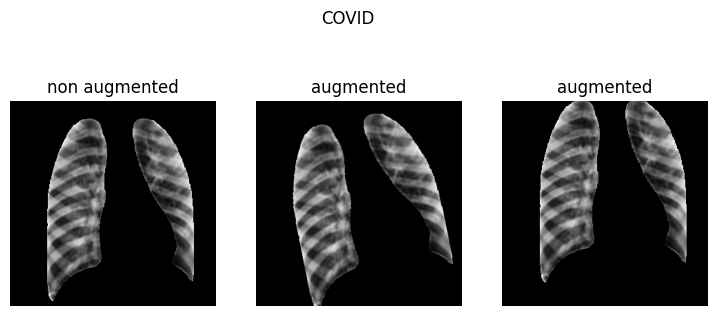
\includegraphics[width=1.0\linewidth]{aug_example_covid.png}
    \caption{Example of processed X-ray image combined with mask and its augmentations for the class "COVID".}
    \label{fig:aug_example_covid}
\end{figure}

\begin{figure}[H] % the [h!] helps force it "here"
    \centering
    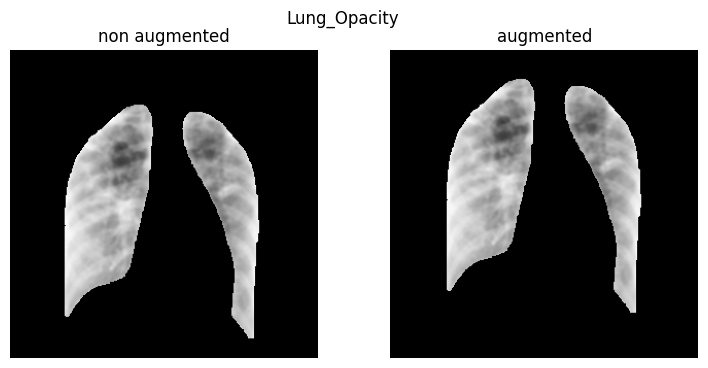
\includegraphics[width=0.65\linewidth]{aug_example_lung_opcacity.png}
    \caption{Example of processed X-ray image combined with mask and its augmentations for the class "Lung opacity".}
    \label{fig:aug_example_lung_opcacity}
\end{figure}

\begin{figure}[!htb] % the [h!] helps force it "here"
    \centering
    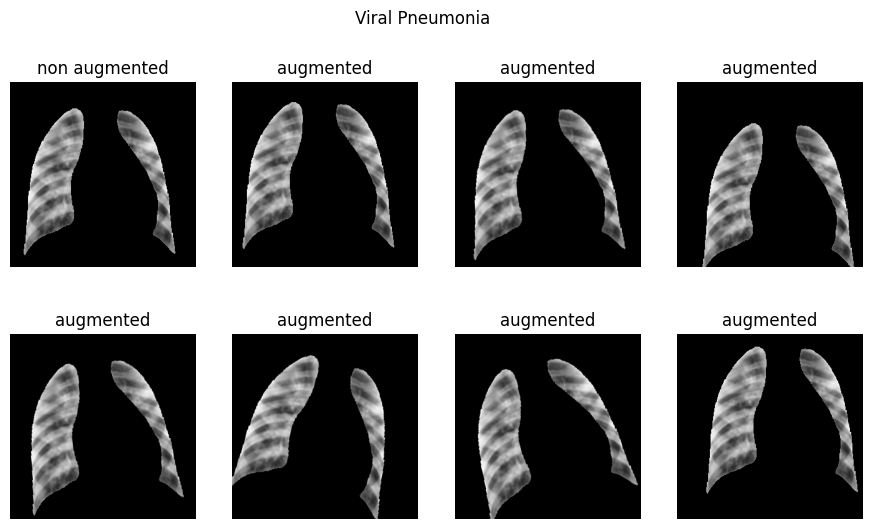
\includegraphics[width=1.0\linewidth]{aug_example_viral_pn.png}
    \caption{Example of processed X-ray image combined with mask and its augmentationsfor the class "Viral pneumonia".}
    \label{fig:aug_example_viral_pn}
\end{figure}


\subsubsection{Feature Extraction}
Since we have a large dataset consisting of a total of 35059 images just in the train set it is a good idea to identify important features to reduce the computing time.
Extracting features reduces the image's size dramatically and converts it into a compact representation that's suitable for machine learning models. 

Chest X-ray images reveal structural differences in the lungs based on the condition. For example:
\begin{itemize}
    \item COVID-19 often shows bilateral ground-glass opacities.
    \item Viral / Bacterial Pneumonia can show localized consolidation or patchy opacities.
    \item Lung Opacity is a broader label that includes a range of conditions affecting lung transparency.
    \item Normal lungs have well-defined, clear lung fields.
\end{itemize}

\vspace{0.5cm}

To classify these visually distinct conditions, we need a way to extract structural patterns from grayscale X-ray images.\\

\noindent \underline{HOG:}
\vspace{0.5cm}\\
HOG, or Histogram of Oriented Gradients, is a feature descriptor used in computer vision and image processing.  
HOG captures the structure and edge directions in an image, which are crucial for identifying shapes and patterns.
\\

HOG Captures from X-rays

\begin{itemize}
     \item Edges of lung boundaries, rib cage, and lesions.
     \item Orientation and distribution of densities — darker/lighter areas correspond to tissue and opacity differences.
     \item Shape and spread of abnormalities, like how diffuse or sharp an opacity is.
\end{itemize}
Although HOG is handcrafted, not learned  and  so it may miss subtle texture or high-level patterns, it is a fast, interpretable, and memory-efficient way to 
extract features from chest X-rays. \\
We have a HOG (Histogram of Oriented Gradients) feature dataset with a shape of (35059, 8100), which means:
\begin{itemize}
    \item 35059 represents the number of images in your dataset.
    \item 8100 represents the number of features extracted from each image using the HOG method.
\end{itemize}
	
These 8100 features are typically a flattened representation of the gradients and orientations from the original image. Our image was originally a 299x299 
pixel image, the HOG algorithm works by breaking the image into smaller cells (e.g., 8x8 pixels per cell), compute the gradient orientations, 
and then describe the image based on these features. The 8100 features might correspond to a smaller, downscaled version of the original image, where each image
is transformed into a set of descriptive gradient-based features, rather than keeping the full raw pixel values.
In simpler terms, we are working with feature vectors derived from each image, not the full size of the image. Each of the 8100 features corresponds to a 
particular characteristic (such as the gradient of pixel intensity) of the image after applying the HOG technique.
So, (35059, 8100) indicates that we have 35059 images, and each image has been transformed into a feature vector of length 8100 after HOG processing.

\begin{figure}%[h!] % the [h!] helps force it "here"
    \centering
    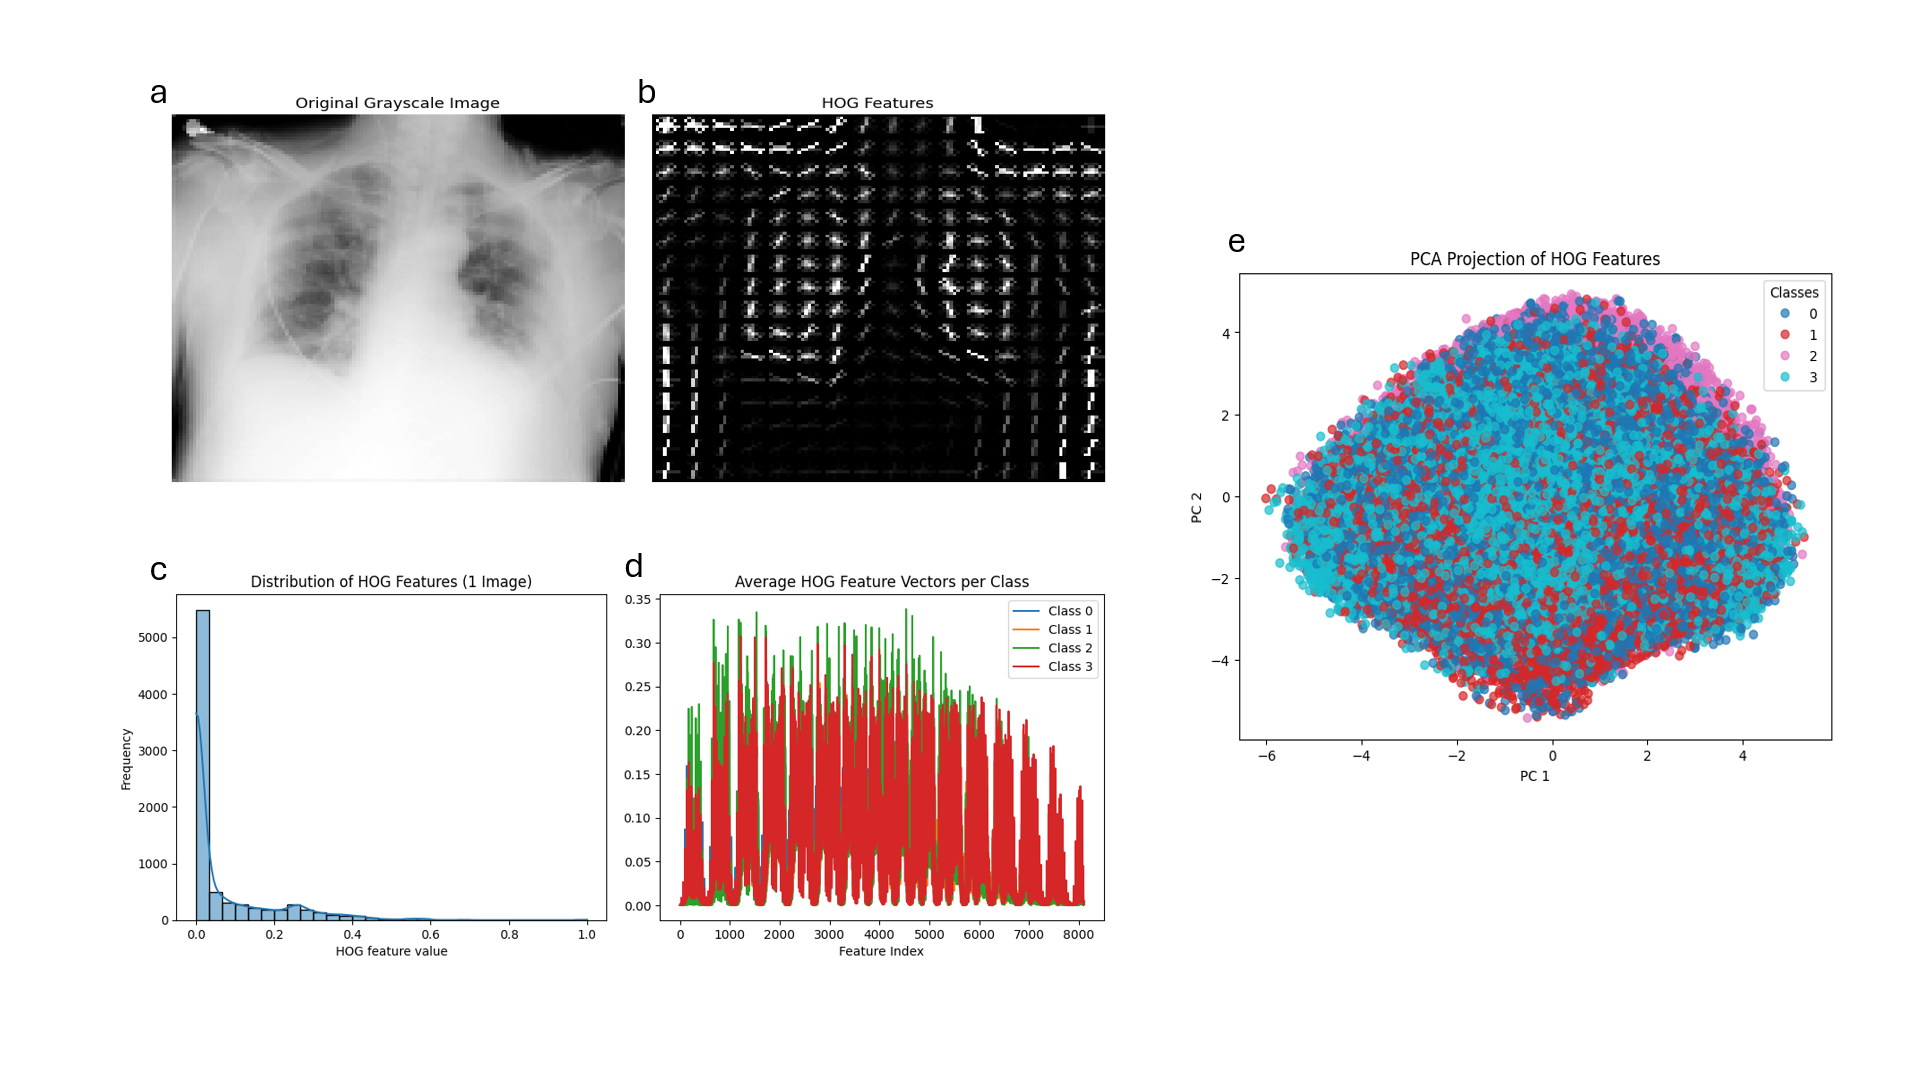
\includegraphics[width=1.0\linewidth]{hogfeatures_all.png}
    \caption{Visualisation of hog features}
    \label{fig:Visualisation of hog features}
\end{figure}
Figure \ref{fig:Visualisation of hog features}a shows the original grayscale image. We can clearly see the chest X-ray with anatomical structures like ribs and lungs.\\
Figure \ref{fig:Visualisation of hog features}b effectively displays edges and gradients, especially around the rib cage, clavicle, and lung boundaries. 
The blocky structure is normal due to the cell/block division of the HOG algorithm (e.g., 8x8 pixels per cell). The highlighted edges capture shape and 
orientation information, which HOG is designed to emphasize. The features look rich and well-distributed and are therefore useful for capturing structural patterns:\\
Figure \ref{fig:Visualisation of hog features}c displays the distribution of HOG Features per image. Most feature values are near zero (common in HOG due 
to sparse gradients) in the histogram and a long tail which represents stronger edges or corners.\\
The line plot shows the average HOG values across feature indices for each class used for class separability analysis 
(Figure \ref{fig:Visualisation of hog features}d). It helps identify which feature indices (spatial areas or orientations) contribute more for specific classes. 
Overlapping curves indicate similar structures between some classes (e.g., viral vs lung opacity).\\
We also plot a PCA projection of HOG characteristics (figure \ref{fig:Visualisation of hog features}e). The 2D scatter plot of HOG characteristics 
after reduction of dimensionality using PCA (Principal Component Analysis) showed significant overlap suggesting that HOG alone may not strongly separate 
some classes (hence the need for a classifier).
In summary, HOG works well visually, but it’s not sufficient alone for strong class separation in our dataset. Therefore for most our ML models, 
we use HOG features, but we also extracted deeper features using other methods like ResNet, VGG16 and GLCM.
\\

\vspace{0.5cm}
    

\subsection{ Flatten Features for ML Models}\label{flatten_features}
Input: Extracted HOG features (1D numpy array) for each image.\\
Operation: Flatten the 2D image representation into a single 1D array of features.\\
Output: A 1D numpy array for each image that can be used as input to machine learning models. This would typically be an array of shape (n\_samples, n\_features).\\
\subsection{Training Machine Learning Models}\label{train_ML}
Input: Feature arrays (flattened HOG features) and encoded labels.
Operation: Use machine learning models (e.g. Forest, Logistic Regression, XGBoost) to train on the feature vectors.
Output: A trained model that can predict the class (label) of new, unseen images based on their feature vectors.

\subsection{Metrics to Evaluate the Model Results} \label{metrics_ML}
Input: Trained machine learning model and the test set (augmented images, labels).\\
Operation: Evaluate the model's performance using metrics like accuracy, F1 score, and confusion matrix to understand how well it classifies the different 
image classes.\\
Output: Evaluation metrics to show true vs predicted labels.

There are also a number of hyperpramater tuning strategies, which we used in different modelling tests:
\begin{itemize}
    \item GridSearchCV
    \item RandomizedSearchCV
    \item BayesSearchCV
\end{itemize}

\subsection{Modelling and Results}
\begin{figure}%[ht] % the [h!] helps force it "here"
    \centering
    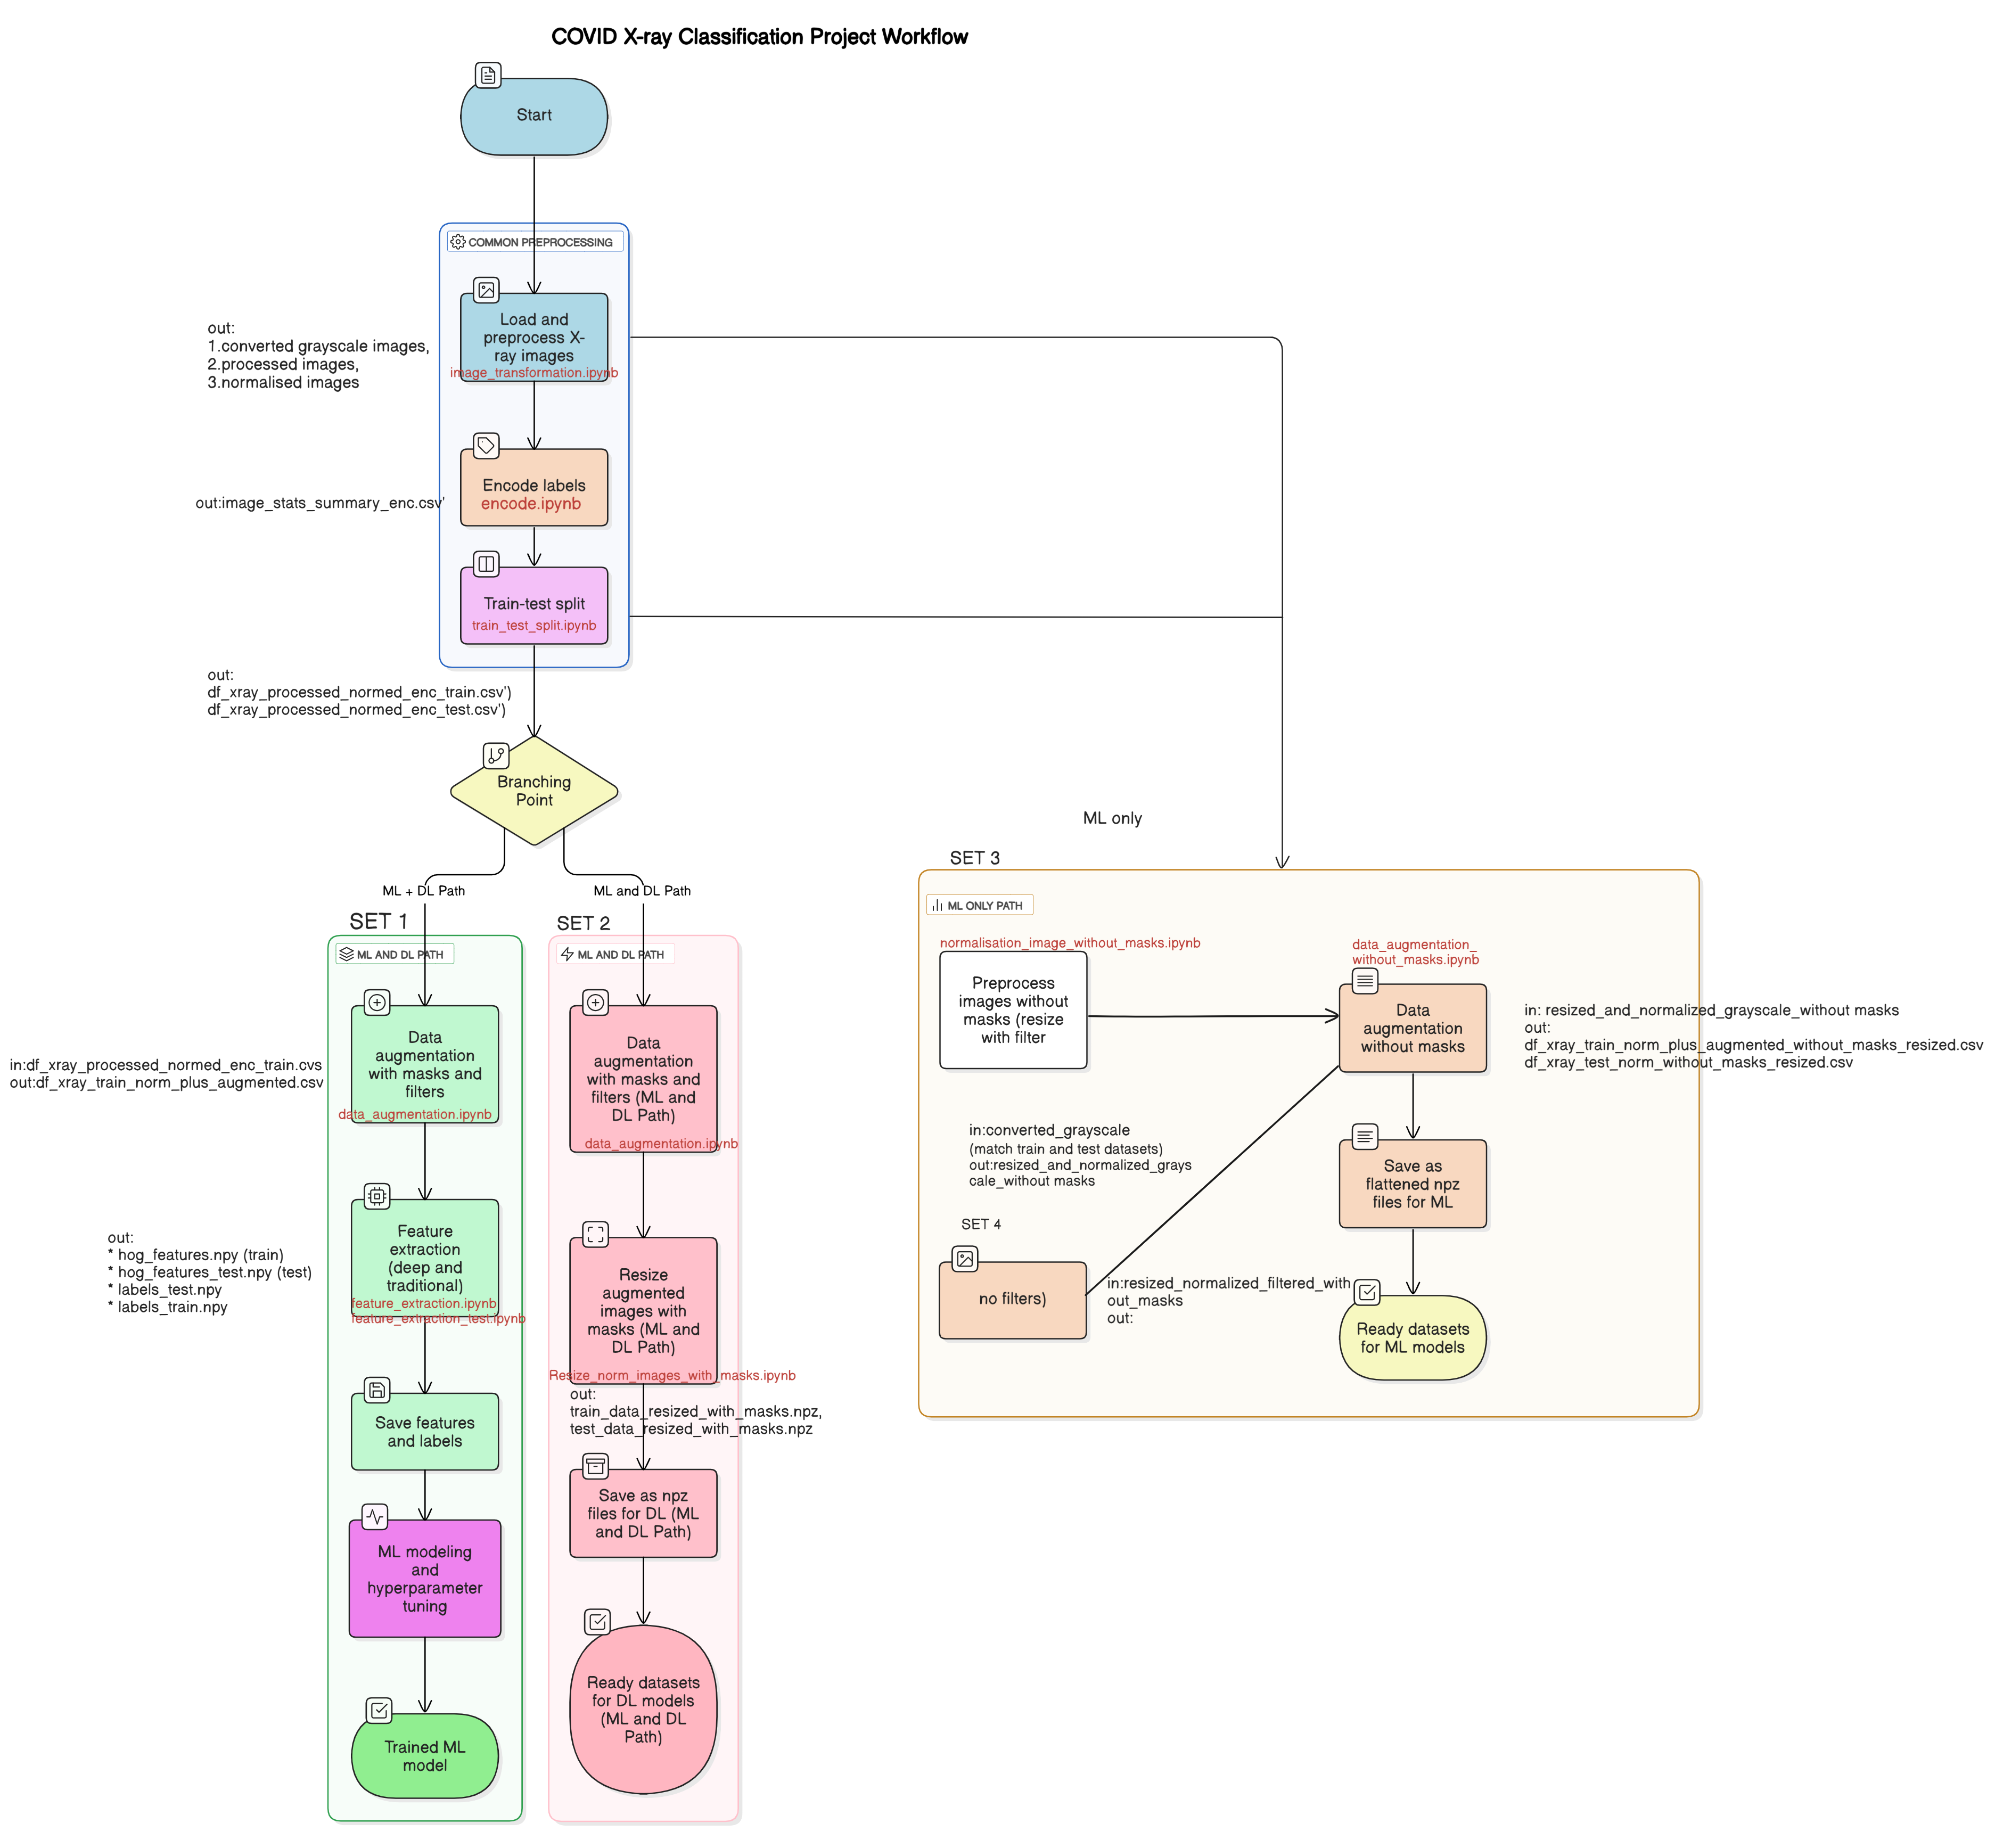
\includegraphics[width=1.0\linewidth]{diagram-export-5-8-2025-4_05_06-PM.png}
    \caption{Sets of images used for ML models}
    \label{fig:WORKFLOW}
\end{figure}
The \textbf{COVID X-ray Classification Project Workflow} outlines the complete pipeline for preparing and modeling chest X-ray data to classify COVID-19 and other conditions using machine learning (ML) techniques.

The process begins with loading and preprocessing the raw X-ray images, where they are converted to grayscale, resized, and normalized using the \texttt{gray\_image.ipynb} script.

Next, labels are encoded into a machine-readable format using \texttt{encode\_labels.ipynb}, and the dataset is split into training and testing sets with \texttt{train\_test\_split.ipynb}.

At this stage, the workflow branches into three sets.

\textbf{SET 1} involves using feature extraction methods such as Histogram of Oriented Gradients (HOG). The extracted features and labels are saved for model training and hyperparameter tuning.

\textbf{SET 2} applies masks and filters during data augmentation. These images are resized to 128*128 and 20*20 pixels. The augmented images and labels are saved as \texttt{.npz} files for use in ML pipelines.

\textbf{SET 3 } preprocesses images without applying filters by resizing and normalizing them, followed by augmentation without masks. The resulting data is then flattened and stored as \texttt{.npz} files for traditional ML models.

\textbf{SET 4 }preprocesses images after applying filters by resizing and normalizing them.

With this workflow we wanted to ensure a structured and modular approach to data handling, augmentation, feature extraction, and model training.
\\

\subsubsection{Logistic Regression}
We started with logistic regression as it serves as a baseline for performance. Also, it is computationally inexpensive and we can quickly iterate over different versions, features and preprocessing methods. In logistic regression, C is the regularization strength while the solver defines the optimization algorithm.	Regularization helps prevent overfitting (when our model memorizes training data instead of learning patterns).
C is inversely related to regularization:
\begin{itemize}
    \item A smaller C means stronger regularization (simpler model).
    \item A larger C means weaker regularization (more flexible model).
\end{itemize}
Also, we need to test different solvers to see which performs best:
\begin{itemize}
    \item liblinear for binary, small-to-medium-sized data.
    \item lbfgs or saga for larger datasets or multi-class problems.
\end{itemize}

\textbf{1st trial}: Hog features (Figure \ref{fig:Logistic_Regression}A). We gave the model HOG features, a fingerprint of edges. This helped the computer guess pretty well.
This model gave an accuracy of 73.71\% overall, the best performance, especially for COVID \& Pneumonia.
\\
\textbf{2nd trial}: Images with masks resized (Figure \ref{fig:Logistic_Regression}B). We shrunk the image small and used masks. It didn’t help much.
We got an Accuracy: 58.04\%. The model made bad guesses, especially for Normal and COVID images however Pneumonia class had high recall (0.90) but low precision (0.42).
\\
\textbf{3rd trial}: Images without masks resized without filters (Figure \ref{fig:Logistic_Regression}C) we also fed the model same small images, but now the whole image is visible. This increased the accuracy to 69.24\%  and displayed a nice balance across all disease types.
\\
\begin{figure}[H] % the [h!] helps force it "here"
    \centering
    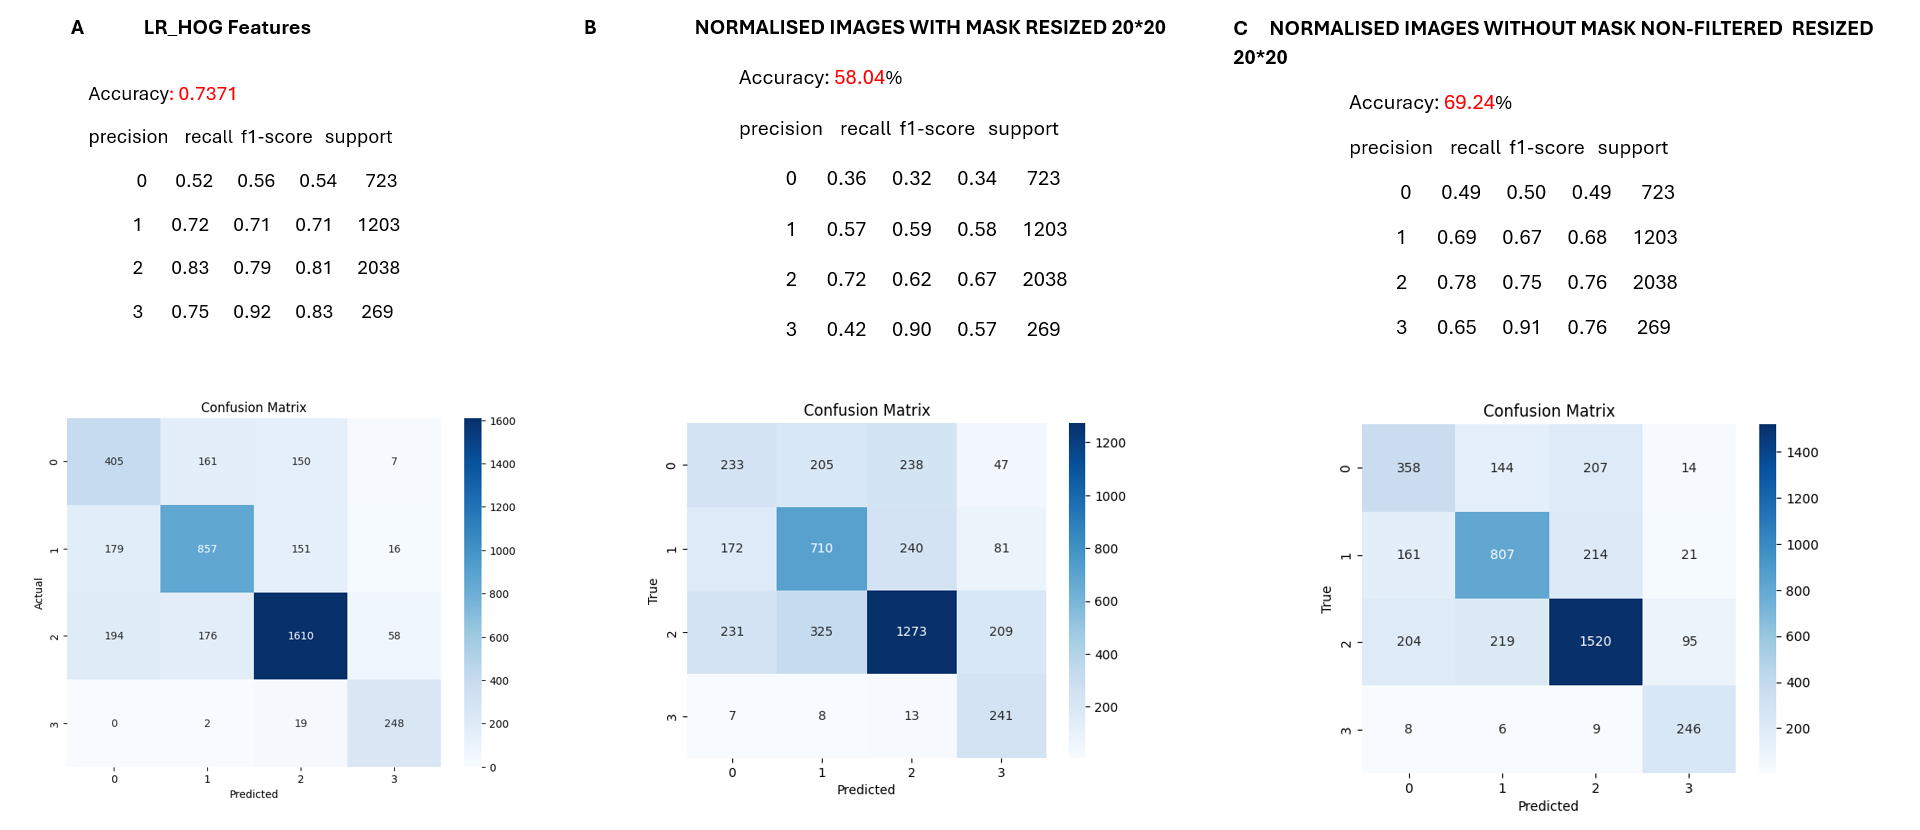
\includegraphics[width=1.0\linewidth]{lr1,2,3.png}
    \caption{Logistic Regression models A, B, C}
    \label{fig:Logistic_Regression}
\end{figure}
\textbf{4th trial}:Random grid search + PCA (Figure \ref{fig:Logistic_Regression_logreg2} A)
While running a GridSearch on HOG features, my system ran out of memory and crashed. To make the training more manageable, I switched to RandomizedSearchCV combined with PCA to reduce dimensionality.
Here we used SAG (Stochastic Average Gradient) which is ideal for large datasets and when we want faster convergence of SGD without noisy updates. It works by iterating through the data in mini-batches. In each iteration, it computes the gradient (slope of the cost function) for each mini-batch, and averages them to update the parameters. Over time, this leads to more stable and faster convergence compared to regular SGD (Stochastic Gradient Descent). Also, for dimensionality reduction PCA was used which reduced features to 100 components.
Using a random grid with PCA we improved the accuracy to 65.37\%, which is solid for logistic regression with HOG characteristics. The best parameters found were C = 0.075, penalty = L1. The PCA retained variance 62\% and showed a better precision-recall balance in COVID class.\\
Class-wise performance: 
\begin{itemize}
    \item Class 2 (2038 samples): Highest F1 (0.74), meaning our model is best at detecting this.
    \item Class 3 (269 samples): Very high recall (0.93) but low precision — it’s over-predicting this class.
    \item Class 0 and 1: More balanced, but weaker F1.
The accuracy drop may be because of the pca which we set to 100.
\end{itemize}

\textbf{5th trials}: Gridsearch cv (Figure \ref{fig:Logistic_Regression_logreg2}B)
We applied Grid Search on normalized, unmasked, non-filtered 20×20 images to obtain the best Params: C=0.1, penalty=L2 and an accuracy of 69.10\%.
Logistic regression after hyperparameter tuning showed slight improvement in accuracy and confusion matrix and displayed a	similar class-wise performance to the base version. The raw HOG features might have contained valuable info that PCA compressed away in the previous model.
\\
\textbf{6th trial}:Manual Parameter Tuning using CuML on HOG features (Figure \ref{fig:Logistic_Regression_logreg2}C).
We then revisited GridSearch with cuML on hog features, which is faster because it uses the GPU.
Here we set solver='qn' in cuML's Logistic Regression (i.e., GPU-accelerated version), and it refers to the Quasi-Newton method.
Quasi-Newton is a family of optimization algorithms used to minimize a function (like the logistic loss).
It is similar in spirit to lbfgs in scikit-learn (also a Quasi-Newton method). It does not support L1 regularization — only L2.
In this experiment, we trained a CuML Logistic Regression model using a subset of the training data (5000 samples) with GPU acceleration to enhance performance. The model utilized \texttt{class\_weight='balanced'} to address class imbalances. This model was fast and efficient and gave the same result as best one (HOG) with an accuracy: 73.47\% on the test set.

The classification report reveals that the model's recall is highest for the Normal (2) class (85\%)and Viral Pneumonia (3) (82\%), while the lowest recall is for COVID (0) (39\%). The precision and F1-scores also reflect this imbalance, with the model performing better on the more frequent classes.
\\
Summary:
\begin{itemize}
    \item HOG features yielded the best accuracy (~73.7\%) with strong recall on Pneumonia and COVID.
    \item Raw pixel features (even when resized) underperformed compared to HOG or PCA-based features.
    \item PCA compressed HOG features to retain 62\% variance, resulting in slightly reduced performance but possibly lower model complexity.
    \item Logistic regression benefited modestly from hyperparameter tuning (Grid and Random Search), but improvements were incremental.
    \item Pneumonia class consistently showed high recall but variable precision.
\end{itemize}
In conclusion, the Logistic Regression Model on hog features with Best C: 0.01 obtained by performing manual tuning using Cuml gave us the best accuracy (73\%)
Room for Improvement: Logistic regression might not be the best choice for such a high-dimensional feature set. Therefore, we next chose to experiment with other models like Support Vector Machines (SVM) and Random Forests, which could perform better without requiring dimensionality reduction.


\begin{figure}[H]
    \centering
    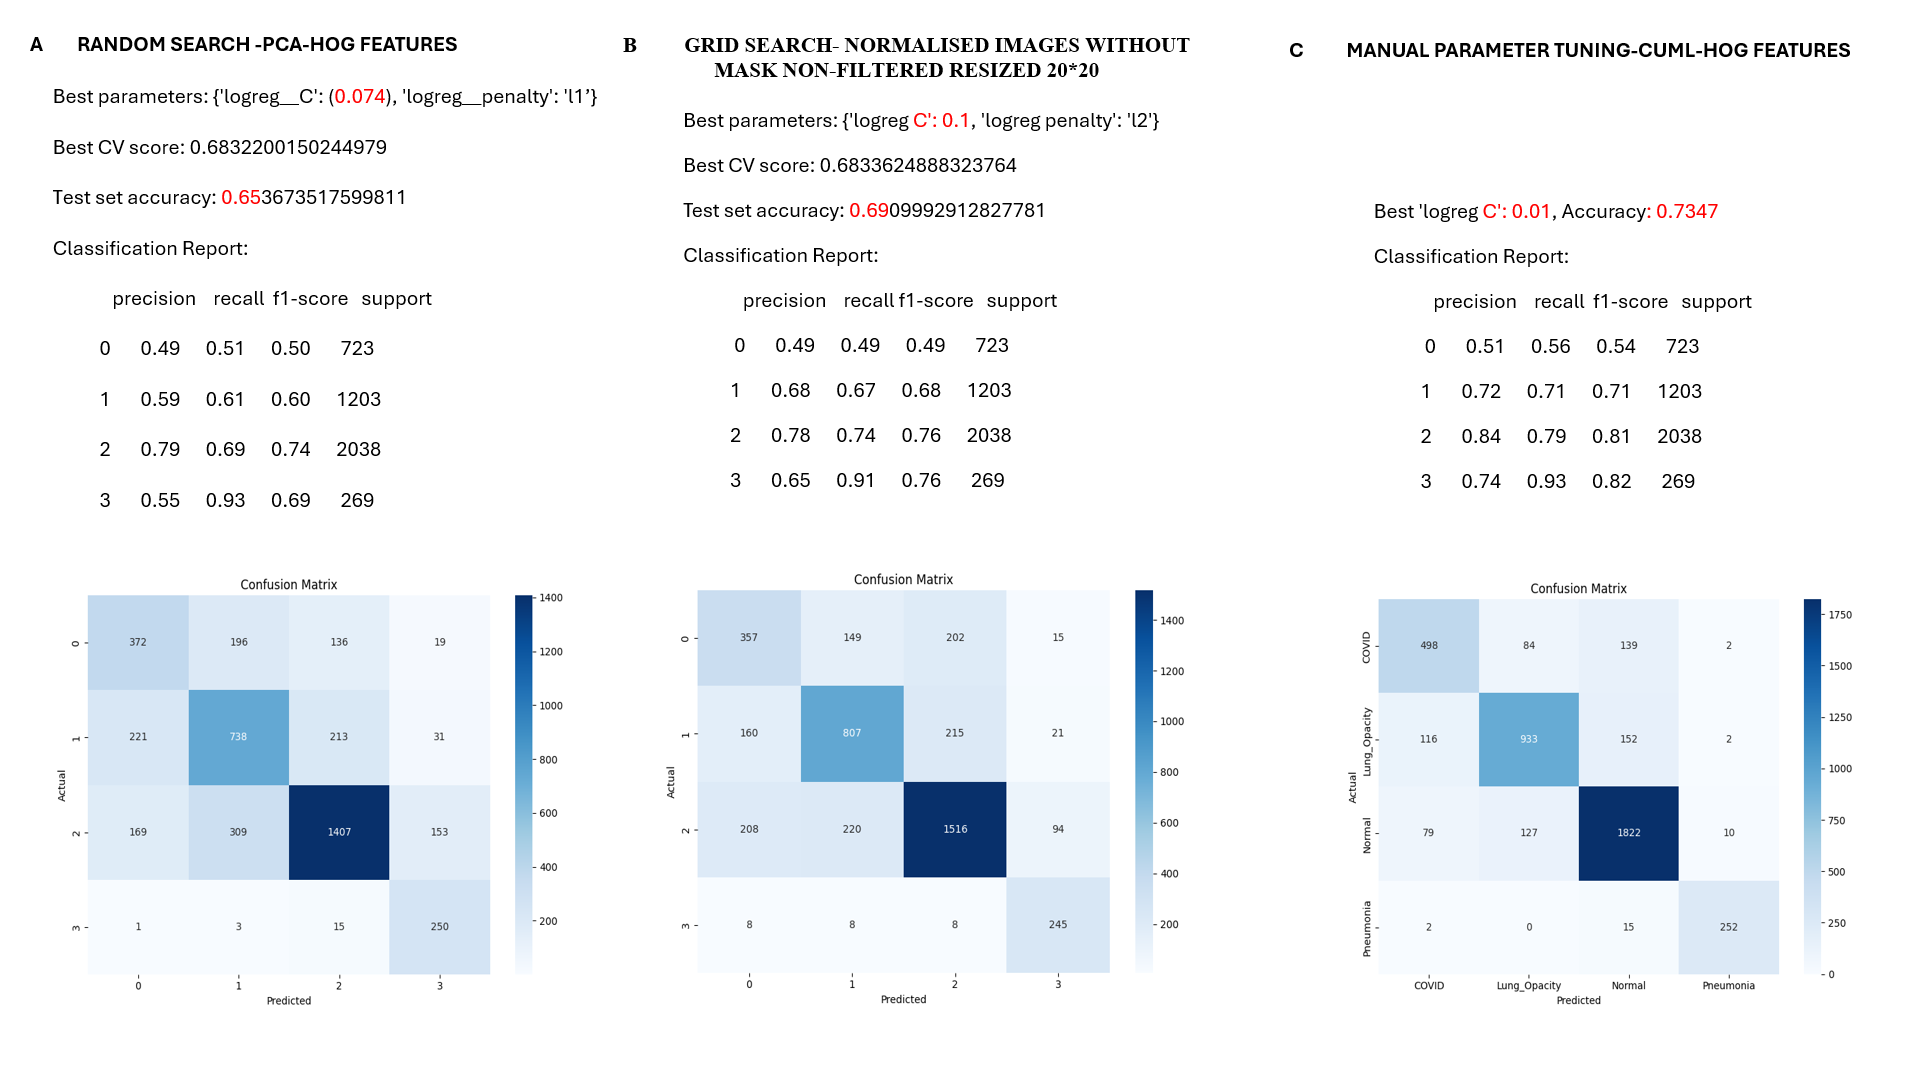
\includegraphics[width=1.0\linewidth]{logreg2,a,b,c.png}
    \caption{More Logistic Regression models A, B, C}
    \label{fig:Logistic_Regression_logreg2}
\end{figure}


\subsubsection{Random Forest}
The Random Forest model is an ensemble learning method that combines multiple decision trees to improve classification accuracy and robustness. It works by creating a multitude of decision trees during training and outputting the mode of their predictions (for classification tasks). 
The main advantages of Random Forest include:
\begin{itemize}
    \item It handles high datasets with high-dimensional data well, making it suitable for image classification tasks.
    \item Robustness to noise and overfitting, as it averages the predictions of multiple trees.
    \item Paralellization, which allows for efficient use of computational resources.
    \item Improved accuracy and reduced variance compared to individual decision trees.
\end{itemize}
The disadvantages of the model include:
\begin{itemize}
    \item It can be slower to train than simpler models like logistic regression, especially with large datasets.
    \item It may not perform as well on very small datasets or when the number of features is much larger than the number of samples.
    \item Training and prediction can be computationally expensive, especially with many trees or large datasets.
    \item Imbalanced datasets may pose a challenge, as the model may favor the majority class.
\end{itemize}
\textbf{1st trial}: Random Forest with default hyperparameters:\\
The first attempt at using the Random Forest model for our classification problem does not specify any hyperparameters. It uses the HOG features as inputs. The score obtained by this model is 0.7602173399480274

\begin{figure}[H]
    \centering
    \begin{minipage}[t]{0.48\textwidth}
        \centering
        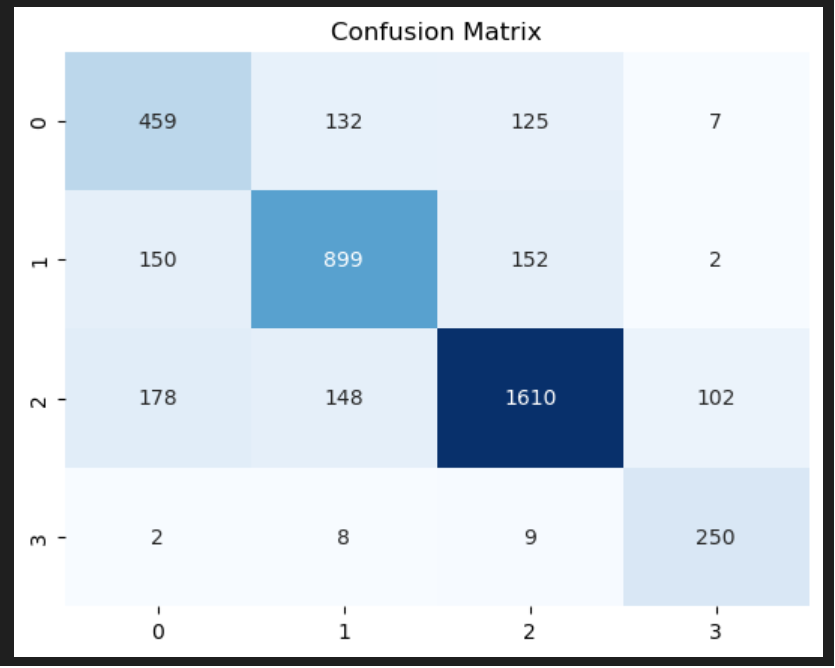
\includegraphics[width=\linewidth]{CM_RF_default.png}
        \caption{Confusion Matrix}
        \label{fig:confusion_rf_default}
    \end{minipage}
    \hfill
    \begin{minipage}[t]{0.48\textwidth}
        \centering
        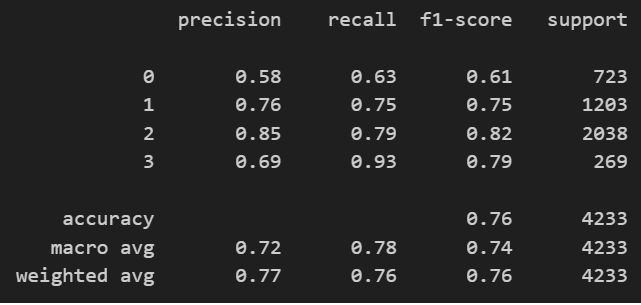
\includegraphics[width=\linewidth]{CR_RF_default.png}
        \caption{Classification Report}
        \label{fig:classification_rf_default}
    \end{minipage}
\end{figure}
In the pictures above, the encoded labels are:
\begin{itemize}
    \item COVID: 0
    \item Lung Opacity: 1
    \item Normal: 2
    \item Viral Pneumonia: 3
\end{itemize}
The result is better than the Logistic Regression Model. However, the f1 score for the COVID category is the lowest. We tried to improve this score by finding a proper set of hyperparameters. 

\textbf{2nd trial}: Parameter optimization for Random Forest with GridsearchCV:\\
We tried to optimize parameters using the HOG features as inputs, but the memory requirements and computing time were prohibitive. We chose to use the normalized, unmasked, non-filtered 20×20 images. 
Best parameters found are:
\begin{itemize}
    \item class weight: balanced
    \item max depth: 50
    \item max features: log2
    \item min samples leaf: 1
    \item number of estimators: 300
\end{itemize} 
Best cross-validation score was  0.8406127980473902.

\begin{figure}[H]
    \centering
    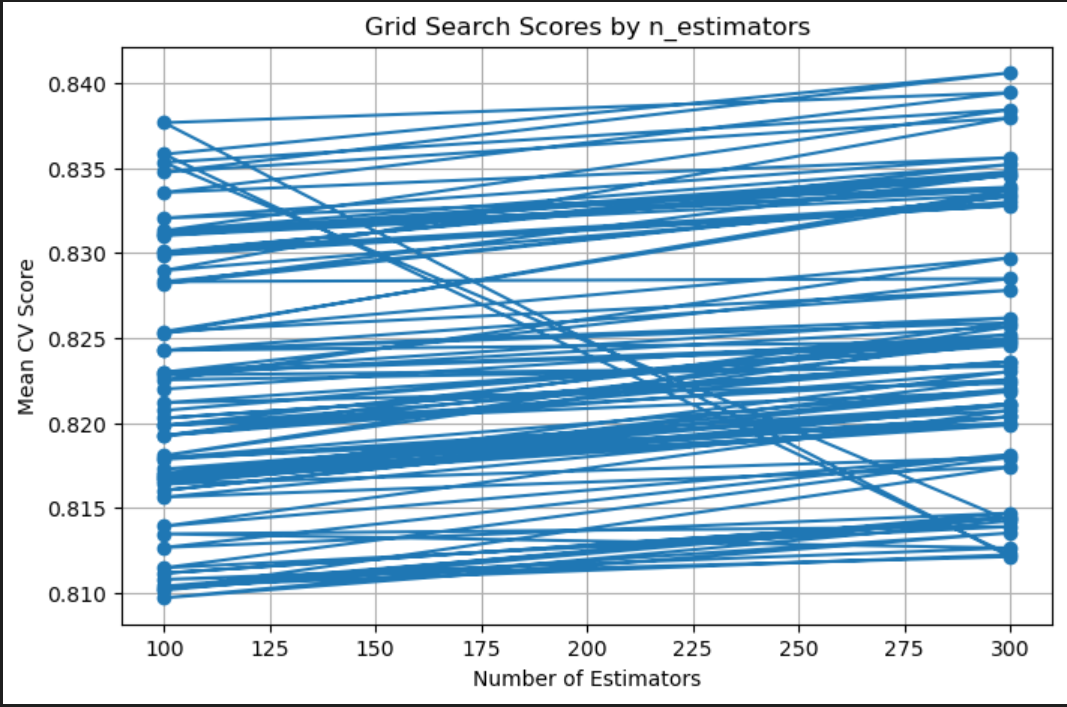
\includegraphics[width=0.8\linewidth]{GridSearchScore.png}
    \caption{Grid Search Score}
    \label{fig:GridSearchCV}
\end{figure}

\textbf{3rd trial}: Random Forest with optimal hyperparameters previously determined:\\
Using the balanced class weight, the max depth 50, log2, 300 estimators and 1 min samples leaf, we generated a Random Forest Classifier and trained it with the HOG features. The results are shown below: 

\begin{figure}[H]
    \centering
    \begin{minipage}[t]{0.48\textwidth}
        \centering
        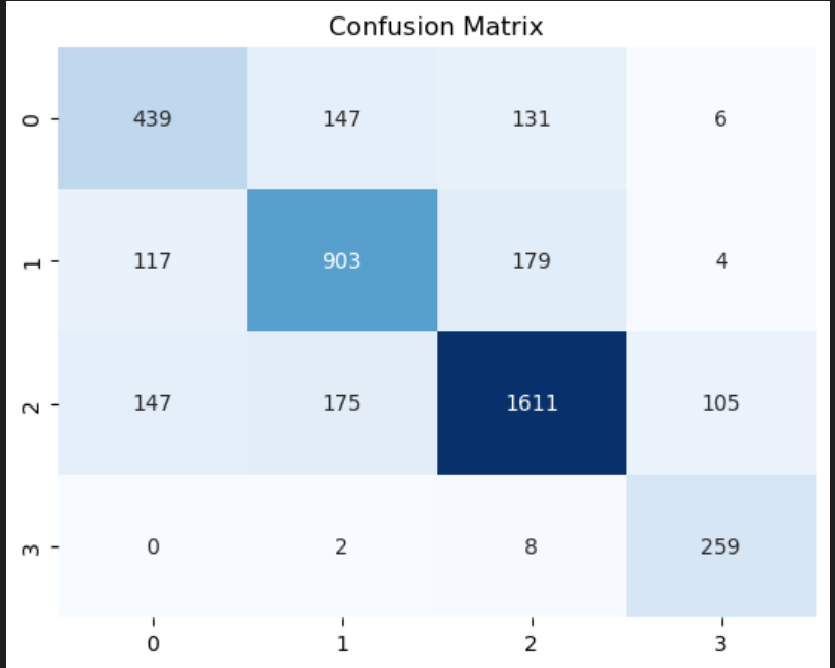
\includegraphics[width=\linewidth]{CM_RF_opt.png}
        \caption{Confusion Matrix}
        \label{fig:confusion_rf_opt}
    \end{minipage}
    \hfill
    \begin{minipage}[t]{0.48\textwidth}
        \centering
        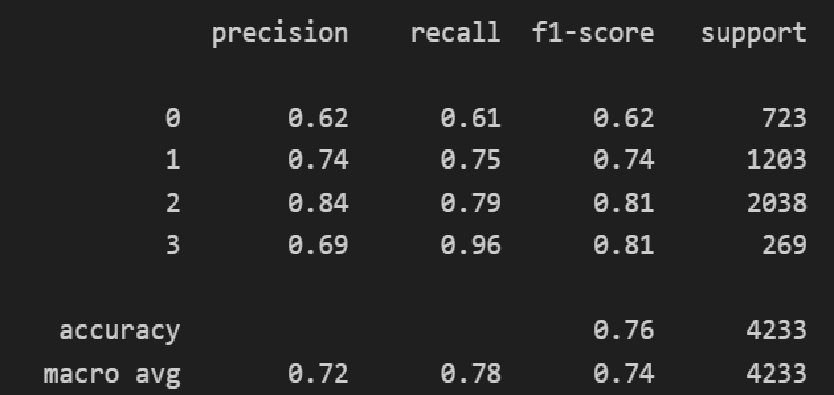
\includegraphics[width=\linewidth]{CR_RF_opt.png}
        \caption{Classification Report}
        \label{fig:classification_rf_opt}
    \end{minipage}
\end{figure}

The overall score is not better than the one obtained with default parameters. However, there is a small improvement in the f1 score for the COVID category.
In conclusion, the Random Forest is not the optimal model to analyze COVID X-rays. 

\subsubsection{Support Vector Machines (SVM)}
There are two types of SVM models: linear and nonlinear SVM. Here's a brief summary of both: \\
\underline{Linear SVM:}
\begin{itemize}
    \item Separates data using a straight line (in 2D) or a hyperplane (in higher dimensions).
    \item Assumes that the data is linearly separable (i.e., classes can be separated by a straight boundary).
    \item Uses a linear kernel.
    \item Fast and efficient for high-dimensional, sparse data like text or HOG features.
    \item Good for: When the data has clear linear boundaries.
\end{itemize}
\underline{Nonlinear SVM:}
\begin{itemize}
    \item Can separate data with curved or complex boundaries.
    \item Uses kernel tricks (e.g., RBF, polynomial) to map the data into higher dimensions where it may become linearly separable.
    \item More flexible but computationally expensive, especially on large datasets.
    \item Good for: Data where classes are intertwined and not separable by a straight line.
\end{itemize}

In the following tests we used nonlinear and linear SVMs. As our task  is a classification problem we used SVC models.

\textbf{1st trial}\\
The first trial to run a SVG model was with a dataset with preprocessed images and added masks. The image size was reduced to 128x128 pixels, and we tried 
to use the entire training dataset (approx. 35'000 images). For this first attempt no hyperparameter optimization technique was used. Instead, we tried some random 
hyperparameters: 
\begin{itemize}
    \item gamma=0.01
    \item kernel='poly'
    \item other hyperparameter were left to default
\end{itemize}
After over 6 hours the training of the model was not finished. We stopped it, because this approach had proven as impractical. As it took that much time even without
using a hyperparameter optimization technique like GridSearchCV, we needed to change the dataset (number or/ and size of images) for further tests.


\textbf{2nd trial}\\
For the second trial we tried to work with a considerably smaller dataset to reduce the training speed. The aim was to get a SVC model running. And maybe in future 
tests reenlarge the dataset again. Therefore, we reduced the size of the images and aswell the number (20x20 pixels and only 2000 images randomly chosen from the train 
dataset). In this run we tried to use GridSearchCV to find the best parameters out of these options: 
\begin{itemize}
    \item C: 0.1, 1, 10, 100
    \item loss: 'hinge', 'squared\_hinge'
    \item max\_iter: 100, 1000
\end{itemize}

The best hyperparameter set was: C = 10,  gamma = 0.001 and kernel = rbf. The runtime was approx. 12 minutes. The classification report in figure 
\ref{fig:SVC_2000_20x20_grid}a shows that the model has an overall accuracy of 65\%, but the prediction of class 0 (COVID) is very poor with a f1-score of only 0.29. The "normal" class could be best 
predicted which can also be seen on the confusion matrix in figure \ref{fig:SVC_2000_20x20_grid}b.

\begin{figure}[!ht]
  \centering
  \subfloat[][]{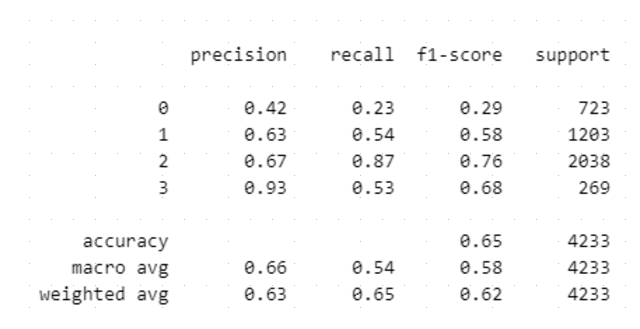
\includegraphics[width=0.4\linewidth]{SVC_grid_20_mask_slice2000_cf_report.png}}%
  \qquad
  \subfloat[][]{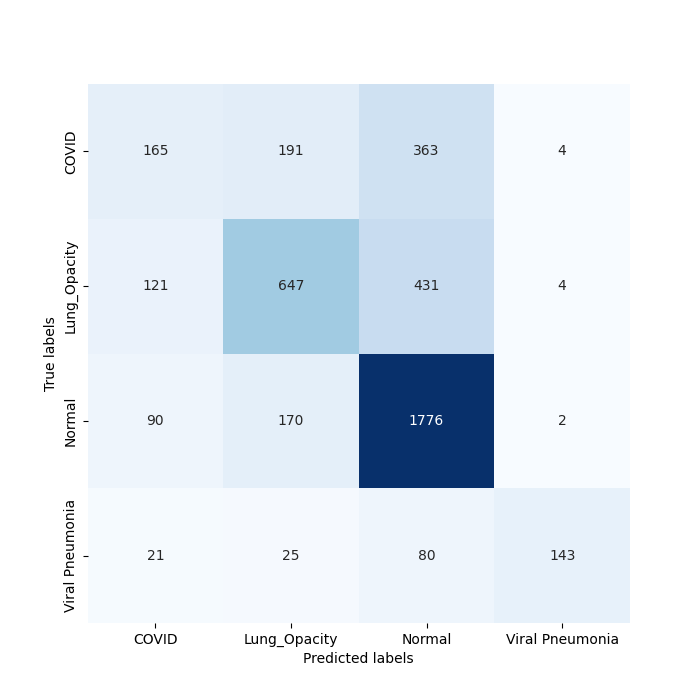
\includegraphics[width=0.4\linewidth]{SVC_grid_20_mask_slice2000_cm_abs.png}}%
  \caption{SVC model with 2000 images of size 20x20 pixels, best model with GridSearchCV (C = 10,  gamma = 0.001 and kernel = rbf)}
  \label{fig:SVC_2000_20x20_grid}
\end{figure}



\textbf{3rd trial}\\
Before trying to take more images with higher resulution, we tried to find options to make the training of the model faster.\\
One idea was to use another method for the hyperpramater optimization. We tested "Bayesian Optimization" instead of GridSearchCV as it does not test every 
combination of parameters, we hope that Bayes Optimization could be a faster option.\\
The input data for this test was the same as in the previous test. The "Bayesian Optimization" found the same hyperparameters as in the previous test but finished 
within only approx. 4 minutes. As this hyperpramater optimization method is about 3 times faster than GridSearchCV we will use this method for the next test with SVC 
when we'll try to use more images with more pixels. \\
Before doing further tests with the SVC model we did some research and found out, that SVC is not the best option for modelling with a lot of data. 
If using more images and images with more pixels, we increase the number of rows AND the number of columns in our data frame. This means we have a lot more input
data for our SVC model. The result of the search on the internet was, that using a linear SVC model could be a better option in our case. 

\textbf{4th trial}\\
As a conclusion of the previous tests we tried out a linear SVC model and used "Bayesian Optimization" for the hyperparameter search.\\
The number of pixel was increased to 128x128 pixels and the number of images was increased as well. We used 4000 non-augmented images (1000 of each class) to  which all
preprocessing steps from \ref{preprocessing_pipeline} apart from data augmentation and feature extraction have been apllied. \\

The best hyperparameter set was: C = 0.1,  loss = hinge, max\_iter=277. The runtime was approx. 1 hour. The classification report in figure 
\ref{fig:SVC_4000_128x128_bayes}a shows that the model has an overall accuracy of only  57\%, but the prediction of class 0 (COVID) is  with a f1-score of 
only 0.44. With a f1-score of 0.83 the "Viral pneumonia" class (3) is predicted better, which can also be seen on the confusion matrix in figure 
\ref{fig:SVC_4000_128x128_bayes}b.

The time needed to fit the model was about 1 hour, which is a lot for such poor prediction results. Maybe the model would perform better if more images or more pixels per image would be used. But due to the long training times we considered a training with more images not as an option.\\
Therefore, we decided to do further tests with a SVC linear model not with the images but with extracted features.\\

\begin{figure}[!ht]
  \centering
  \subfloat[][]{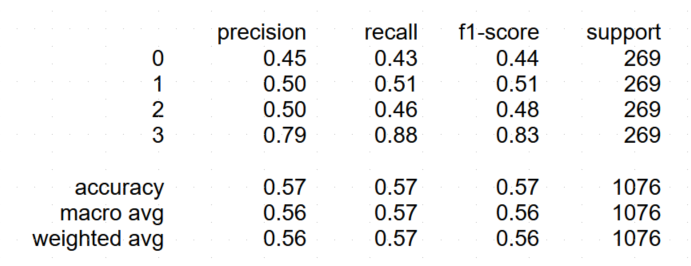
\includegraphics[width=0.4\linewidth]{SVClinear_bay_128_no_aug_mask_cf_report.png}}%
  \qquad
  \subfloat[][]{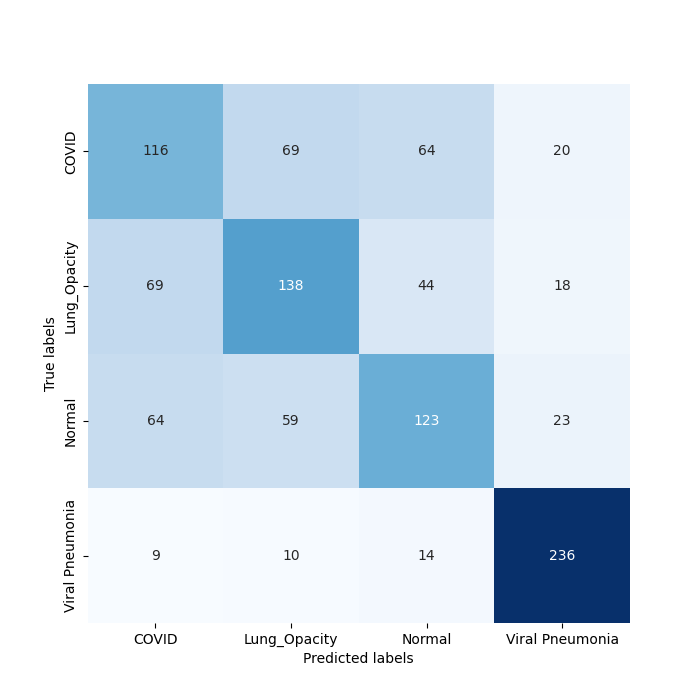
\includegraphics[width=0.4\linewidth]{SVClinear_bay_128_no_aug_mask_cm_abs.png}}%
  \caption{SVC model with 4000 images of size 128x128 pixels, best model with Bayes (C = 0.1,  loss = hinge, max\_iter=277)}
  \label{fig:SVC_4000_128x128_bayes}
\end{figure}


\textbf{5th trial }SGDClassifier (Linear SVM) + HOG (With hyperparameter search) Figure \ref{fig:SVM_MODELS}A. SGD still supports hinge loss, so it behaves like a linear SVM and also Supports L1, L2, ElasticNet regularization. In this model we used Randomized searchCV best estimator pipeline (Standandr Scaler, PCA, SGD classifier). \begin{verbatim}
Best Hyperparameters found were:
{'clf__penalty': 'l1', 'clf__learning_rate': 'optimal', 'clf__alpha': 0.001}
\end{verbatim}
We observed low overall accuracy (56.89\%), however the recall for the COVID class (class 0) was better at 63.07\%, and even stronger for Viral Pneumonia (class 3) at 86.62\%.\\
Perhaps Linear models like SGDClassifier may not fully capture complex patterns.
Therefore, the next steps would be to :
\begin{itemize}
    \item try a Tree-based Model e.g. XGBoost or LightGBM which handle non-linear relationships well and work directly on HOG features (no need to resize images)
    \item experiment with non-linear SVM on a subset of our data (e.g., 2–5k images) to test potential gains
\end{itemize}
\textbf{6th trial } So the next model we tested was grid search on nonlinear SVM using kernel rbf using a smaller dataset (5000) of hog features (Figure \ref{fig:SVM_MODELS}B). We performed grid search with reduced parameter space.  Accuracy improved to 72\%, and we found the Best parameters: \texttt{svc\_ C= 1},\texttt {svc\_ gamma = scale}.
\\
\begin{figure}[htb!] % the [h!] helps force it "here"
    \centering
    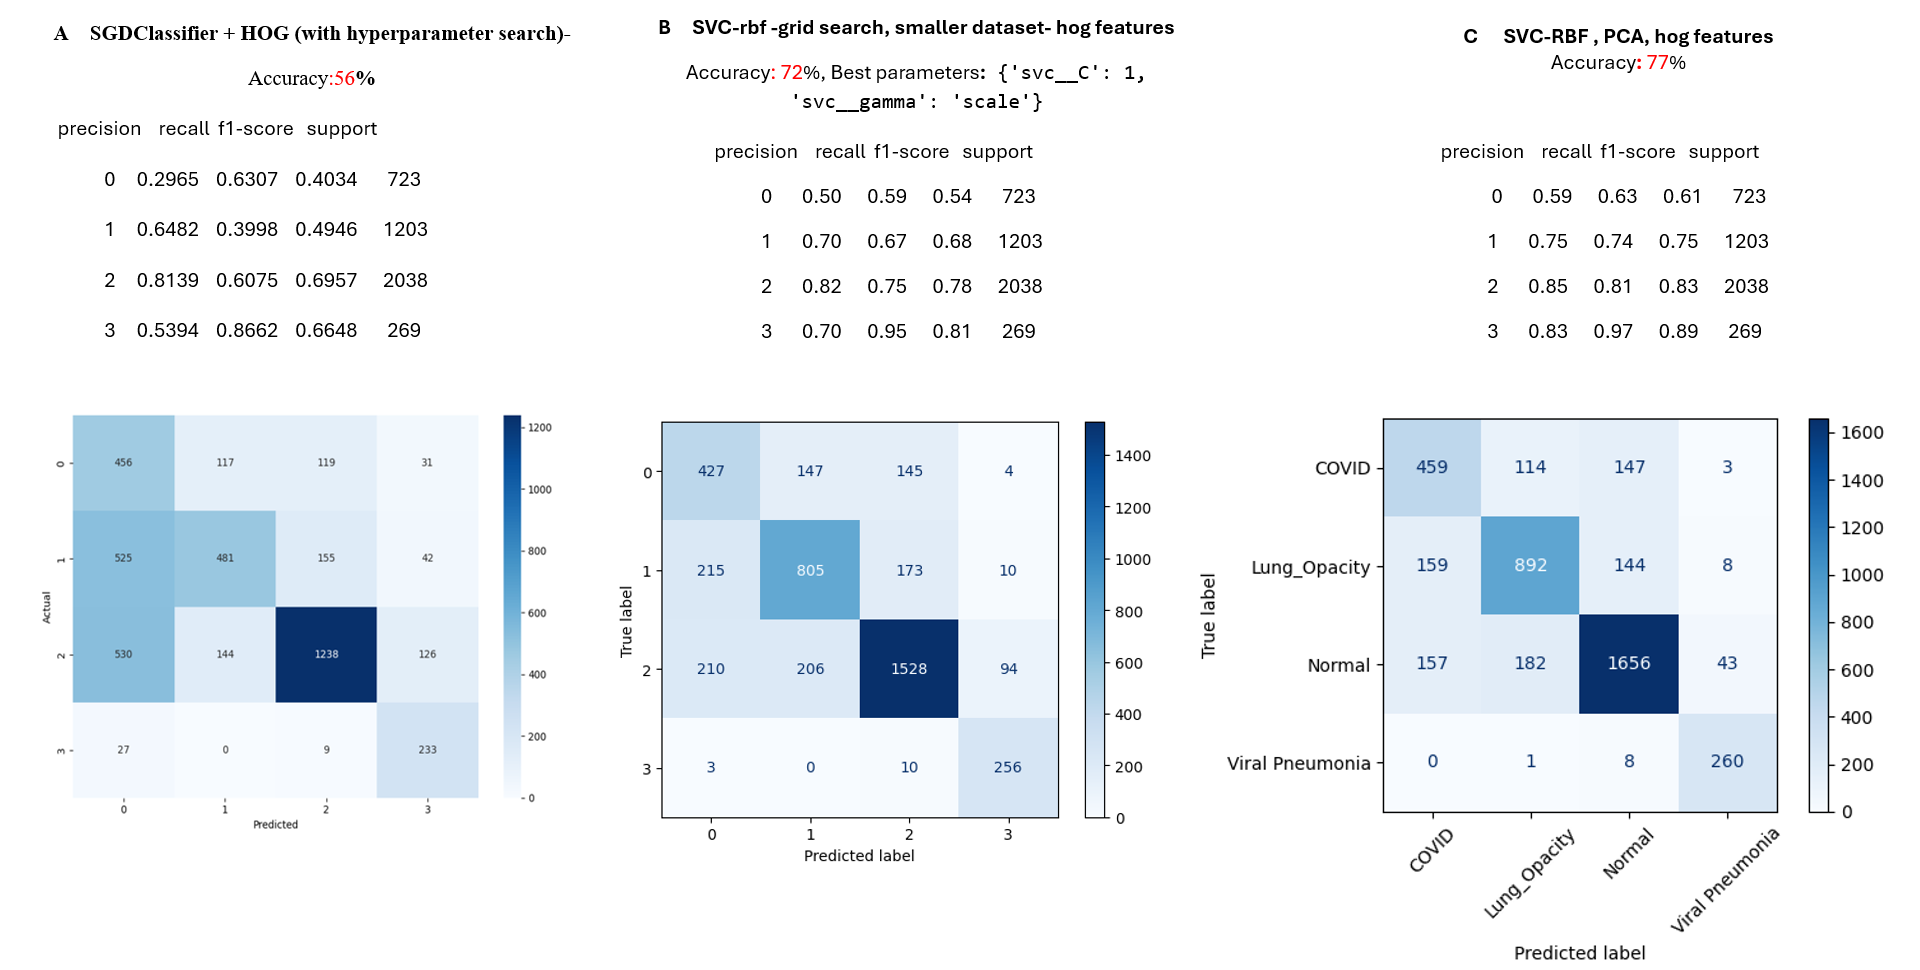
\includegraphics[width=1.0\linewidth]{svm ABC.png}
    \caption{SVM MODELS}
    \label{fig:SVM_MODELS}
\end{figure}
\textbf{7th trial }Since SVC\- RBF kernel gave us better results we decided to run it on hog features after dimensionality reduction using PCA. We observed an accuracy of 77\%. The Cumulative explained variance for PCA by 200 components was 62.06\%. However, the precision and recall for class 0 did not show much improvement and therefore, we proceeded with other ML models.\\


In conclusion, the SVC model with RBF kernel on Hog features with PCA dimensionality reduction gave us the best accuracy of 77\%.

\subsubsection{XGBoost - Extreme Gradient Boosting}
XGBoost (Extreme Gradient Boosting) can be used for classification and regression problems. It is a popular tool often used in machine learning 
competitions and  known  for handling large datasets efficiently. After the not very successful tests with e.g. SVM, the use of XGBoost looked promising.

Here is a summary of hyperparameters we used: 

\begin{itemize}
    \item booster = gbtree
    \item  objective = multi:softprob
    \item learning\_rate = 0.3
    \item tree\_method = hist
    \item num\_class = 4
    \item other hyperparameter were left to default
\end{itemize}

\textbf{1st trial} - XGBoost (128 x 128, non-augmented 4000 images, non augmented, with masks) \\
For the first test with the XGBoost model we used the same input data as in the 4th trial with the SVM model. The number of pixel was 128x128 pixels and the number 
of images was 4000 non-augmented images (1000 of each class). To these images all preprocessing steps from \ref{preprocessing_pipeline} apart from data 
augmentation and feature extraction have been apllied.\\
The training on this dataset took only 5 minutes which was much faster than using an SVClinear model (which took approx. 1 hour).\\

For this first trial we chose the hyperparameter "number of boost rounds" very high (5000) but additionally used the "Early stopping technique" of XGBoost. Early stopping in XGBoost
is a technique used to halt the training process if the model's performance on a validation set does not improve after a specified number of consecutive iterations, 
thereby preventing overfitting. For our tests we used early\_stopping\_rounds=50.

\begin{figure}[!ht]
  \centering
  \subfloat[][]{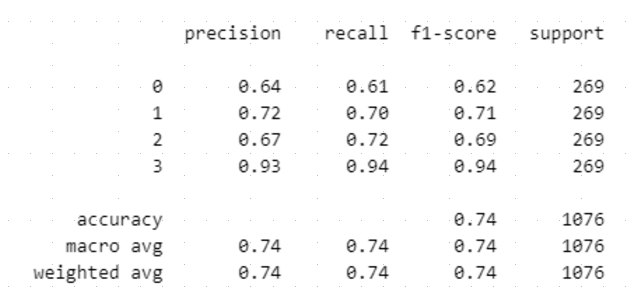
\includegraphics[width=0.4\linewidth]{XGBoost_128_no_aug_mask_cf_report.png}}%
  \qquad
  \subfloat[][]{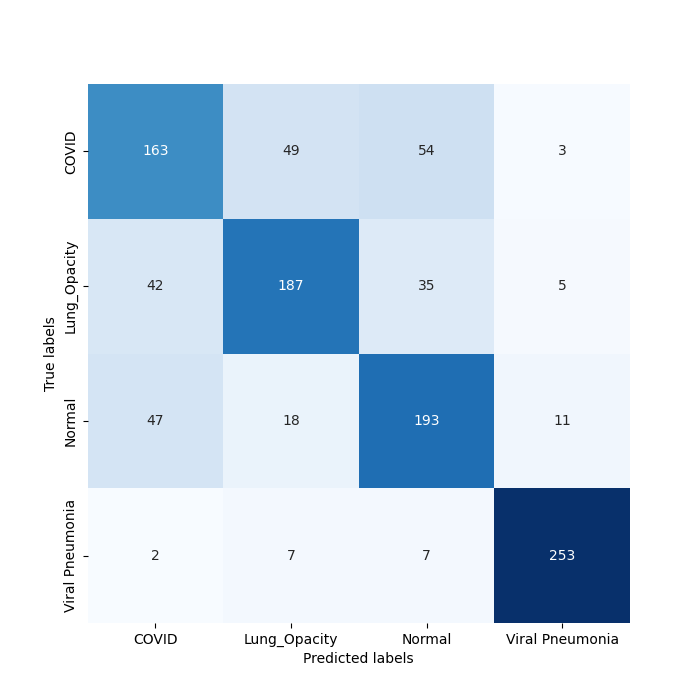
\includegraphics[width=0.4\linewidth]{XGBoost_128_no_aug_mask_cm_abs.png}}%
  \caption{XGBoost with 4000 images of size 128x128 pixels}
  \label{fig:XGBoost_128_no_aug_mask}
\end{figure}

Figure \ref{fig:XGBoost_128_no_aug_mask}a shows that the overall accuracy was 74\%. This accuracy is much higher than 57\% which the SVClinear model reached on
the same dataset (cf. figure \ref{fig:SVC_4000_128x128_bayes}). The classification report and aswell the confusion matrix in figure \ref{fig:XGBoost_128_no_aug_mask}b 
show that the XGBoost model, like the SVClinear model, best predicts the class "Viral Pneumonia" (3), 
but with a f1-score of 94\% instead of only 83\%. XGBoost does a better prediction for the class "COVID" (0) with a f1-score of 62\% compared to the SVClinear model
with only a f1-score of 44\%. But a f1-score of 62\% is still not very satisfactory. Further tests e.g. with the entire dataset are needed. 

\textbf{2nd trial} - XGBoost (128 x 128, all images incl. augmentation, with masks)\\
As a next test we tried to increase the number of images used for modelling. As input data we used all the images still with a reduced size of 128x128 pixels. 
To these images all preprocessing steps from \ref{preprocessing_pipeline} apart from feature extraction have been apllied.\\
As the first trial with XGBoost already showed, that we did not need 5000 "number of boost rounds" we reduced it in this test to 500 and additionally kept on 
using the early stopping technique. \\
Figure \ref{fig:XGBost_classifier_method_128_mask} shows that the overall accuracy is nearly the same as in the previous test where we used only 4000 non-augmented 
images. The f1-score for the "COVID class" (0) is with 57\% even a bit lower. But for the other classes the f1-score increased compared to the first test with XGBoost.\\

\begin{figure}[!ht]
  \centering
  \subfloat[][]{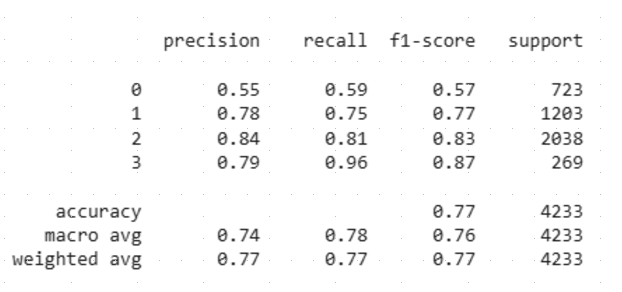
\includegraphics[width=0.4\linewidth]{XGBost_classifier_method_128_mask_cf_report.png}}%
  \qquad
  \subfloat[][]{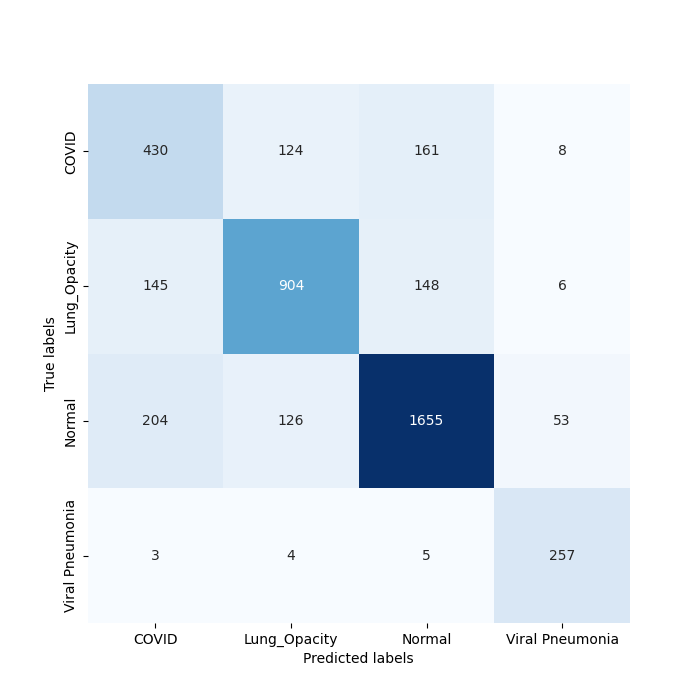
\includegraphics[width=0.4\linewidth]{XGBost_classifier_method_128_mask_cm_abs.png}}%
  \caption{XGBoost with all images of size 128x128 pixels, with masks}
  \label{fig:XGBost_classifier_method_128_mask}
\end{figure}



\textbf{3rd trial} - XGBoost (128 x 128,HOG-features)\\
For this test we tried to use the HOG-extracted features as input data. The classification report in figure \ref{fig:XGBost_hog}a  and the confusion matrix
in figure \ref{fig:XGBost_hog}b show that this did not improve the accuracy of 77\% and still the "COVID class" (0) is not predicted very well with a f1-score of
only 57\%.

\begin{figure}[!ht]
  \centering
  \subfloat[][]{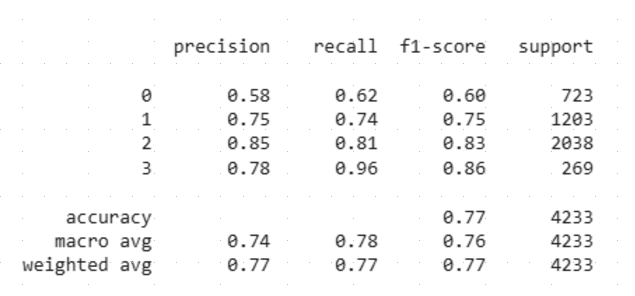
\includegraphics[width=0.4\linewidth]{XGBost_classifier_method_hog_cf_report.png}}%
  \qquad
  \subfloat[][]{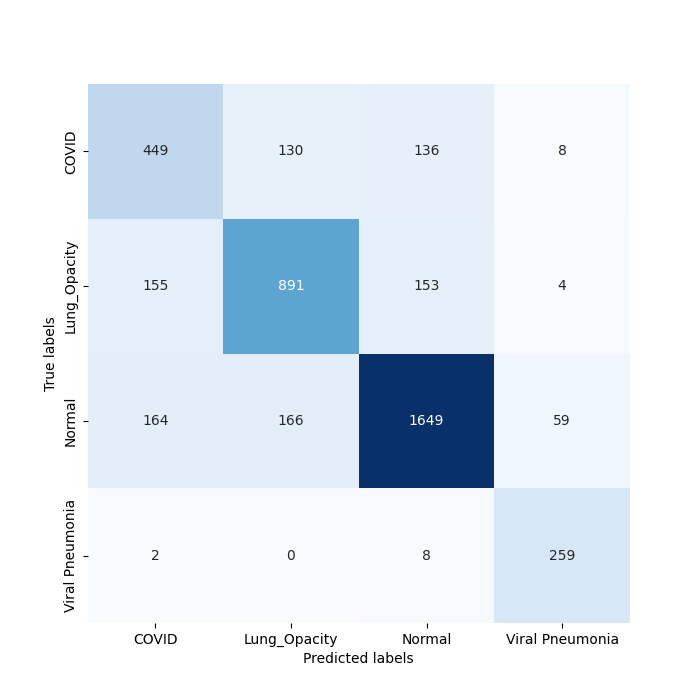
\includegraphics[width=0.4\linewidth]{XGBost_classifier_method_hog_cm_abs.png}}%
  \caption{XGBoost using hog features}
  \label{fig:XGBost_hog}
\end{figure}

\textbf{4th trial} - XGBoost (128 x 128, all images, without masks, no filter (Clahe, Gaussian Blur))\\
As a next step we tried to stick to use a big number of images and used all images inclduing the augmented images as input data. The images have been normalized but
no filters and masks were applied. \\
The classification report in figure \ref{fig:XGBost_classifier_method_128_nomask_nofilter}a and the confusion matrix in figure 
\ref{fig:XGBost_classifier_method_128_nomask_nofilter}b show that this model has an overall accuracy of 86\% which is the best accuracy of all XGBoost models we 
tried so far. This model can even predict the "COVID class" quiet good with a f1-score of 89\%. The worst f1-score has the "Lung-Opacity class" (1), with still 81%.\\
There are two options which change in the input data could have made this improvement compared to the previous tests: using no masks or using no filters. 

\begin{figure}[!ht]
  \centering
  \subfloat[][]{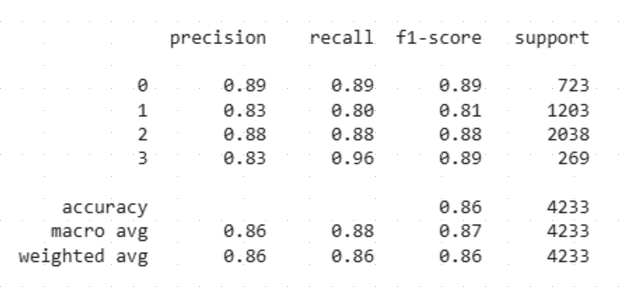
\includegraphics[width=0.4\linewidth]{XGBost_classifier_method_128_nomask_cf_report.png}}%
  \qquad
  \subfloat[][]{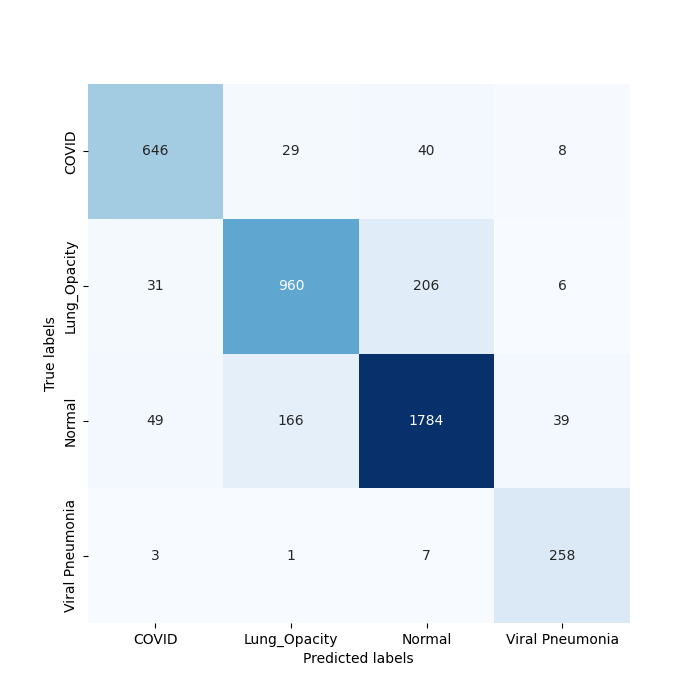
\includegraphics[width=0.4\linewidth]{XGBost_classifier_method_128_nomask_cm_abs.png}}%
  \caption{XGBoost with all images of size 128x128 pixels, without masks, no filters}
  \label{fig:XGBost_classifier_method_128_nomask_nofilter}
\end{figure}



\textbf{5th trial} - XGBoost (128 x 128, all images, without masks, WITH filters (Clahe, Gaussian Blur))\\
As a conclusion of the previous test (4th trial) we tried to use the same input data but this time using filters. The classification report in 
figure \ref{fig:XGBost_classifier_method_128_nomask_withfilter}a and the confusion matrix in figure \ref{fig:XGBost_classifier_method_128_nomask_withfilter}b show
that using the filters reduced the overall accuracy a bit to 85\% and also the f1-score for the "COVID class" (0) is only 84\% instead of 89\% as in the 
test without filters. 

\begin{figure}[!ht]
  \centering
  \subfloat[][]{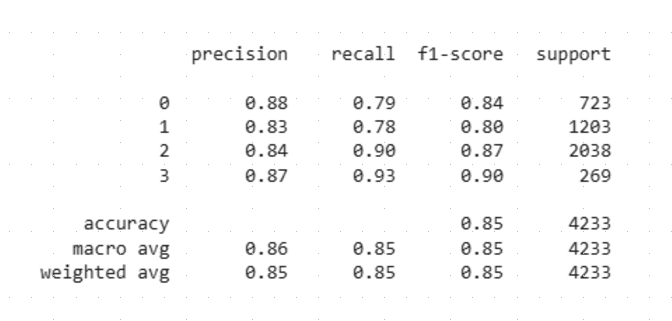
\includegraphics[width=0.4\linewidth]{XGBost_classifier_method_128_nomask_filters_cf_report.png}}%
  \qquad
  \subfloat[][]{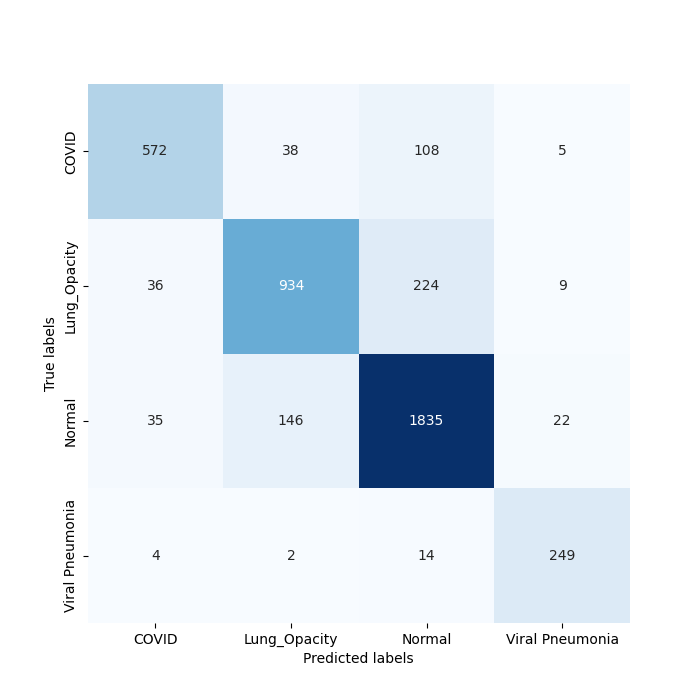
\includegraphics[width=0.4\linewidth]{XGBost_classifier_method_128_nomask_filters_cm_abs.png}}%
  \caption{XGBoost with all images of size 128x128 pixels, without masks, with filters}
  \label{fig:XGBost_classifier_method_128_nomask_withfilter}
\end{figure}

As a next test we could try using masks and no filters. But as time in this project is reduced we moved on to using deep learning models which looks 
more promising when working with images. 

\subsubsection {MLP-Classifier} 
Multi-Layer Perceptron, which is a classic feedforward neural network consists of: An input layer, One or more hidden layers (each with fully connected / dense neurons) and an output layer. Each neuron in a layer is connected to every neuron in the next layer which makes it a dense network.\\
 
\textbf{1st trial}\\We trained an MLPClassifier (Multi-layer Perceptron) using HOG features. The first MLP classsifer had the following architecture: sequential 3 dense layers: 512, 256, 128 neurons, ReLU activation + dropout, model compiled using adam optimizer and categorical crossentropy loss. This gave us solid result for a first MLP on HOG features — 78\% accuracy with especially strong recall on Viral Pneumonia (97\%).
In the next trial we improved this further by making improvements to the model architecture.\\

\textbf{2nd trial}\\
We increased the number of layers/neurons to make deeper network (Sequential layers: 1024, 512, 256)
and performed BatchNormalization before activations for more stable training, implemented EarlyStopping + ReduceLROnPlateau for smarter training.
The overall accuracy of this model was 76.99 \%, which is a notable boost from previous models. However, COVID (0) is still the weakest class (59\% precision and recall), indicating the model struggles with it — possibly due to class imbalance or feature overlap. Lung Opacity (1) shows consistent, decent performance (75\% recall). Normal (2) displayed the strongest precision (85\%) and recall (82\%), showing good separability. Viral Pneumonia (3) displayed excellent recall (96\%) as it had very few false negatives.\\

\textbf{3rd trial}\\
The next trial  we tried an updated MLP classifier with an edition of Class weights to Boost minority class (COVID) explicitly, and activation function Leaky Relu to avoid dead neurons, in addition to previous additions. The key changes made were:
 \begin{itemize}
     \item LeakyReLU with alpha=0.1 helps mitigate dead neurons by allowing a small gradient when the input is negative.
     \item Dropout with rates of 50\% after the first layer and 30\% after the second layer helps prevent overfitting by randomly dropping out neurons during training.
     \item Adam optimizer with a smaller learning rate (0.0005) to help avoid overshooting the minima during training.
     \item Class weights are computed to handle class imbalance (especially important for class 0 - COVID).
     \item Batch Normalization is included after each layer to stabilize the learning process
\end{itemize}
The accuracy is now 0.7817, which is a noticeable improvement from the previous attempts. Looking at the confusion matrix, we can observe: Class 0 (COVID) has lower precision and recall than the other classes. This could mean our model is having difficulty distinguishing between COVID and other classes (maybe due to class imbalance). Classes 1 (Lung Opacity), 2 (Normal), and 3 (Viral Pneumonia) are being classified well, with high F1-scores and balanced precision and recall.\\

\textbf{4th trial}\\
In this model we appliesd SMOTE to help balance the class distribution by generating synthetic samples for the minority classes (Class 0 - COVID), which can help the model learn better representations for those classes.We later scaled the resampled features using 50 epochs, Smaller batch size (32), early stopping, to prevent overfitting, and trained the model on the new balanced data (without class weights). Although the model gave consistent ~77.7–78\% accuracy, we observed good precision and recall for class 2 and 3 however class 0 is still underperforming.\\

\textbf{5th trial}\\
In this model we tried focal loss which is particularly useful when we're dealing with class imbalance, as it puts more focus on hard-to-classify examples.We used a gamma of 2.0 and alpha of 0.25 — good defaults based on the original focal loss paper. Class 0 is still underperforming slightly (precision = 0.60, recall = 0.58), meaning it's being confused with other classes. This is likely due to it having fewer or noisier samples or its features overlapping with class 1.Class 2 and 3 are performing very well, especially class 3 (recall = 0.93) — so the model is confidently identifying these.\\

\textbf{6th trial}\\
We next tried MLP on ResNet features.ResNet (Residual Networks) is a deep convolutional neural network pretrained on ImageNet.It learns hierarchical, high-level features (like textures, shapes, patterns) that are often more effective than handcrafted ones.Extracting features from a pretrained ResNet and feeding them into a simple MLP can boost performance, especially for medical images.
The model performed very well with an overall Accuracy of 82.8\%, COVID Recall: 69\%, Lung Opacity Recall: 78\%,    Normal Recall: 89\%,Pneumonia Recall: 94\%.This matrix shows that:Normal and Pneumonia classes are classified with high confidence. COVID and Lung Opacity occasionally get confused with each other and with Normal.
Our current results are strong enough that it makes perfect sense to move to deep learning or CNN-based models next.
\begin{figure}[ht] % the [h!] helps force it "here"
    \centering
    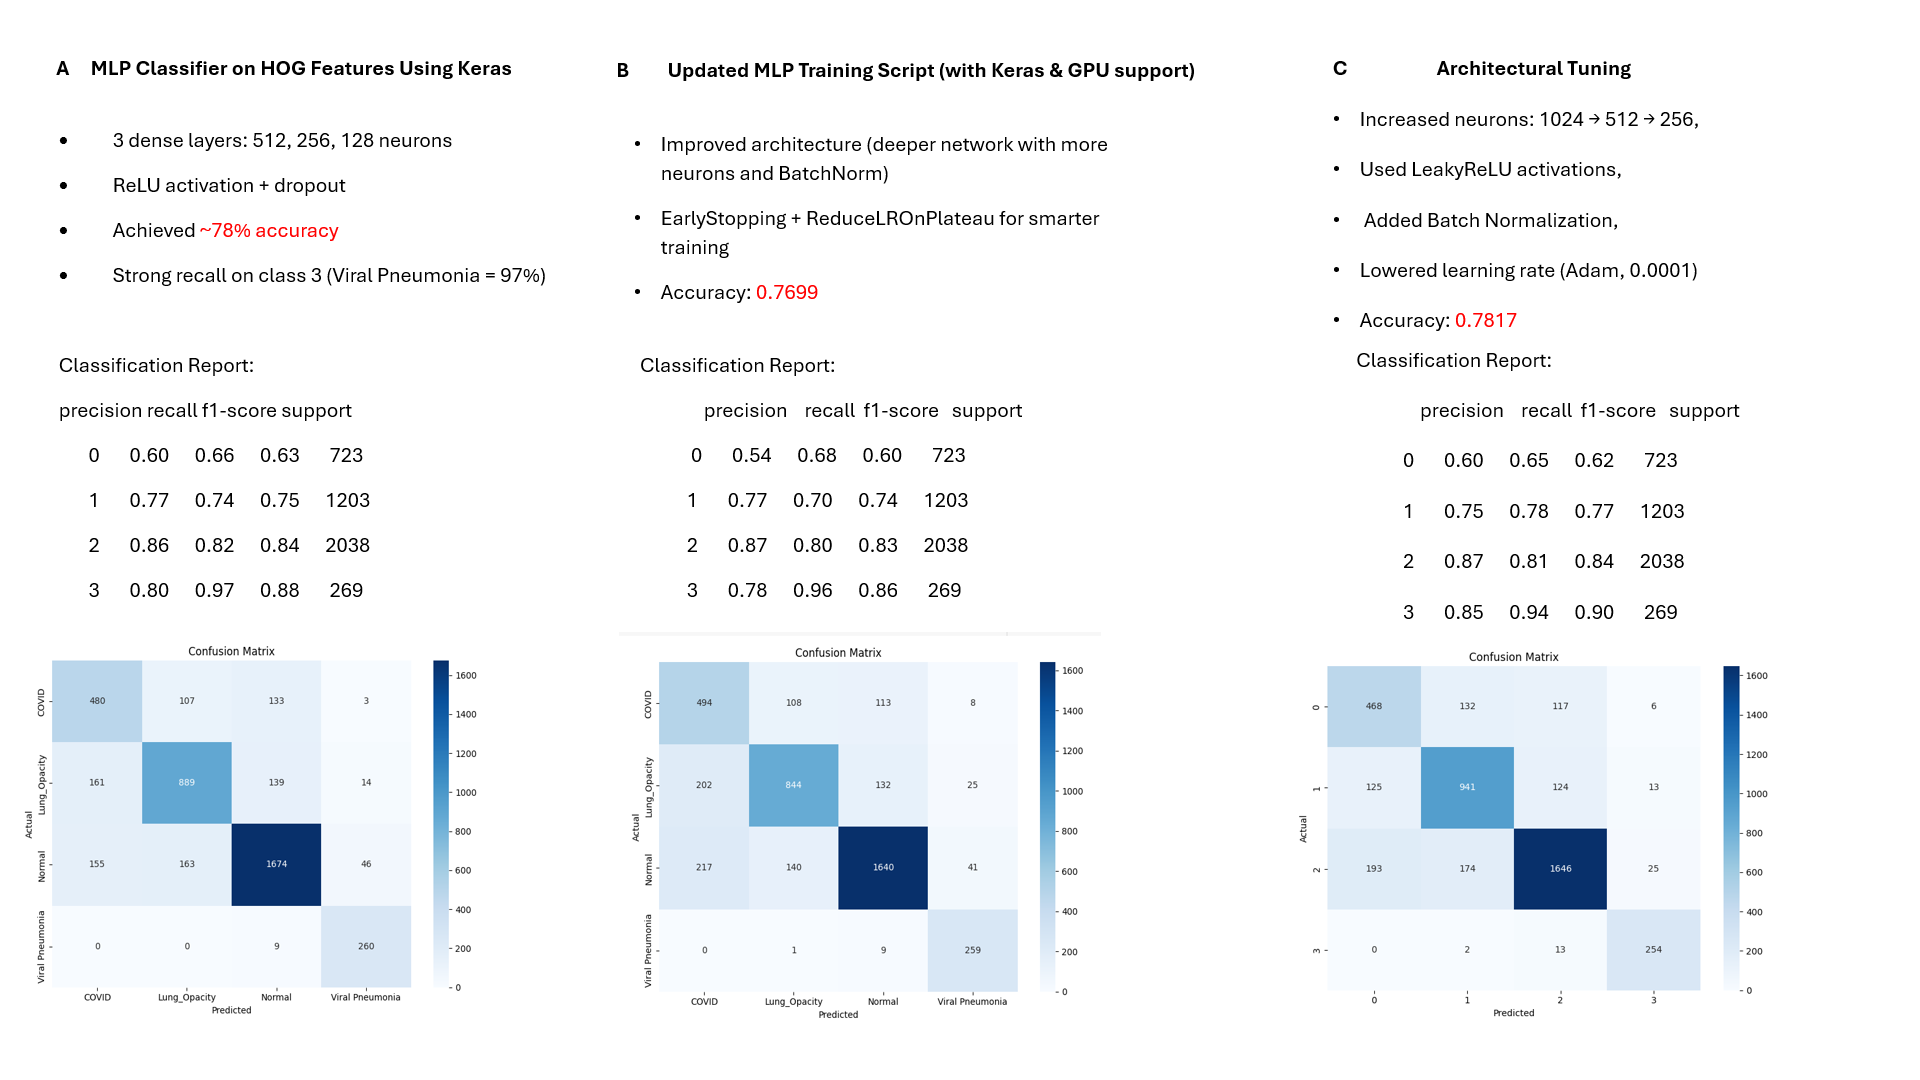
\includegraphics[width=1.0\linewidth]{mlpclassifier a,b,c.png}
    \caption{MLP CLASSIFIER A, B, C}
    \label{fig:MLP_CLASSIFIER}
\end{figure}
We wanted to see how the MLP classifier model was learning our data anad so we decided to plot the accuracy and loss per epochs for the first trial and the last (figure \ref{fig:MLP_CLASSIFIER_compare}). On analysis of figure \ref{fig:MLP_CLASSIFIER_compare}a (20 epochs) we found training Loss decreases steadily suggesting the model is learning from the training data.
The Validation Loss Plateaus and then increases after epoch ~6–7 which suggests overfitting.The model training Accuracy rises to ~0.95 which is excellent however the validation Accuracy flatlines around 0.83–0.84 which showed that the model is not improving on unseen data.
Figure \ref{fig:MLP_CLASSIFIER_compare}b (8 epochs) showed a similar trend, just shorter duration. We obeserved still a gap between training and validation performance (train ~0.93 vs val ~0.83).The validation loss increases even earlier suggesting overfitting happens faster.\\
These resulsts show that Resnet features wrok well and MLP learns effectively on the training data.However, we observe overfitting whih needs to be fixed.\\
\textbf{7th trial}\\
To address this we next try to add L2 regularization to Dense layers that helps reduce overfitting by penalizing large weights, increase dropout slightly (0.4) that increases regularization by randomly dropping neurons during training and use early stopping that avoids overfitting by halting training when the model stops improving on validation data.We also try reducing the number of neurons (e.g., 256 → 128 → 64) to avoid overfitting and consider adding BatchNormalization after dense layers.
\begin{figure}[ht] % the [h!] helps force it "here"
    \centering
    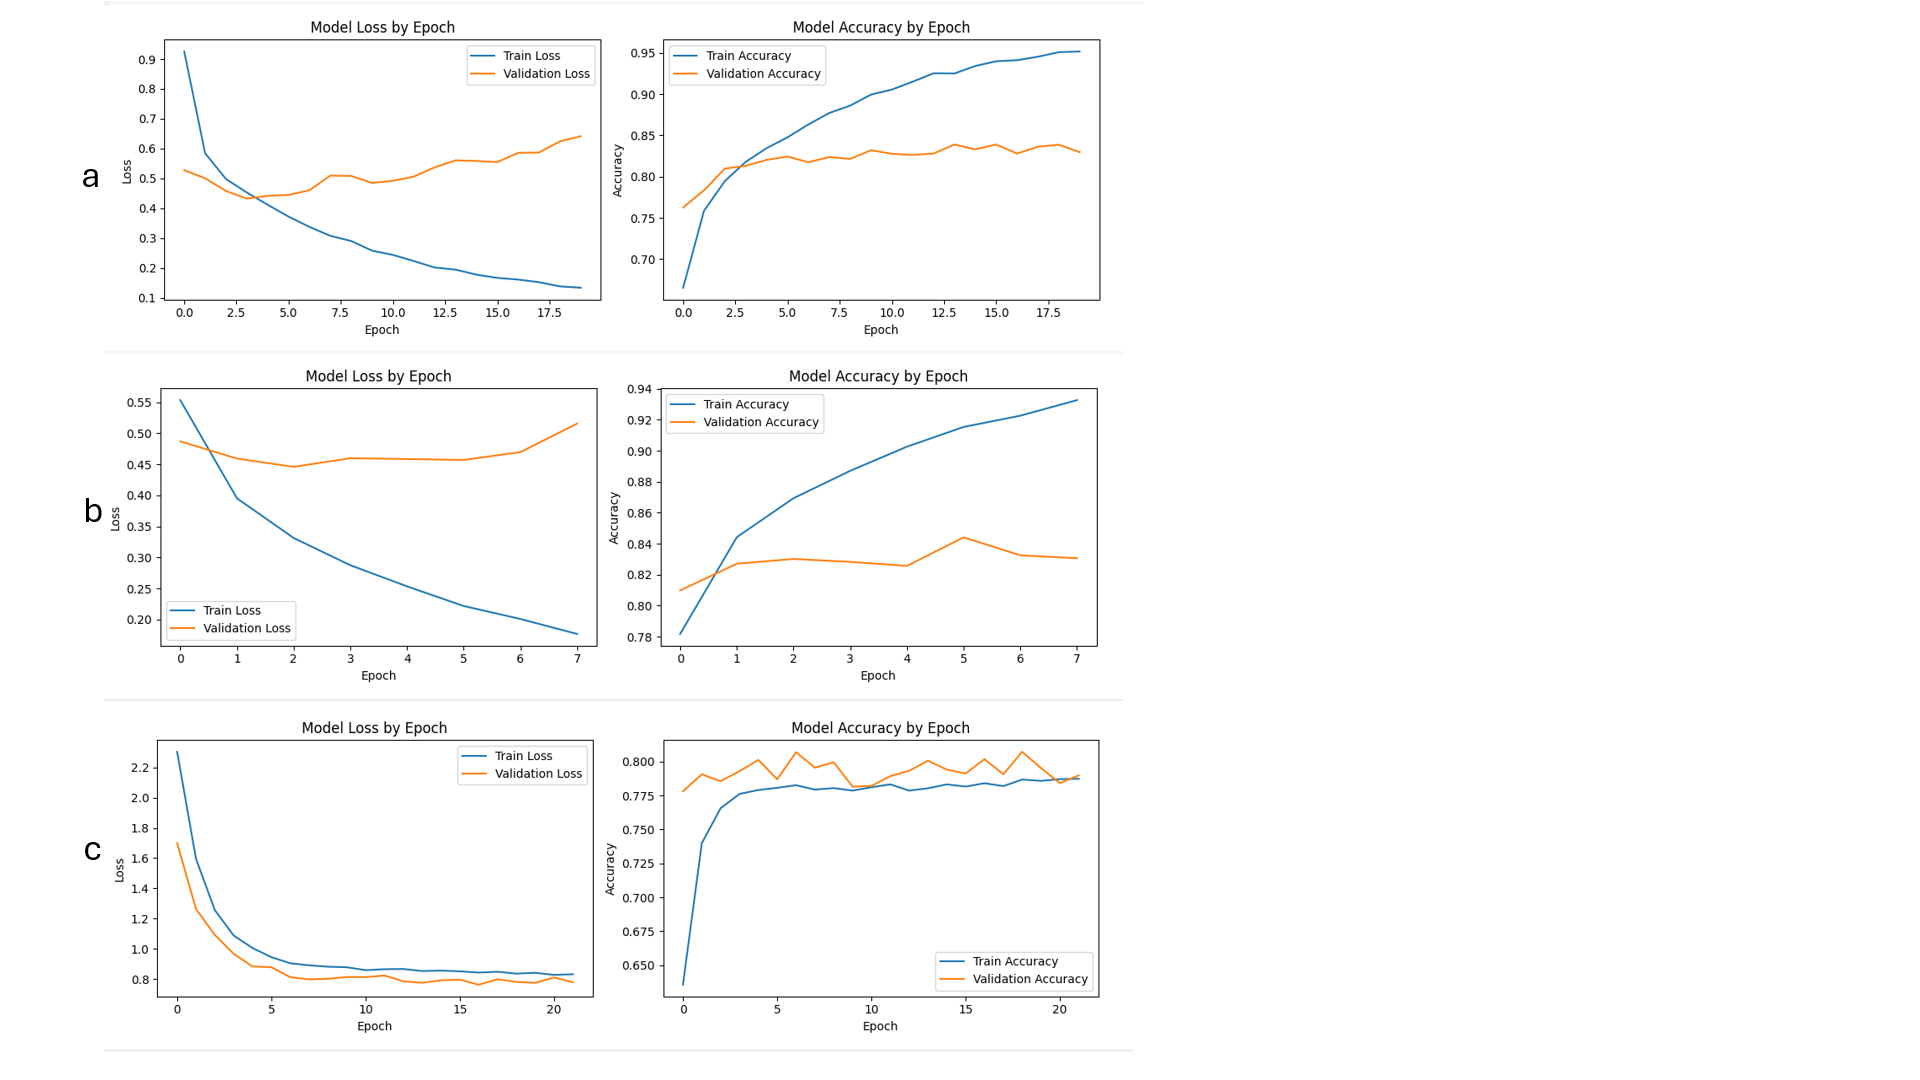
\includegraphics[width=1.0\linewidth]{comparemlp2.png}
    \caption{MLP CLASSIFIER A, B, C}
    \label{fig:MLP_CLASSIFIER_compare}
\end{figure}
Loss and Accuracy Plot Interpretation of figure \ref{fig:MLP_CLASSIFIER_compare}c shows that both training and validation loss drop significantly in the first few epochs and stabilize around epoch 10.The gap between training and validation loss is small, which means low overfitting.Accuracy rises quickly and stabilizes around 78–80\% for both training and validation, showing consistent learning and generalization.
The validation accuracy occasionally surpasses training accuracy, likely due to dropout and regularization.

The Classification Report showed an overall accuracy of 75\% over 4,233 samples which is solid for a multi-class task.
Class 2 (largest class): Strong performance (F1 = 0.83), suggesting the model is very confident in this class.
Class 1: Also good (F1 = 0.72).
Class 0: Weaker (F1 = 0.56), possibly due to overlapping features.
Class 3: Interesting — high recall (0.98) but lower precision, suggesting the model predicts this class a lot, possibly overgeneralizing to it.\\
\\
In conclusion, MLP Classifier on ResNet Features gave us the best accuracy(82\%).Since class 0 still remians a probelm moving to a Convolutional Neural Network (CNN) is the logical next step, since were working with image data (X-rays), and traditional ML models like SVMs or MLPs (even with augmentation and tuning) may struggle to capture spatial hierarchies and localized patterns critical for medical imaging.\\

\section{Deep Learning}

\subsection{Prepare Data for Deep Learning}
When trying to train different deep learning models, we figured out that we had to play around with the data. We tried different pre-preprocessing steps for the different models. Therefore, the different pre-processing steps are described in the respective chapters of the deep learning models.

\subsection{Metrics to Evaluate the Model Results}
For the evaluation of the results of the deep learning models, we used the same methods (classification report, confusion matrix) as for the evaluation of the machine learning models, c.f. section \ref{metrics_ML}. \\
Additionally, we analyzed how the accuracy and the loss evolved over the different epochs. \\
For some models we wanted to visualize which areas of an image contribute most to a model's decision. Therefore, we used Grad-CAM whether the model is paying attention to relevant anatomical features in the X-ray images.
\subsection{Convolutional Neural Networks}
\subsubsection{Self-built CNN}
With X-ray images, CNNs are still very strong, but transformers can outperform them.
We built a CNN model for image classification, with three convolutional blocks for feature extraction, followed by pooling, dense layers for classification, and dropout for regularization.
\paragraph{Data pre-processing for CNN}\mbox{}\\
The data preparation for training the CNN model on the COVID-19 Radiography Database involved several steps. First, the dataset was downloaded from Kaggle using the Kaggle API and extracted. This dataset contains chest X-ray images categorized into four classes: Normal, COVID, Lung\_Opacity, and Viral Pneumonia. Each class folder includes both the raw images and corresponding segmentation masks highlighting lung regions. The data was then split into training and testing sets using an 85:15 ratio, ensuring that both images and their associated masks were kept aligned. These were organized into a structured directory format under separate folders for training and testing data, with further subdivisions by class and file type (images or masks).

For model input preparation, both images and masks were resized to 224×224 pixels. Each grayscale image was normalized to a [0, 1] range and then multiplied pixel-wise with its mask to retain only the lung regions, effectively focusing the model’s attention. The processed grayscale image was duplicated across three channels (to match expected RGB input format), and the mask was added as a fourth channel—resulting in a 4-channel input tensor. Data augmentation, using the Albumentations library, was selectively applied to minority classes (those with fewer samples) to mitigate class imbalance. These augmentations included horizontal flips, small rotations, shifts, and scaling.

Finally, the processed data was loaded into TensorFlow datasets using a generator-based pipeline, yielding batches of 4-channel images with their corresponding class labels. These datasets were shuffled, batched, and prefetched to ensure efficient training. This pipeline ensured that the model could learn not only from image features but also leverage the spatial context provided by lung masks, thereby improving classification accuracy on chest X-rays.


Table \ref{tab:cnn_architecture} shows the reasons for the cnn architecture :
\begin{table}[h]
    \centering
    \renewcommand{\arraystretch}{1.3}
    \begin{tabular}{|c|c|p{8cm}|}
        \hline
        \textbf{Component} & \textbf{Purpose} \\ \hline
        Conv2D layers & Extract spatial features from images \\ \hline
        BatchNorm & Normalize for stability and faster convergence \\ \hline
        ReLU & Introduce non-linearity to learn complex patterns \\ \hline
        MaxPooling2D & Downsample to reduce spatial size and computation \\ \hline
        GlobalAvgPooling & Reduce 2D maps to 1D vector without flattening full feature map \\ \hline
        Dense + Dropout & Learn final abstract representations and prevent overfitting \\ \hline
        Softmax Output	& Multiclass classification probabilities \\ \hline
    \end{tabular}
    \caption{Comparison of hyperparameter tuning strategies}
    \label{tab:cnn_architecture}
\end{table}
\paragraph{The CNN Model}\mbox{}\\
Figure \ref{fig:model_cnnmask1.keras.png} shows the architecture of our model

\begin{itemize}
    \item Input: The input for our model was 4-channel images of shape (Height, Width, 4), where the 4 channels were  RGB + mask.
    \item Conv Block 1: Conv2D (32 filters, 3x3, padding='same')learns low-level features (edges, blobs), BatchNormalization normalizes activations to stabilize and speed up training, Activation (ReLU) adds non-linearity.MaxPooling2D (2x2)downsamples feature maps (reduces spatial resolution).
    \item Conv Block 2:Conv2D (64 filters, 3x3, padding='same')learns more complex patterns, BatchNormalization, Activation (ReLU), MaxPooling2D (2x2)
    \item Conv Block 3:	Conv2D (128 filters, 3x3, padding='same')for even deeper features, BatchNormalization,	Activation (ReLU), MaxPooling2D (2x2)
    \item GlobalAveragePooling2D: Converts the spatial feature map into a 1D feature vector by averaging, Reduces parameters before entering dense layers,	Helps avoid overfitting and makes model more robust.
    \item Dense Layers (Fully Connected): Dense (256 units, ReLU), First FC layer with ReLU for learning abstract combinations of features, Dropout (rate=0.3) for Regularization to prevent overfitting, Dense (128 units, ReLU) for Smaller FC layer,	Dropout (rate=0.3) again helps generalize better.
    \item Output Layer:Dense (4 units, Softmax)Final output layer with 4 units = 4 classes, Softmax gives probability distribution over the classes.
\end{itemize}


\begin{figure}[h!] % the [h!] helps force it "here"
    \centering
    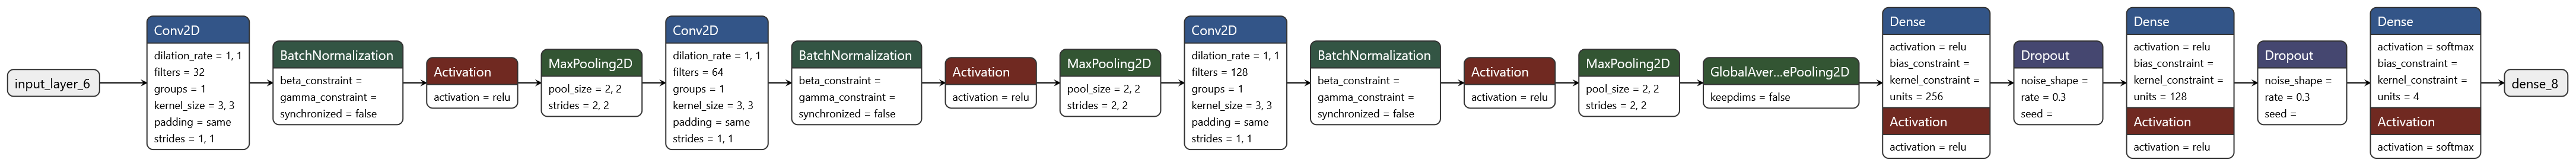
\includegraphics[width=1.0\linewidth]{model_cnnmask1.keras.png}
    \caption{CNN Architecture}
    \label{fig:model_cnnmask1.keras.png}
\end{figure}

The CNN model demonstrated strong performance on the chest X-ray classification task, as reflected in the classification report. Overall, the model achieved an accuracy of 92\% on the test set consisting of 3,598 images. When broken down by class, the model performed particularly well on the COVID and Viral Pneumonia categories. For COVID cases, it attained a precision of 93\%, a recall of 98\%, and an F1-score of 95\%, indicating both high correctness and sensitivity in identifying positive cases. Viral Pneumonia predictions were even more robust, with a precision of 96\%, recall of 98\%, and an F1-score of 97\%. The model also performed well on the Normal class, achieving a precision of 91\% and a recall of 96\%. The Lung Opacity class posed more of a challenge, with a slightly lower recall of 82\%, though precision remained high at 93\%, yielding an F1-score of 87\%. The macro and weighted averages across all classes were both around 93\% for precision, recall, and F1-score, underscoring the model’s balanced performance across a multi-class classification task.
We can see the confusion matrix and the classification report for our model in figure \ref{fig:cnn_results.png}.

\begin{figure}[h!] % the [h!] helps force it "here"
    \centering
    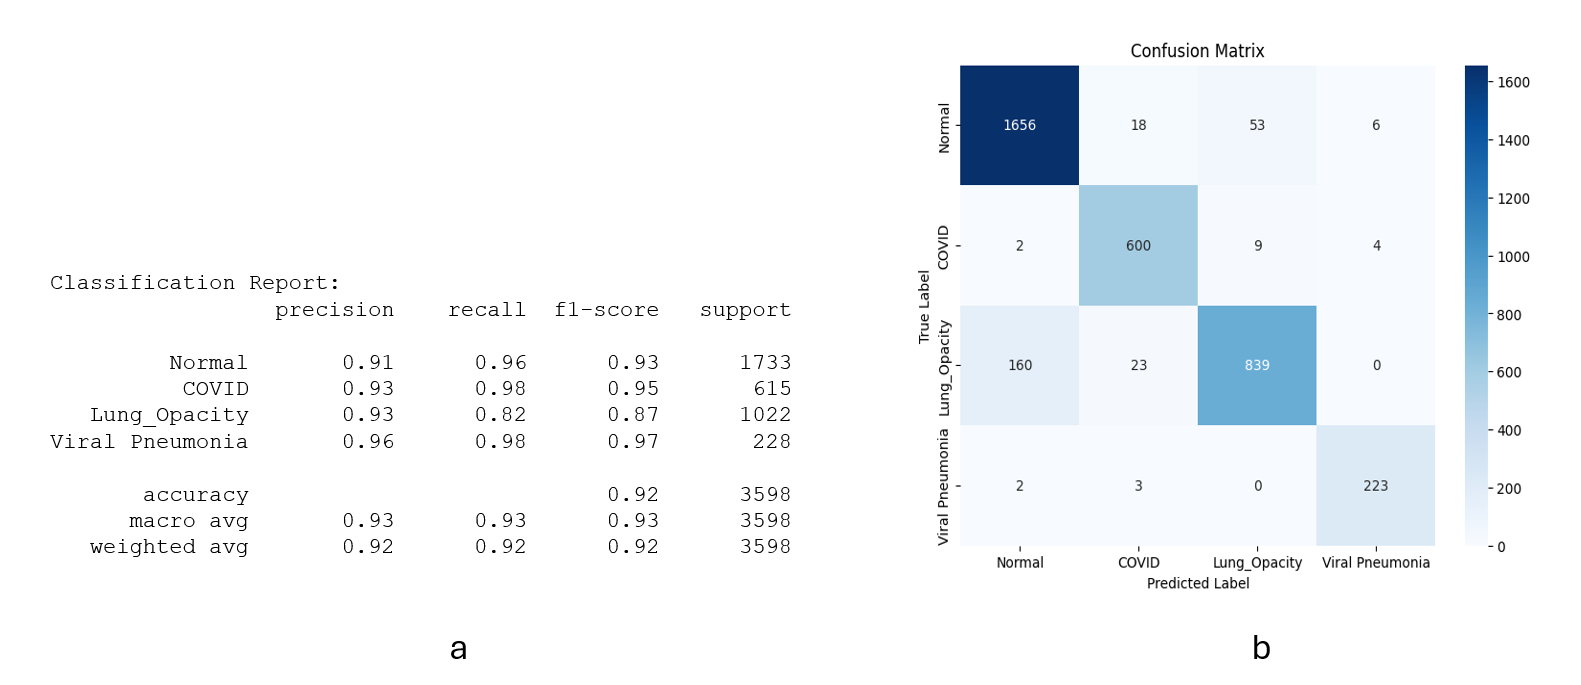
\includegraphics[width=1.0\linewidth]{cnn results.png}
    \caption{CNN Results}
    \label{fig:cnn_results.png}
\end{figure}

\subsection{Using pretrained models with transfer learning}

\subsubsection{VGG16}
\paragraph{First Trial: Offline Feature Extraction + Separate Classifier}\mbox{}\\
In our model we used a fully connected Deep Neural Network (DNN) classifier. 

\begin{figure}[h!] % the [h!] helps force it "here"
    \centering
    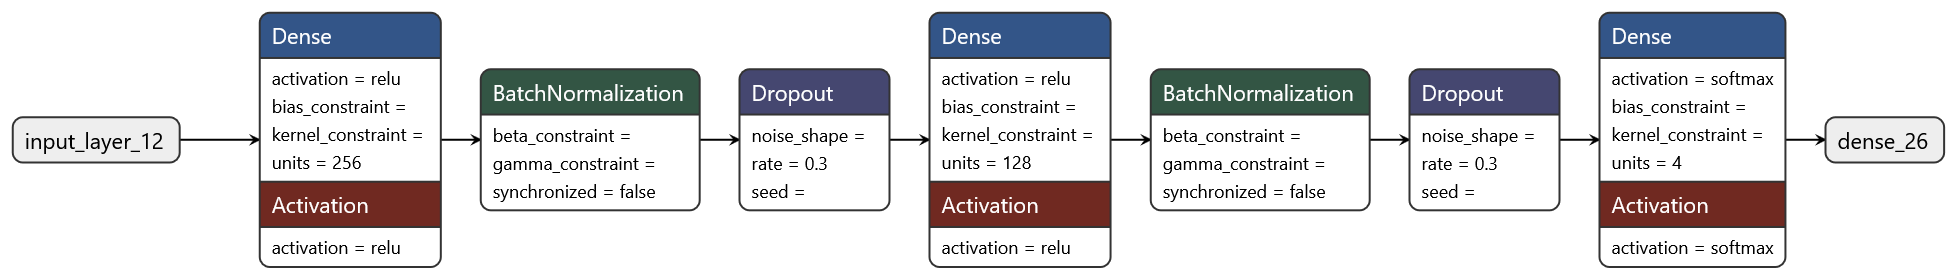
\includegraphics[width=1.0\linewidth]{vgg16_model1.keras(1).png}
    \caption{CNN Results}
    \label{fig:vgg16offlinemodel.png}
\end{figure}
In this workflow, figure \ref{fig:vgg16offlinemodel.png}., we utilize a hybrid deep learning approach by leveraging pretrained VGG16 features for efficient image classification. First, grayscale medical images are converted to RGB, resized to 224×224, and passed through the VGG16 model (with include\_top=False and global average pooling) to extract compact 512-dimensional feature vectors. These features are precomputed and saved for training, validation, and testing datasets. Instead of retraining the entire VGG16 model, we then build a lightweight, fully connected neural network that takes these feature vectors as input. The classifier consists of dense layers with ReLU activation, batch normalization, dropout for regularization, and a final softmax layer to predict one of four classes. Additionally, input features are standardized using StandardScaler to improve training stability.

\begin{figure}[h!] % the [h!] helps force it "here"
    \centering
    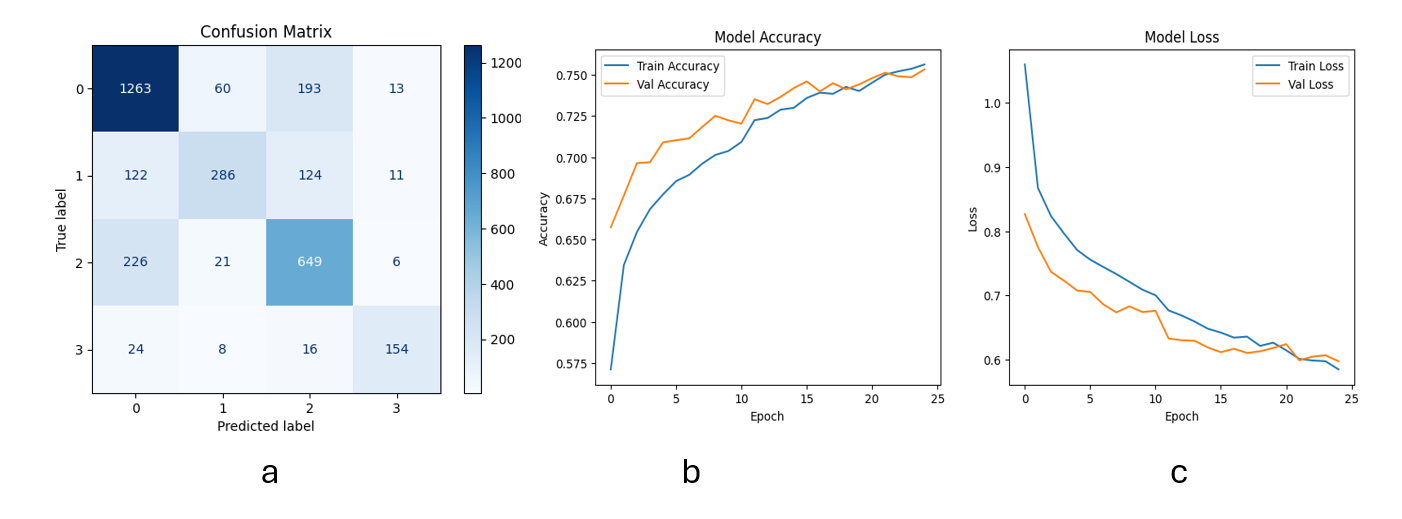
\includegraphics[width=1.0\linewidth]{vgg16_offlinetransfer.png}
    \caption{Results for VGG offline transfer}
    \label{fig:vgg16offlineresults.png}
\end{figure}

This trial model gave us an accuracy of 77\% (figure \ref{fig:vgg16offlineresults.png}) and was computationally cost-efficient while retaining the representational power of deep features learned from ImageNet.Therefore, we next decided to perform online transfer learning using the VGG16 model.
\paragraph{Second Trial: Online Transfer Learning Using VGG16}\mbox{}\\
\paragraph{Data pre-processing for CNN}\mbox{}\\
 For this grayscale chest X-ray images are first organized and preprocessed effectively. The dataset is split into training and validation sets class-wise (Normal, COVID, Lung Opacity, Viral Pneumonia) with corresponding segmentation masks, and further balanced using data augmentation. Each image is converted from grayscale to RGB format by stacking the single channel, resized to 224×224, and normalized to the [0,1] range to match the input format expected by VGG16. Augmentations like horizontal flipping, rotation, and scale-shifting are selectively applied to minority classes to mitigate class imbalance. A custom TensorFlow tf.data.Dataset pipeline efficiently streams the data in batches with prefetching for GPU acceleration, allowing VGG16 to learn meaningful features directly from image batches without prior feature extraction. This preparation ensures the model benefits from both the pretrained representations of VGG16 and the robustness offered by dynamic, on-the-fly data augmentation.
Figure \ref{fig:vgg16augmentations.png} shows a batch we visualized to ensure only minority class images are augmentated.
\begin{figure}[h!] % the [h!] helps force it "here"
    \centering
    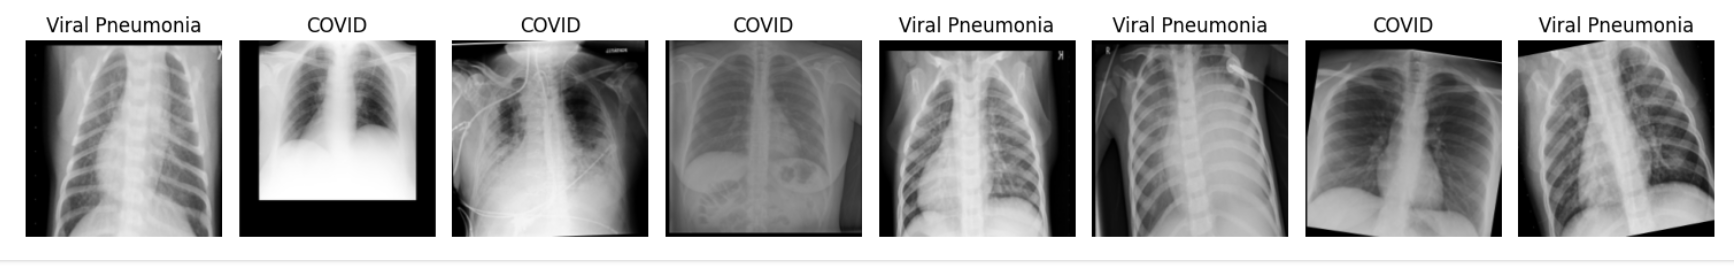
\includegraphics[width=1.0\linewidth]{vgg16augmentations.png}
    \caption{VGG augmentations}
    \label{fig:vgg16augmentations.png}
\end{figure}
\paragraph{Model preparation}\mbox{}\\
In this trial, an online feature extraction approach was implemented using the pretrained VGG16 model from the ImageNet dataset. The convolutional base of VGG16 was used as a fixed feature extractor by freezing its layers (`trainable = False`), allowing only the custom classification head to be trained. The input images, resized to 224×224×3, were passed through the VGG16 base, followed by a classification head composed of a `GlobalAveragePooling2D` layer, two fully connected (`Dense`) layers with ReLU activations, and `Dropout` layers to reduce overfitting. The final output layer used a softmax activation to predict one of four target classes. The model was compiled with the Adam optimizer and trained for 5 epochs using sparse categorical crossentropy as the loss function. The training utilized TensorFlow data generators created from the augmented dataset, with training and validation steps computed based on the batch size and dataset size. This setup allowed end-to-end learning of high-level features while leveraging the robustness of pretrained weights.
\begin{figure}[h!] % the [h!] helps force it "here"
    \centering
    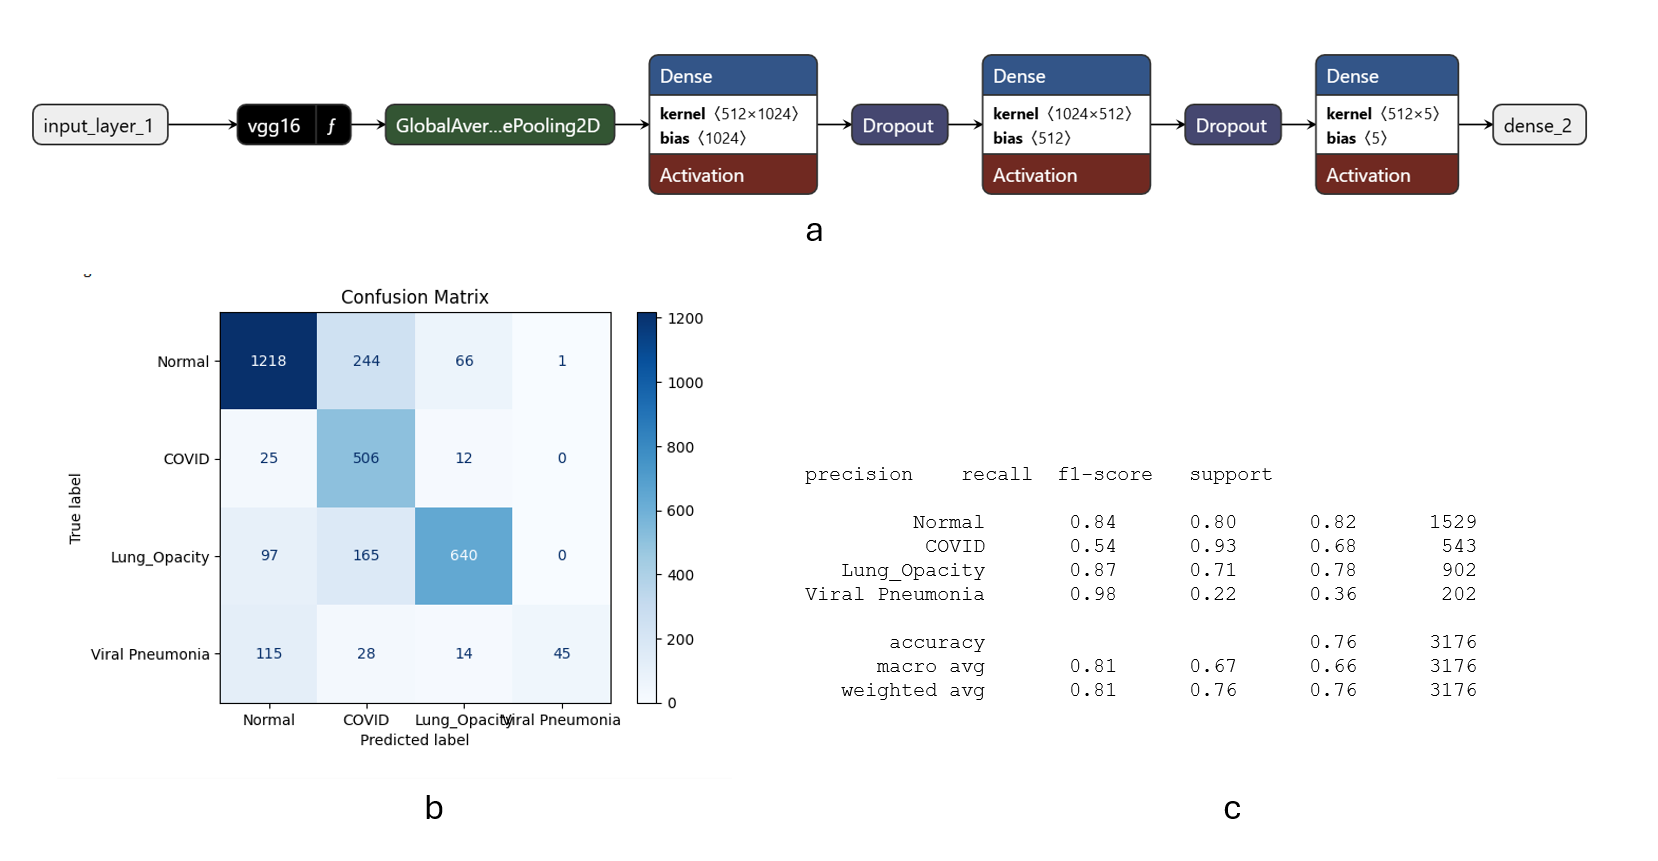
\includegraphics[width=1.0\linewidth]{vgg16online1.png}
    \caption{Model Archtecture and Results for second trial using VGG 16 online transfer}
    \label{fig:vgg16result1.png}
\end{figure}
Figure \ref{fig:vgg16result1.png} shows the architecture of the model used and the confusion matirx and the classification report for the model training.The evaluation results of the model reveal a moderate overall performance, achieving an accuracy of 76\% across the four classes. The Normal and Lung Opacity classes performed well, with F1-scores of 0.82 and 0.78, respectively, indicating balanced precision and recall. The model demonstrated excellent recall for the COVID class (0.93), meaning it correctly identified most COVID cases, though the precision was lower (0.54), suggesting a higher number of false positives. Conversely, Viral Pneumonia showed poor performance, with a low recall of 0.22 despite a high precision of 0.98, indicating that while the few predictions made were mostly correct, the model failed to identify the majority of these cases. The macro average F1-score of 0.66 reflects this imbalance across classes, while the weighted average F1-score of 0.76 suggests the model was skewed toward better performance on more frequent classes. These results highlight the need for improvements in model capacity or training strategy to achieve more balanced performance.

\paragraph{Third Trial: Fine-tuning VGG16 Transfer Model : Unfreeze last 4 layers}\mbox{}\\
To enhance the performance of the VGG16-based classifier, we transitioned from using a completely frozen base model to a fine-tuned version by unfreezing the last four convolutional layers of the pretrained VGG16 architecture. This allowed the model to adapt more effectively to domain-specific features in chest radiographs while still retaining the benefits of transfer learning. The classification head remained the same, consisting of global average pooling followed by two fully connected layers with dropout regularization to reduce overfitting. We also reduced the learning rate to 1e-5 to prevent large updates that could disrupt the pretrained weights. Additionally, we incorporated callback functions such as `EarlyStopping` (to halt training if validation loss didn't improve) and `ReduceLROnPlateau` (to lower the learning rate dynamically during plateaus), promoting more stable and efficient training. These adjustments aimed to strike a balance between learning new task-specific representations and preserving useful pretrained knowledge.
\begin{figure}[h!] % the [h!] helps force it "here"
    \centering
    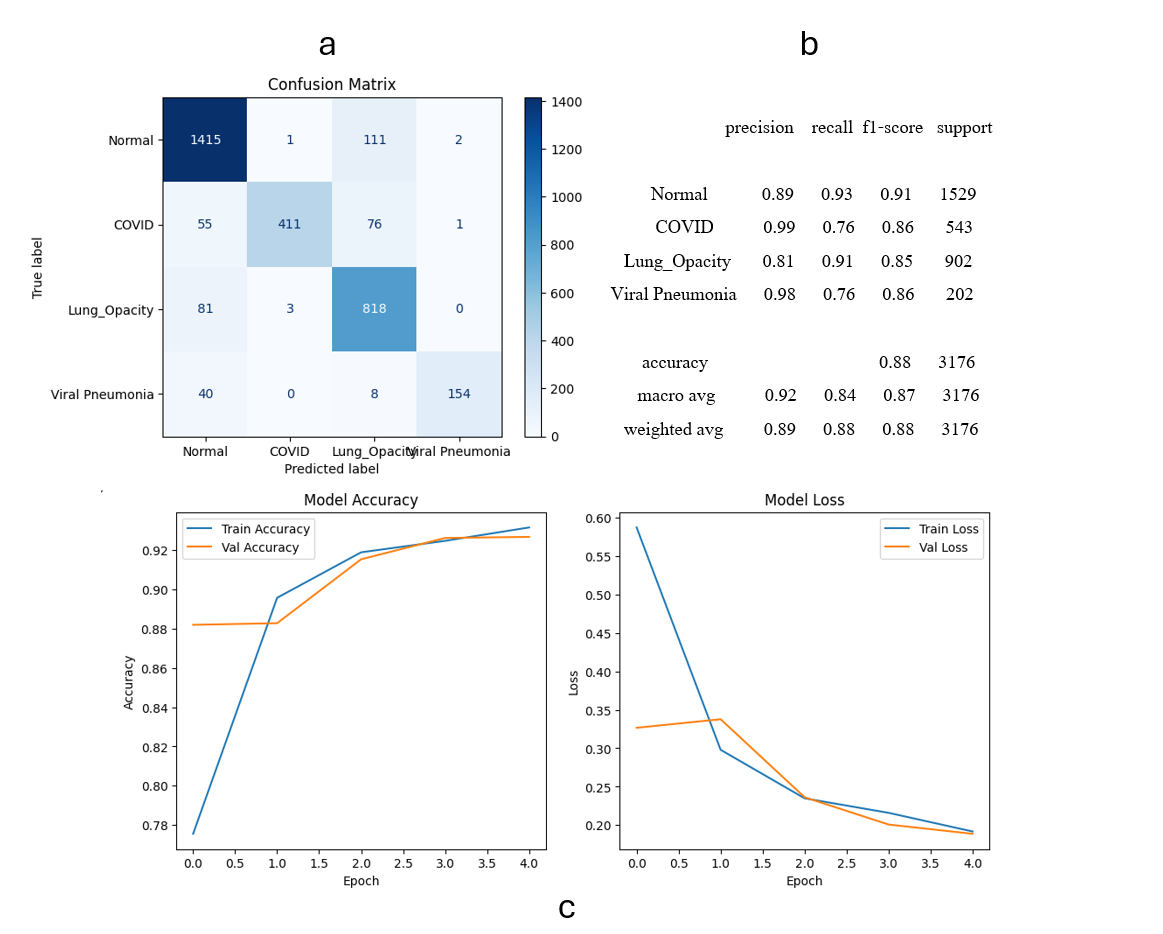
\includegraphics[width=1.0\linewidth]{vgg16-4.png}
    \caption{Results for third trial using VGG 16 (unfreeze last 4)}
    \label{fig:vgg16result2.png}
\end{figure}
Figure \ref{fig:vgg16result2.png} shows after unfreezing the last few layers of the VGG16 base and applying targeted training refinements, the model achieved a high overall accuracy of 88\% on the test set. Looking at the per-class performance, the model demonstrated strong precision and recall for the Normal class (precision: 0.89, recall: 0.93, F1-score: 0.91), indicating consistent detection of healthy chest images.
Performance on the COVID class improved significantly in terms of precision (0.99), suggesting the model made very few false-positive COVID predictions. However, its recall was 0.76, meaning some true COVID cases were missed — this trade-off indicates a cautious approach by the model, favoring certainty in predictions.
For Lung Opacity, the model achieved balanced and high recall (0.91) and F1-score (0.85), reflecting strong sensitivity and robustness in capturing these cases. Viral Pneumonia predictions also improved, with a precision of 0.98 and F1-score of 0.86, although recall remained moderate (0.76), suggesting occasional under-detection.
The macro average F1-score of 0.87 shows that performance is fairly balanced across all classes, despite class imbalance. The weighted average F1-score of 0.88 further confirms strong performance, especially considering that some classes (like Normal and Lung Opacity) dominate the dataset.
Overall, these results indicate that fine-tuning VGG16 on the task has substantially improved class-wise prediction quality, especially in complex or overlapping cases like Lung Opacity and Viral Pneumonia.
\paragraph{Fourth Trial: Fine-tuning VGG16 Transfer Model: Unfreeze last 8 layers}\mbox{}\\
In this trial several key architectural and training improvements were implemented to enhance the model's generalization and fine-tuning capabilities (figure:\ref{fig:vgg16result3.png}).
\begin{itemize}
    \item Deeper Fine-Tuning: Instead of unfreezing just the last 4 layers, this version unfreezes the last 8 convolutional layers of VGG16. This gives the model more capacity to adapt the pretrained filters to our specific domain (medical X-ray images), improving learning flexibility.
    \item Batch Normalization: Added after each Dense layer, BatchNormalization stabilizes training by normalizing intermediate outputs, allowing for faster convergence and reduced sensitivity to initialization.
    \item Improved Regularization: Increased dropout rates to 0.3 after both Dense layers to prevent overfitting, especially useful when working with medical data which may contain subtle class imbalances or noise.
    \item Adaptive Learning: The learning rate is controlled using ReduceLROnPlateau, which automatically lowers the learning rate when the validation loss plateaus, allowing the model to make finer adjustments during later epochs.
    \item EarlyStopping: Prevents overfitting by stopping training early if no improvement in validation loss is seen after several epochs.
    \item Model Checkpointing: Automatically saves the best version of the model during training using ModelCheckpoint, ensuring the most optimal weights are retained.
\end{itemize}
\begin{figure}[h!] % the [h!] helps force it "here"
    \centering
    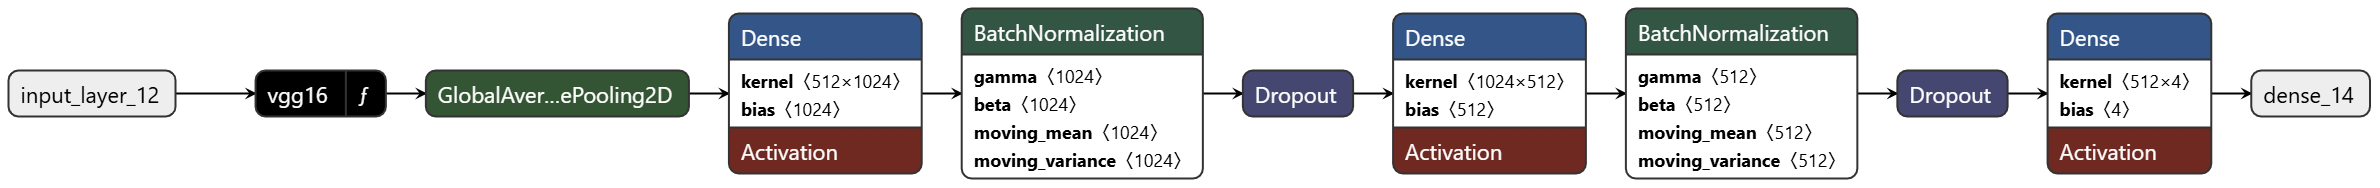
\includegraphics[width=1.0\linewidth]{model_vgg16_fullsize3.keras (1).png}
    \caption{Model for fourth trial using VGG 16 (unfreeze 8 layers)}
    \label{fig:vgg16result3.png}
\end{figure}

Together, these modifications allow the model to retain the robust feature extraction of VGG16, while also becoming increasingly specialized to our dataset. By expanding the trainable layer depth and enhancing training stability, we aim for higher class-wise recall and F1-scores, especially for harder-to-classify conditions like Viral Pneumonia and COVID-19.

This model achieved significantly improved classification performance with an overall accuracy of 91\% on the test set. All four classes showed high precision and recall values, with particularly strong results for the Normal (F1-score: 0.93) and Viral Pneumonia (F1-score: 0.91) classes. Notably, COVID detection saw a substantial boost in precision (0.99), with a good recall of 0.82, indicating the model is highly confident when predicting COVID-positive cases while still capturing the majority of them. Lung Opacity, often a more ambiguous class, was handled well with an F1-score of 0.89. The macro-averaged F1-score of 0.90 and macro recall of 0.88 reflect balanced performance across classes, even in the presence of class imbalance. These results highlight the success of deeper fine-tuning, batch normalization, and effective learning rate scheduling in adapting the VGG16 model to complex medical image classification tasks (figure:\ref{fig:vgg16result4.png}).

\begin{figure}[h!] % the [h!] helps force it "here"
    \centering
    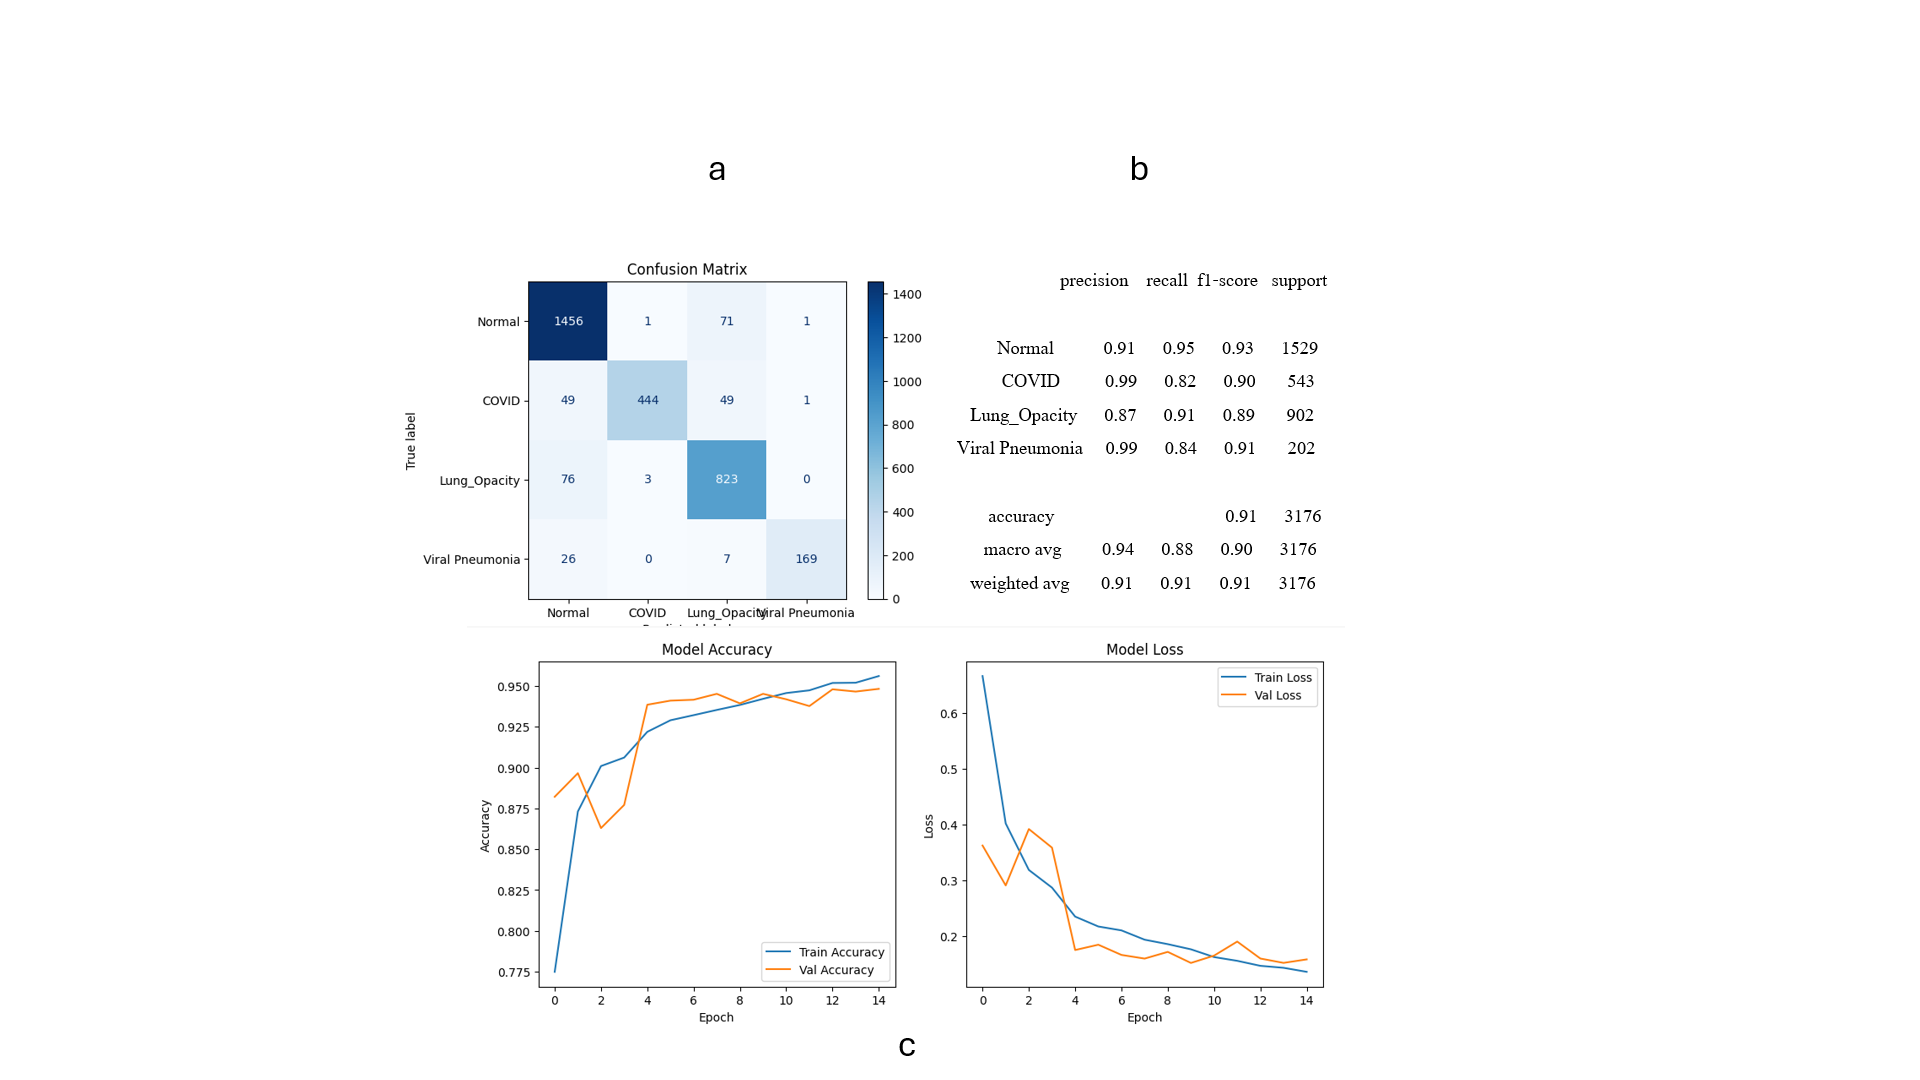
\includegraphics[width=1.0\linewidth]{vgg16-8.png}
    \caption{Results for fourth trial using VGG 16 (unfreeze 8 layers)}
    \label{fig:vgg16result4.png}
\end{figure}
\paragraph{Fifth Trial: Fine-tuning VGG16 Transfer Model: Unfreeze last 15 layers}\mbox{}\\
In this final modification (figure:\ref{fig:vgg16result5.png}), the model was further refined by unfreezing the last 15 convolutional layers of the VGG16 backbone, allowing for deeper fine-tuning and greater adaptability to the specific patterns present in chest X-ray images. This marks a significant shift from earlier stages, where only a few top layers were trainable, as it enables the model to move beyond generic ImageNet features and learn more domain-specific representations. The classification head remained consistent, comprising global average pooling followed by two dense layers with dropout for regularization, culminating in a softmax layer that outputs predictions for the four target classes. To ensure stable and controlled updates during fine-tuning, the model was compiled with a low learning rate of 1e-5 using the Adam optimizer. Additionally, callbacks such as early stopping and learning rate reduction were used to prevent overfitting and encourage efficient convergence. The model checkpoint callback was configured to monitor validation accuracy instead of loss, ensuring that the version of the model with the best classification performance was preserved. These enhancements collectively aimed to boost the model's ability to generalize and perform reliably across all classes, particularly the challenging ones like COVID-19 and Viral Pneumonia.
\begin{figure}[h!] % the [h!] helps force it "here"
    \centering
    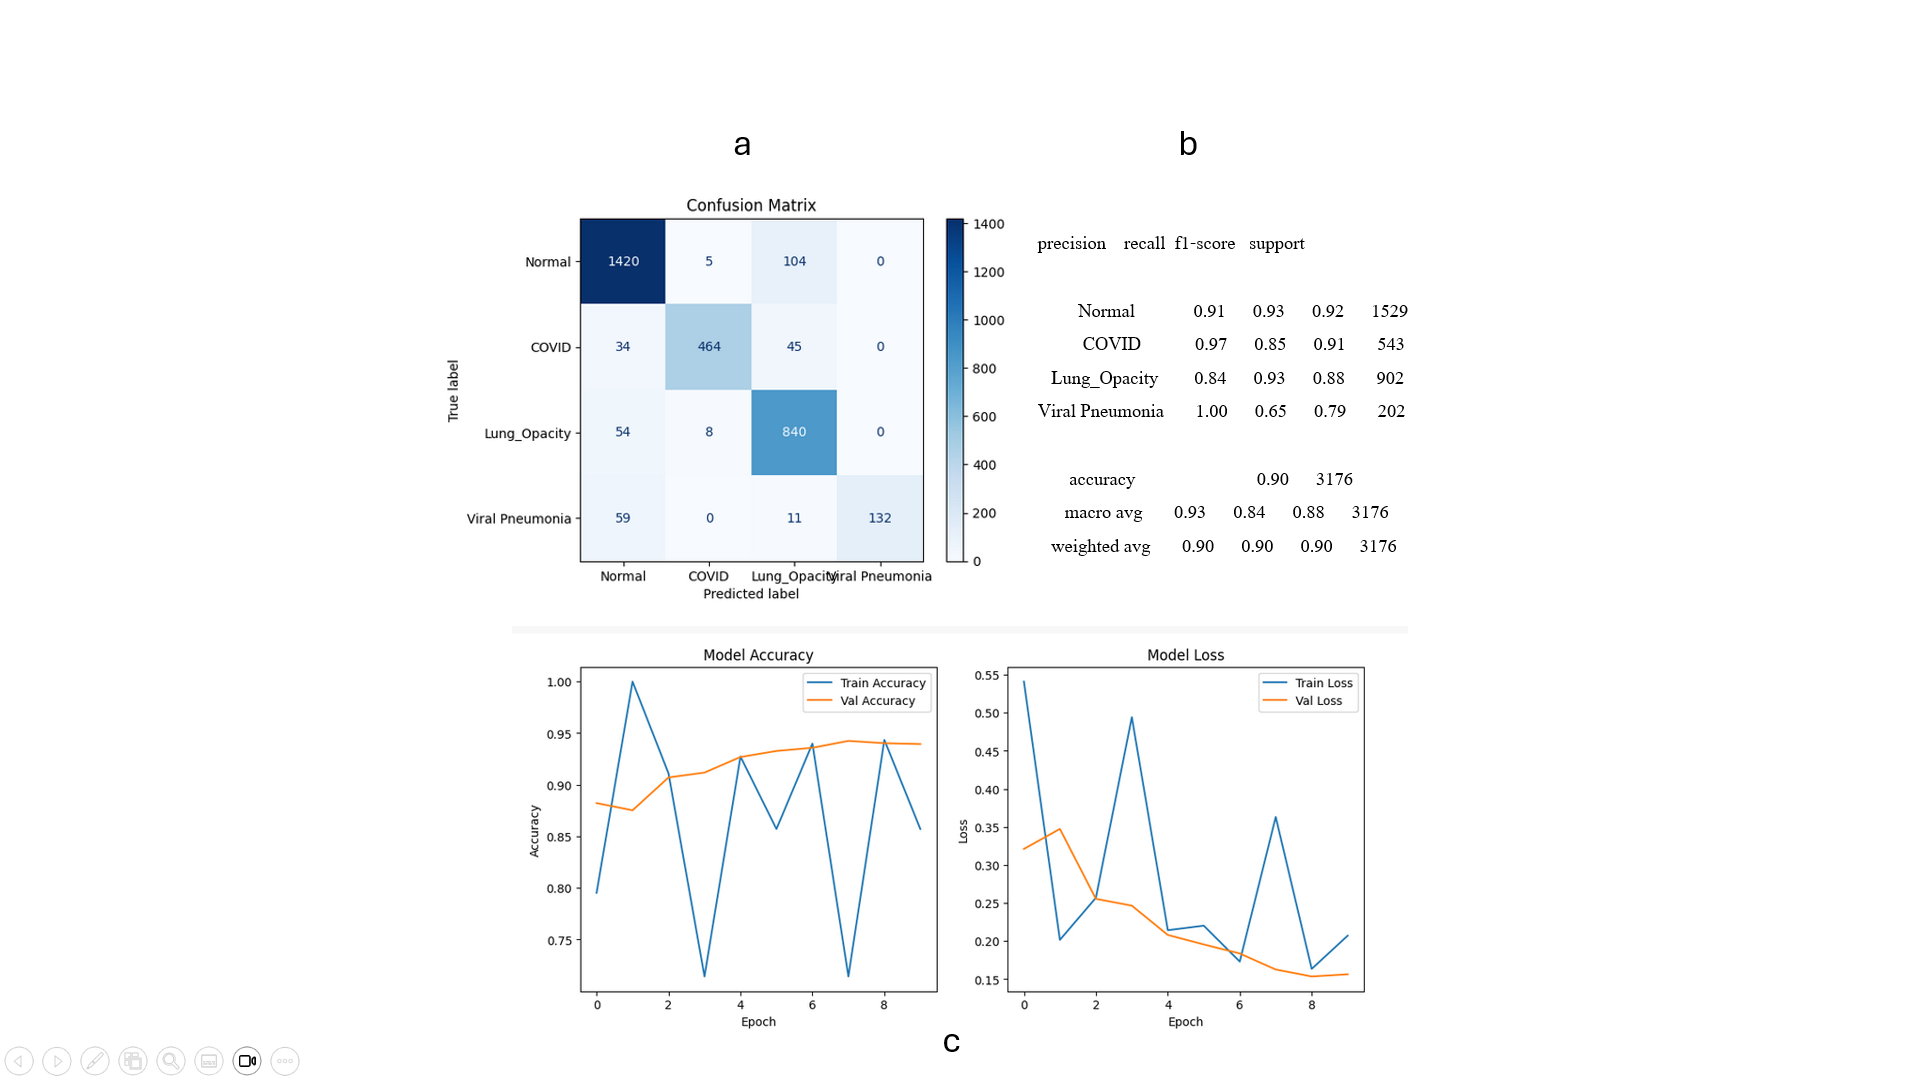
\includegraphics[width=1.0\linewidth]{vgg15-15.png}
    \caption{Results for fourth trial using VGG 16 (unfreeze 15 layers)}
    \label{fig:vgg16result5.png}
\end{figure}
The results from the final model, where the last 15 layers of VGG16 were unfrozen for fine-tuning, show a strong overall performance with an accuracy of 90\% and a weighted F1-score of 0.90 across the four classes. Precision remained high for all classes, particularly for Viral Pneumonia, which achieved perfect precision (1.00), though its recall dropped significantly to 0.65, indicating many false negatives. Normal and Lung\_Opacity classes were predicted with high consistency, achieving F1-scores of 0.92 and 0.88 respectively. 
However, compared to the previous model where only the last 8 layers were unfrozen, this result did not show a clear improvement. In fact, the 8-layer fine-tuned model had higher recall and F1-scores for most classes, suggesting better generalization and balance across the dataset. The drop in recall for *Viral Pneumonia* in this attempt, despite the higher model flexibility, points to possible overfitting or instability due to too many trainable parameters. This outcome highlights that more aggressive fine-tuning does not always guarantee better performance and that a well-calibrated balance between fixed and trainable layers often yields the most robust results.

\paragraph{Sixth Trial: Fine-tuning VGG16 Transfer Model:SE block}\mbox{}\\
This code introduces an advanced variation of the VGG16-based classification model by incorporating a **Squeeze-and-Excitation (SE) block**, a well-known attention mechanism designed to enhance feature representations. The SE block is applied after the last convolutional layer of the VGG16 model (`block5\_conv3`). Its role is to recalibrate the channel-wise feature responses by learning per-channel weights, thus emphasizing informative features while suppressing less useful ones. This refinement helps the model focus on critical parts of the image, which is particularly valuable in medical image analysis like chest X-rays.

After inserting the SE block, the model continues with a classification head composed of global average pooling, two fully connected (Dense) layers with dropout regularization, and a final softmax layer to predict one of the four target classes. The model is partially fine-tuned by unfreezing the last 15 layers, allowing deeper adaptation to the target domain while retaining most of the pretrained weights from ImageNet to avoid overfitting.

Finally, the model is compiled using the Adam optimizer with a low learning rate (`1e-5`), suitable for fine-tuning, and is set up to use sparse categorical crossentropy since class labels are assumed to be integer-encoded. This setup aims to boost performance through better feature utilization while balancing generalization and specificity.

\begin{figure}[h!] % the [h!] helps force it "here"
    \centering
    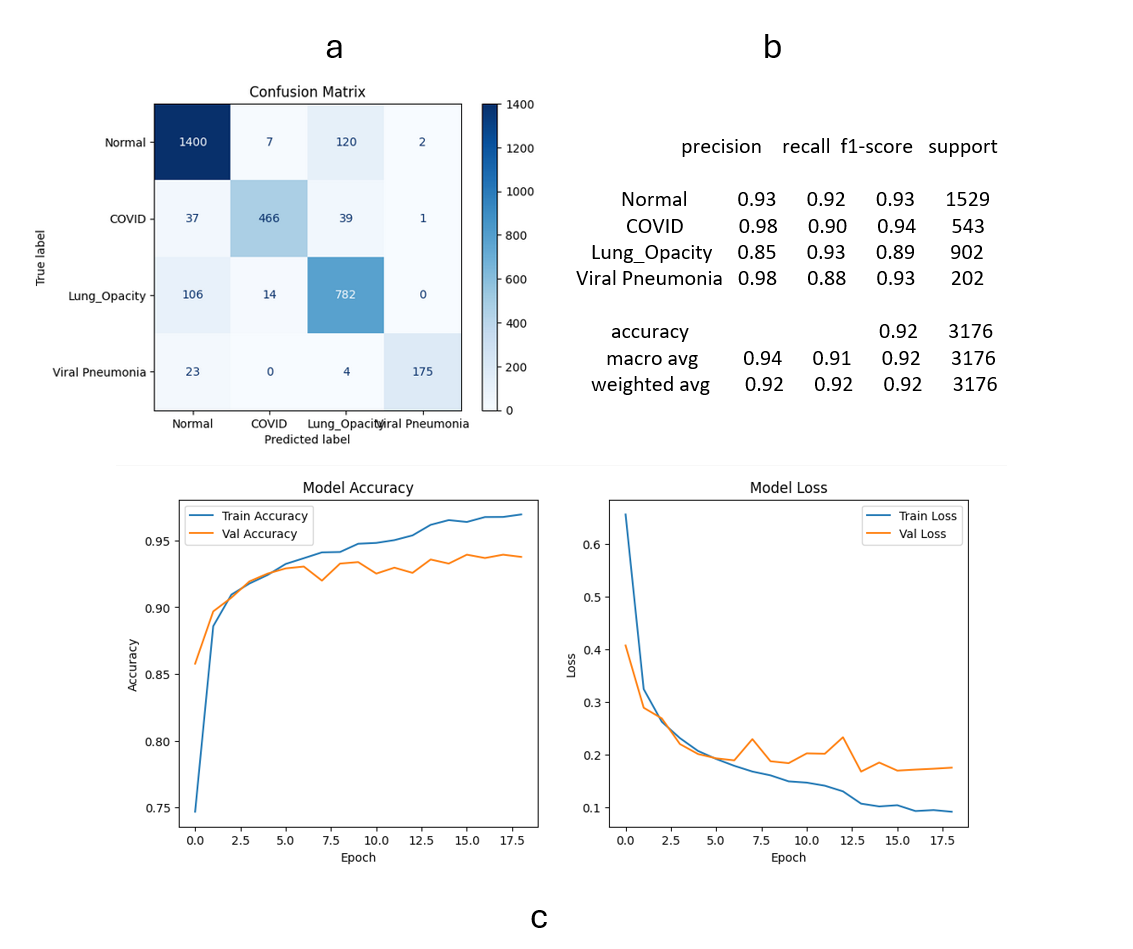
\includegraphics[width=1.0\linewidth]{vgg16se.png}
    \caption{Results for fourth trial using VGG 16 + SE block}
    \label{fig:vgg16result+se.png}
\end{figure}

The performance metrics in this latest result (figure:\ref{fig:vgg16result+se.png}) indicate that incorporating the Squeeze-and-Excitation (SE) block and fine-tuning the last 15 layers of VGG16 produced only marginal improvements over the previous best configuration, which had unfreezing of 8 layers. The overall accuracy stands at 92\%, with strong precision, recall, and F1-scores across all four classes, particularly for Normal, COVID, and Viral Pneumonia.

However, these gains are not significantly higher than those achieved with fewer trainable layers and without the SE block. For example, the F1-score for Lung\_Opacity remained similar (~0.89), and COVID detection performance was already strong in earlier trials. The model’s macro average F1-score increased slightly to 0.92, indicating a consistent performance across classes, but not a dramatic change.

This suggests that while adding attention mechanisms like SE blocks and unfreezing more layers may enhance the model’s feature learning capacity, the benefit plateaus beyond a certain point, especially when earlier configurations were already well-optimized. In essence, the model’s performance has stabilized, and further architectural complexity or layer unfreezing yields diminishing returns in terms of classification accuracy.

\subsubsection{EfficientNet}
The performance of the EfficientNet model on the multi-class classification task revealed varied effectiveness across different categories. The model achieved the highest precision and recall for the Normal class, with a precision of 0.61 and recall of 0.88, resulting in a solid F1-score of 0.72, indicating reliable identification of normal cases. However, the COVID class suffered from poor recall (0.07) and low precision (0.28), yielding a very weak F1-score of 0.11, which suggested significant difficulty in correctly detecting COVID cases. Similarly, Lung Opacity showed moderate performance with balanced precision and recall around 0.54 and 0.50 respectively, leading to an F1-score of 0.52. The Viral Pneumonia class performed the worst, with zero precision, recall, and F1-score, indicating that the model failed to correctly identify any instances of this category. Overall, the model attained an accuracy of 58\%, but the macro average metrics are low (precision, recall, and F1-score all around 0.34), reflecting poor generalization across all classes. Given the low recall and F1-scores for these critical classes, we decided not to move forward with this model and instead explored other approaches to improve classification performance.

\subsubsection{InceptionV3}
\paragraph{Data pre-processing for InceptionV3 model}\mbox{}\\
In order to make it easier to make changes in the input data, we decided that the processing of the input data should not be done offline before the modelling, but instead doing on the fly before starting to train the model. 
The data has been split into train data (85\%) and test data (15\%). Then the train data has been re-split into the final train data (80\%) and validation data (20\%) which is used for validation during training the model. 
The next step was to get rid of the imbalance between the 4 classes. We needed a lot of training runs to figure out which pre-processing should be done in order to use the data for an InceptionV3 model. During these tests all layers of the pretrained model had been frozen. 
These tests showed that we needed to use a dataset for training where the class imbalanced had been fixed by data augmentation. To augment only the minority classes (COVID, Lung Opacity and Viral Pneumonia) and use only the original images for the Normal-class did not work. This has led to the Normal-class was not predicted at all. The confusion matrices of these test all looked something like this, c. f. figure \ref{fig:vgg16_yb_03_cm_norm.png}.
\begin{figure}%[h!] % the [h!] helps force it "here"
    \centering
    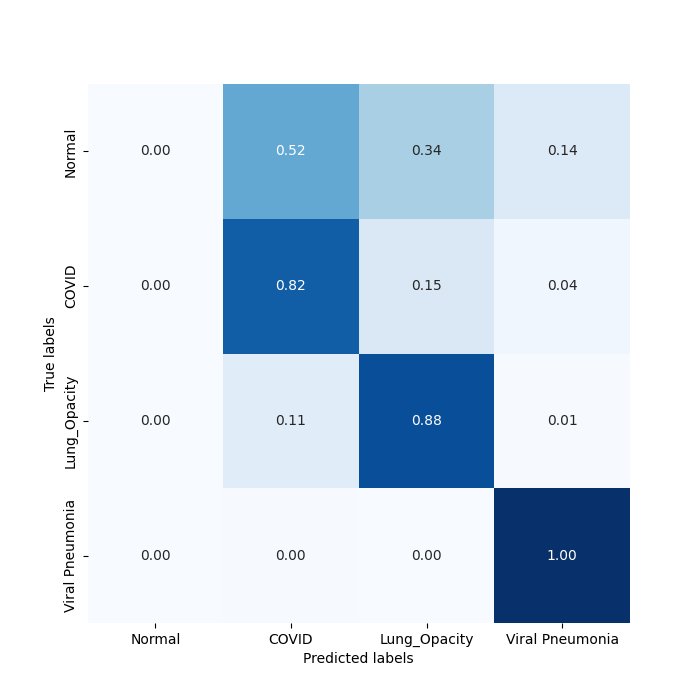
\includegraphics[width=0.5\linewidth]{vgg16_yb_03_cm_norm.png}
    \caption{Example of representative confusion matrix of the input data pre-processing tests.}
    \label{fig:vgg16_yb_03_cm_norm.png}
\end{figure}
The confusion matrices showed that the Normal-class could not be predicted at all and the Viral Pneumonia-class was predicted quite well. This lead to the conclusion, that there must be a difference in the pre-processing of these two classes. For the Normal-class, which is the majority class, only the original, non-augmented images had been used. Whereas for the Viral Pneumonia-class, which is the class containing the least original images, a big number of augmented images had been used for training. 
As a conclusion of these tests we also augmented the Normal-class, by using the original images plus one time augmented images which resulted in 13860 images for the Normal-class in the training dataset. For the training dataset the following number of images had been used: 
\begin{itemize}
\item 'Normal':  13860
\item 'COVID':  14748
\item 'Lung Opacity': 12264 
\item 'Viral Pneumonia':  13725
\end{itemize}
As augmentation technique rotation (of maximum 15°) and translation (of maximum 10\%) had been used. 
No augmentation has been done to the test and validation dataset. 
Before starting the training a random data augmentation was applied to the training data.
\begin{itemize}
\item HorizontalFlip(p=0.5)
\item Rotate(limit=15, p=0.5)
\item ShiftScaleRotate(shift\_limit=0.05, scale\_limit=0.05, rotate\_limit=0, p=0.5) 
\end{itemize}

As a last step the pre-processing function of the pretrained InceptionV3-model (inception\_v3.preprocess\_input) has been applied to train, test and validation set. This returns a preprocessed array with type float32. The input pixel values are scaled between -1 and 1, sample-wise. 

During the different training runs different batch sizes have been tried out (16 and 64). 

\paragraph{The InceptionV3 model}\mbox{}\\
In some papers which handle similar tasks the InceptionV3 model was used. (e.g. "Can AI Help in Screening Viral and COVID-19 Pneumonia?" from Muhammad E. H. Chowdhury et al.). In several sources on the internet it is mentioned that the InceptionV3 model "ensures a balance between performance and computational cost." This is why we thought it could be worth to try using this model on our data. 

The Keras InceptionV3 is a pretrained convolutional neural network that has 311 layers. It has been already trained on more than a million images from the ImageNet database. This pretrained network can classify images into 1000 object categories, such as keyboard, mouse, pencil, and many animals. As a result, the network has learned rich feature representations for a wide range of images. The network has an image input size of 299-by-299. 

\paragraph{1st trial with InceptionV3}\mbox{}\\
For this 1st trial the following settings were used: 
\begin{itemize}
\item input data as described above
\item batch size = 16
\item 10 epochs 
\item Adam optimizer (with default learning rate of 0.001)
\item no callbacks used
\item no fine-tuning has been done
\end{itemize}

The design of the used model is shown in figure \ref{fig:inceptionv3_04.keras_model_design}.
\begin{figure}[ht] % the [h!] helps force it "here"
    \centering
    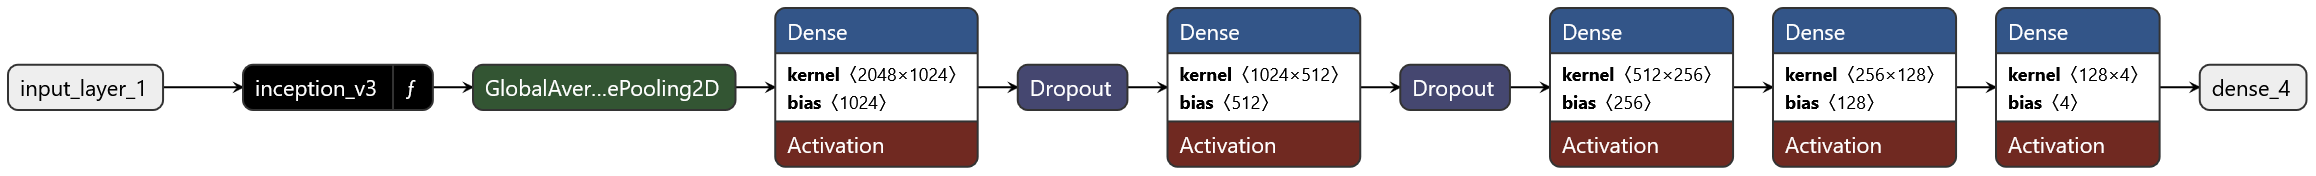
\includegraphics[width=1.0\linewidth]{inceptionv3_04.keras_model_design_nice.png}
    \caption{Model design of 1st trial with InceptionV3}
    \label{fig:inceptionv3_04.keras_model_design}
\end{figure}

The loss and accuracy per epoch in figure \ref{fig:inceptionv3_04_loss_accuracy} show that this model has no good convergence. The classification report and the confusion matrix in figure \ref{fig:inceptionv3_04_results} show that the overall accuracy is only 83\% and that the COVID-class is not very well predicted. The confusion matrix additionally shows that the data augmentation of the Normal-class helped that the Normal-class was predicted better, than as in previous tests (c.f. figure \ref{fig:vgg16_yb_03_cm_norm.png}).

\begin{figure}[ht] % the [h!] helps force it "here"
    \centering
    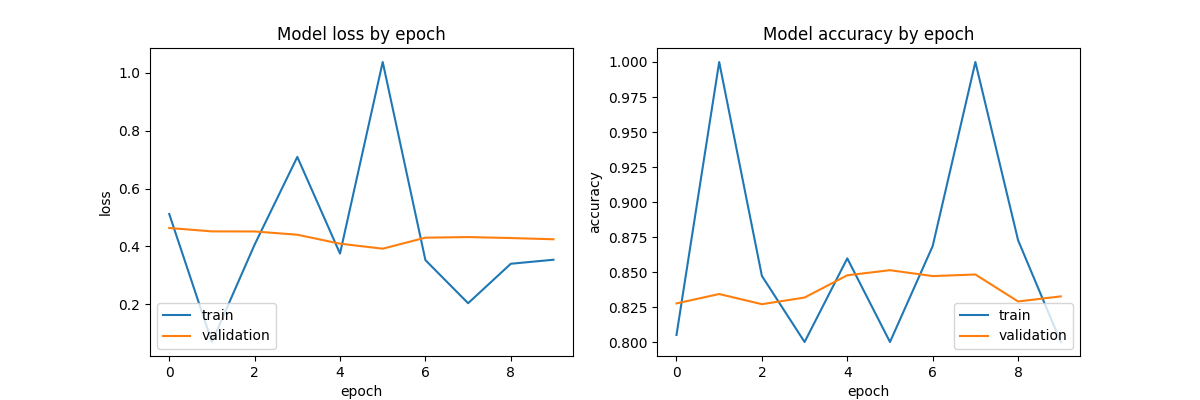
\includegraphics[width=1.0\linewidth]{inceptionv3_04_loss_accuracy.png}
    \caption{Loss and accuracy per epoch of 1st trial with InceptionV3}
    \label{fig:inceptionv3_04_loss_accuracy}
\end{figure}

\begin{figure}[ht]
  \centering
  \subfloat[][]{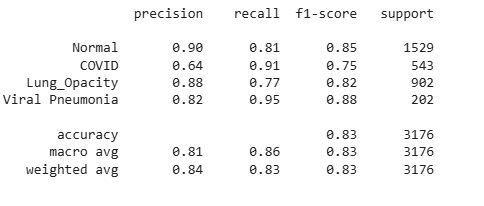
\includegraphics[width=0.4\linewidth]{inceptionv3_04_class_report.png}}%
  \qquad
  \subfloat[][]{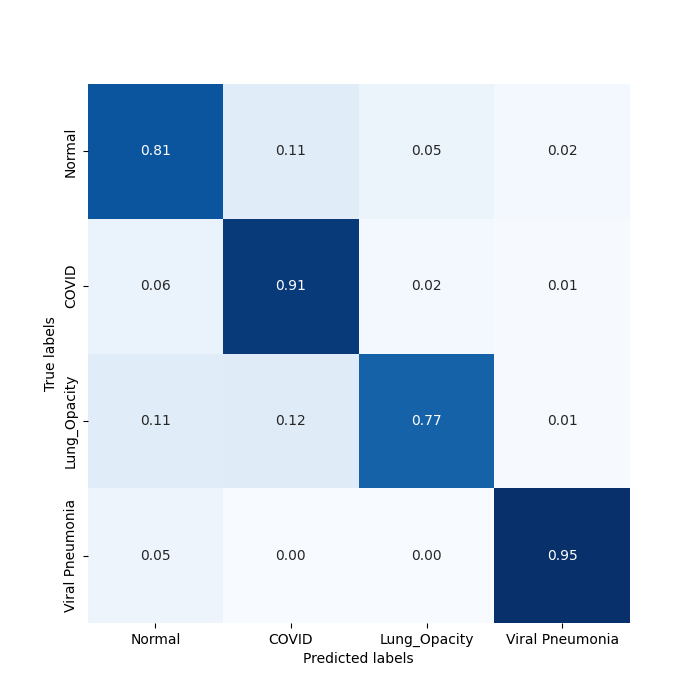
\includegraphics[width=0.4\linewidth]{inceptionv3_04_cm_norm.png}}%
  \caption{classification report and normalized confusion matrix of 1st trial with InceptionV3}
  \label{fig:inceptionv3_04_results}
\end{figure}



\paragraph{2nd trial with InceptionV3}\mbox{}\\
For this 2nd trial the same settings were used than in the 1st trial, but this time callbacks have been used. As the model did not converge within 10 epochs we tried to double the number of epochs for this trial. In summary the following settings were used: 
\begin{itemize}
\item input data as described above
\item batch size = 16
\item 20 epochs 
\item Adam optimizer (with default learning rate of 0.001)
\item callbacks were used (EarlyStopping, Reduce the learning rate and ModelCheckpoint to save the best model)
\item no fine-tuning has been done
\end{itemize}

The design of the used model is shown in figure \ref{fig:inceptionv3_05.keras_model_design}.
\begin{figure}[htb] % the [h!] helps force it "here"
    \centering
    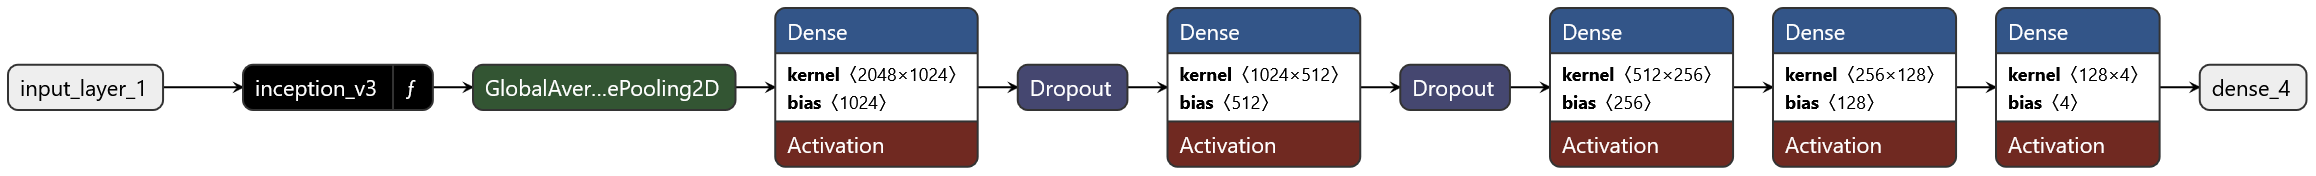
\includegraphics[width=1.0\linewidth]{inceptionv3_05.keras_model_design_nice.png}
    \caption{Model design of 2nd trial with InceptionV3}
    \label{fig:inceptionv3_05.keras_model_design}
\end{figure}

With using the callbacks the learning rate was automatically reduced during training to 1e-05, but the train-loss and train-accuracy per epoch in figure \ref{fig:inceptionv3_05_loss_accuracy} still show a lot of oscillation and therefore no good convergence. The early stopping callback stopped the model after epoch 16 and the best model was the model after epoch 11.\\
The classification report and the confusion matrix in figure \ref{fig:inceptionv3_05_results} show that the overall accuracy is still only 85\% and that the COVID-class is not very well predicted. But compared to the 1st trial the f1-score for the COVID-class increased from 0.75 to 0.81.

\begin{figure}[htb] % the [h!] helps force it "here"
    \centering
    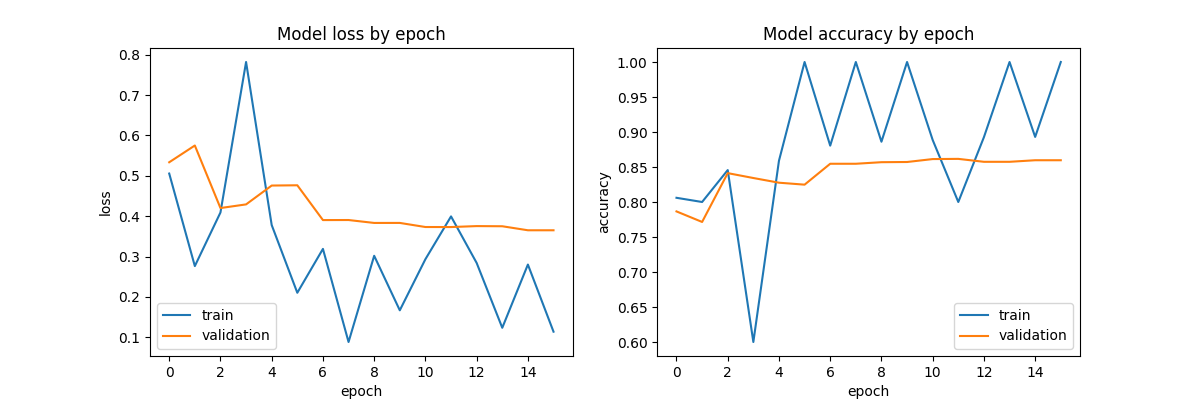
\includegraphics[width=1.0\linewidth]{inceptionv3_05_loss_accuracy.png}
    \caption{Loss and accuracy per epoch of 2nd trial with InceptionV3}
    \label{fig:inceptionv3_05_loss_accuracy}
\end{figure}

\begin{figure}[!h]
  \centering
  \subfloat[][]{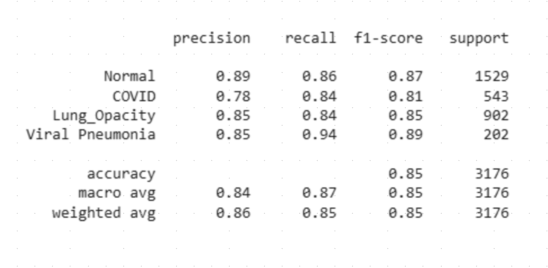
\includegraphics[width=0.4\linewidth]{inceptionv3_05_class_report.png}}%
  \qquad
  \subfloat[][]{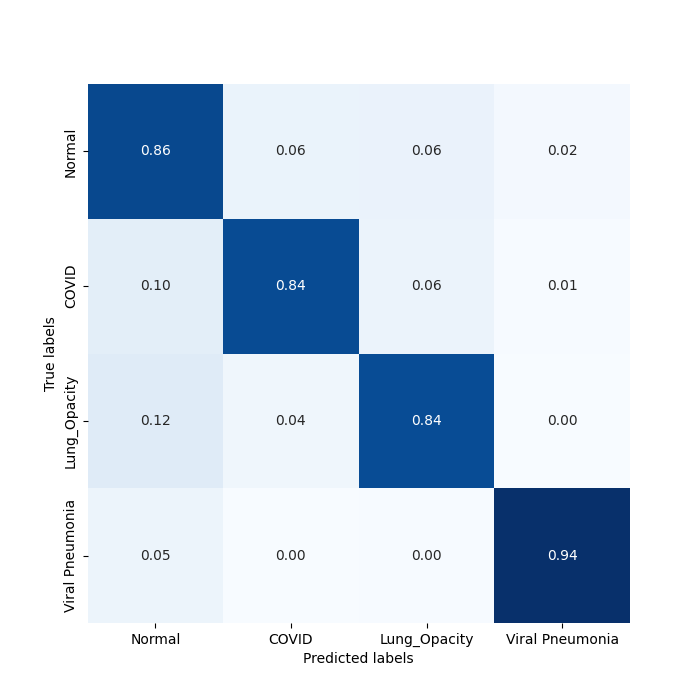
\includegraphics[width=0.4\linewidth]{inceptionv3_05_cm_norm.png}}%
  \caption{classification report and normalized confusion matrix of 2nd trial with InceptionV3}
  \label{fig:inceptionv3_05_results}
\end{figure}

\paragraph{3rd trial with InceptionV3}\mbox{}\\
For this 3rd trial the same settings were used than in the 2nd trial, but this time the batch size was increased from 16 to 64. In summary the following settings were used: 
\begin{itemize}
\item input data as described above
\item batch size = 64
\item 20 epochs 
\item Adam optimizer (with default learning rate of 0.001)
\item callbacks were used (EarlyStopping, Reduce the learning rate and ModelCheckpoint to save the best model)
\item no fine-tuning has been done
\end{itemize}

The design of the used model is shown in figure \ref{fig:inceptionv3_06.keras_model_design}.
\begin{figure}[ht] % the [h!] helps force it "here"
    \centering
    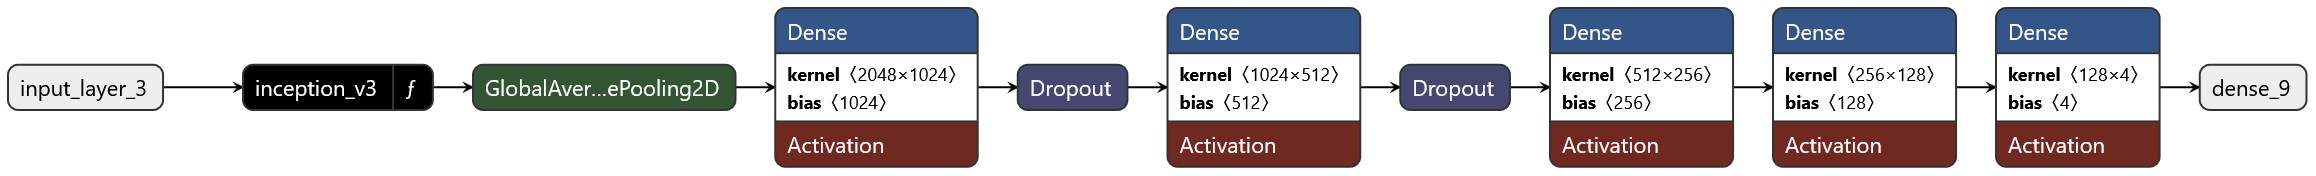
\includegraphics[width=1.0\linewidth]{inceptionv3_06.keras_model_design_nice.png}
    \caption{Model design of 3rd trial with InceptionV3}
    \label{fig:inceptionv3_06.keras_model_design}
\end{figure}

The learning rate was automatically reduced to 1e-05 due to the callback as in the previous test. The best model was saved after 15 epochs. \\
Figure \ref{fig:inceptionv3_06_loss_accuracy} shows that increasing the batch size from 16 to 64 did not fix the oscillation of the train-loss and train-accuracy. And the validation-loss and validation-accuracy stagnates. 

The classification report and the confusion matrix in figure \ref{fig:inceptionv3_06_results} show that the overall accuracy is 86\%  (which is 1\% more than in the 2nd trial). The COVID-class is still the worst predicted class. But at least the f1-score increased by 1\% in this trial compared to the previous trial. 

\begin{figure}[ht] % the [h!] helps force it "here"
    \centering
    \includegraphics[width=1.0\linewidth]{inceptionv3_06_loss_accuracy.png}
    \caption{Loss and accuracy per epoch of 3rd trial with InceptionV3}
    \label{fig:inceptionv3_06_loss_accuracy}
\end{figure}

\begin{figure}[!ht]
  \centering
  \subfloat[][]{\includegraphics[width=0.4\linewidth]{inceptionv3_06_class_report.png}}%
  \qquad
  \subfloat[][]{\includegraphics[width=0.4\linewidth]{inceptionv3_06_cm_norm.png}}%
  \caption{classification report and normalized confusion matrix of 3rd trial with InceptionV3}
  \label{fig:inceptionv3_06_results}
\end{figure}


\paragraph{4th trial with InceptionV3}\mbox{}\\

For this 4th trial the same settings were used than in the 3rd trial, but this time the last 4 layers of the pretrained InceptionV3 model were unfrozen. Additionally, the learning rate was reduced to 1e-05. Some of the parameters of the used callbacks were changed. In summary the following settings were used: 
\begin{itemize}
\item input data as described above
\item batch size = 64
\item 20 epochs 
\item Adam optimizer (with learning rate of 1e-05)
\item callbacks were used (EarlyStopping, Reduce the learning rate and ModelCheckpoint to save the best model)
\item first try of fine-tuning by unfreeze the last 4 layers of the InceptionV3 model
\end{itemize}

The design of the used model is shown in figure \ref{fig:inceptionv3_07.keras_model_design}.
\begin{figure}%[ht] % the [h!] helps force it "here"
    \centering
    \includegraphics[width=1.0\linewidth]{inceptionv3_07.keras_model_design_nice.png}
    \caption{Model design of 4th trial with InceptionV3}
    \label{fig:inceptionv3_07.keras_model_design}
\end{figure}

The learning rate was automatically reduced to 1e-06 due to the callback. The EarlyStopping callback did not stop the model before 20 epochs. \\
Figure \ref{fig:inceptionv3_07_loss_accuracy} shows that in this test the train-loss and train-accuracy is still oscillating. But a slight improvement over the previous tests can be seen: As the epochs increase, the oscillation of the train-accuracy appears to weaken and the amplitude decreases. Furthermore, the curve of the validation-loss and validation-accuracy behaves a little bit more as expected, compared to previous test. The validation-loss slightly decreases with epoch and the validation-accuracy slightly increases with epoch. 

Although the stability of the model looks slightly better, the classification report and the confusion matrix in figure \ref{fig:inceptionv3_07_results} show that the overall accuracy reduced by 3\% compared to the previous test. The COVID-class is still the worst predicted class. \\ 

\begin{figure}%[htb] % the [h!] helps force it "here"
    \centering
    \includegraphics[width=1.0\linewidth]{inceptionv3_07_loss_accuracy.png}
    \caption{Loss and accuracy per epoch of 4th trial with InceptionV3}
    \label{fig:inceptionv3_07_loss_accuracy}
\end{figure}

\begin{figure}%[!ht]
  \centering
  \subfloat[][]{\includegraphics[width=0.4\linewidth]{inceptionv3_07_class_report.png}}%
  \qquad
  \subfloat[][]{\includegraphics[width=0.4\linewidth]{inceptionv3_07_cm_norm.png}}%
  \caption{classification report and normalized confusion matrix of 4th trial with InceptionV3}
  \label{fig:inceptionv3_07_results}
\end{figure}

\paragraph{5th trial with InceptionV3}\mbox{}\\

For this 5th trial the same settings were used than in the 4th trial, but this time another optimizer has been used: RMSprop instead of Adam. The learning rate 1e-05 was not changed. 
In summary the following settings were used: 
\begin{itemize}
\item input data as described above
\item batch size = 64
\item 20 epochs 
\item RMSprop (with learning rate of 1e-05)
\item callbacks were used (EarlyStopping, Reduce the learning rate and ModelCheckpoint to save the best model)
\item first try of fine-tuning by unfreeze the last 4 layers of the InceptionV3 model
\end{itemize}

The design of the used model is shown in figure \ref{fig:inceptionv3_08.keras_model_design}.
\begin{figure}%[ht] % the [h!] helps force it "here"
    \centering
    \includegraphics[width=1.0\linewidth]{inceptionv3_08.keras_model_design_nice.png}
    \caption{Model design of 5th trial with InceptionV3}
    \label{fig:inceptionv3_08.keras_model_design}
\end{figure}

The learning rate was automatically reduced to 1e-06 due to the callback. The EarlyStopping callback did not stop the model before 20 epochs.\\
Figure \ref{fig:inceptionv3_08_loss_accuracy} shows that in this test using another optimizer caused stronger oscillation in the train-loss and train-accuracy. The classification report and the confusion matrix in figure \ref{fig:inceptionv3_08_results} show that the switch to the RMSprop optimizer was not a good choice. Although the overall accuracy with 83\% is the same as in the previous test (4th trial), the f1-score of the COVID-class decreased.\\ 

\begin{figure}%[htb] % the [h!] helps force it "here"
    \centering
    \includegraphics[width=1.0\linewidth]{inceptionv3_08_loss_accuracy.png}
    \caption{Loss and accuracy per epoch of 5th trial with InceptionV3}
    \label{fig:inceptionv3_08_loss_accuracy}
\end{figure}

\begin{figure}%[!ht]
  \centering
  \subfloat[][]{\includegraphics[width=0.4\linewidth]{inceptionv3_08_class_report.png}}%
  \qquad
  \subfloat[][]{\includegraphics[width=0.4\linewidth]{inceptionv3_08_cm_norm.png}}%
  \caption{classification report and normalized confusion matrix of 5th trial with InceptionV3}
  \label{fig:inceptionv3_08_results}
\end{figure}

\paragraph{6th trial with InceptionV3}\mbox{}\\

For this 6th trial we used again the Adam optimizer and we kept all layers of the InceptionV3 model frozen. For this test we tried to leave out the randomly applied augmentation to all classes. The augmentation to handle the class imbalance in the training data was still used. In summary the following settings were used: 
\begin{itemize}
\item input data as described above
\item batch size = 64
\item 20 epochs 
\item Adam (with learning rate of 1e-05)
\item callbacks were used (EarlyStopping, Reduce the learning rate and ModelCheckpoint to save the best model)
\item no fine-tuning has been done
\item no random augmentation to all classes 
\end{itemize}

The design of the used model is shown in figure \ref{fig:inceptionv3_09.keras_model_design}.
\begin{figure}%[ht] % the [h!] helps force it "here"
    \centering
    \includegraphics[width=1.0\linewidth]{inceptionv3_09.keras_model_design_nice.png}
    \caption{Model design of 6th trial with InceptionV3}
    \label{fig:inceptionv3_09.keras_model_design}
\end{figure}

During the 20 epochs the callback did not automatically reduce the learning rate. The EarlyStopping callback did not stop the model before 20 epochs.\\

Figure \ref{fig:inceptionv3_09_loss_accuracy} shows less oscillation in the train-loss and train-accuracy than in the previous test (5th trial). But the train-accuracy and train-loss of the 4th trial (with unfreezing the last 4 layers and applying random augmentation to all classes) looks better. The validation-loss and validation accuracy look similar as in previous test. 

The classification report and the confusion matrix in figure \ref{fig:inceptionv3_09_results} show that the overall accuracy increased a bit compared to 4th and 5th trial (in which we tried to unfreeze the last 4 layers of the base model).\\ 

\begin{figure}%[htb] % the [h!] helps force it "here"
    \centering
    \includegraphics[width=1.0\linewidth]{inceptionv3_09_loss_accuracy.png}
    \caption{Loss and accuracy per epoch of 6th trial with InceptionV3}
    \label{fig:inceptionv3_09_loss_accuracy}
\end{figure}

\begin{figure}%[!ht]
  \centering
  \subfloat[][]{\includegraphics[width=0.4\linewidth]{inceptionv3_09_class_report.png}}%
  \qquad
  \subfloat[][]{\includegraphics[width=0.4\linewidth]{inceptionv3_09_cm_norm.png}}%
  \caption{classification report and normalized confusion matrix of 6th trial with InceptionV3}
  \label{fig:inceptionv3_09_results}
\end{figure}

\paragraph{7th trial with InceptionV3}\mbox{}\\

The InceptionV3 has 311 layers. For this 7th trial we tried to unfreeze a lot more layers of the pretrained base model. As an example from https://keras.io/api/applications/ we chose to retrain the top 2 inception blocks, i.e. we will freeze the first 249 layers and unfreeze the rest. As recommended in that example we used the SGD(learning\_rate=0.0001, momentum=0.9) optimizer to compile the model. In summary the following settings were used: 
\begin{itemize}
\item input data as described above
\item batch size = 64
\item 20 epochs 
\item SGD(learning\_rate=0.0001, momentum=0.9) optimizer
\item callbacks were used (EarlyStopping, Reduce the learning rate and ModelCheckpoint to save the best model)
\item fine-tuning has been done: freeze only the first 249 layers and unfreeze the rest
\item random augmentation to all classes 
\end{itemize}

The design of the used model is shown in figure \ref{fig:inceptionv3_10.keras_model_design}.
\begin{figure}%[ht] % the [h!] helps force it "here"
    \centering
    \includegraphics[width=1.0\linewidth]{inceptionv3_10.keras_model_design_nice.png}
    \caption{Model design of 7th trial with InceptionV3}
    \label{fig:inceptionv3_10.keras_model_design}
\end{figure}

During the 20 epochs the callback did not automatically reduce the learning rate. The EarlyStopping callback did not stop the model before 20 epochs.\\

Figure \ref{fig:inceptionv3_10_loss_accuracy} still shows a lot of oscillation in the train-loss and train-accuracy. But the train-accuracy and train-loss is nearly the same over all epochs, only a slight increase (accuracy)/ descrease (loss) can be seen over the epochs. 

However, the classification report and the confusion matrix in figure \ref{fig:inceptionv3_10_results} show the best result we reached with the InceptionV3 model so far. An overall accuracy of 91\% and even the COVID-class is well predicted (precision 92\%, recall 91\% and f1-score 91\%).

\begin{figure}%[htb] % the [h!] helps force it "here"
    \centering
    \includegraphics[width=1.0\linewidth]{inceptionv3_10_loss_accuracy.png}
    \caption{Loss and accuracy per epoch of 7th trial with InceptionV3}
    \label{fig:inceptionv3_10_loss_accuracy}
\end{figure}

\begin{figure}%[!ht]
  \centering
  \subfloat[][]{\includegraphics[width=0.4\linewidth]{inceptionv3_10_class_report.png}}%
  \qquad
  \subfloat[][]{\includegraphics[width=0.4\linewidth]{inceptionv3_10_cm_norm.png}}%
  \caption{classification report and normalized confusion matrix of 7th trial with InceptionV3}
  \label{fig:inceptionv3_10_results}
\end{figure}


\paragraph{8th trial with InceptionV3}\mbox{}\\
As the accuracy of the previous test (7th trial) was quite promising, with the same setup another test has been done. The only change was, that this time the corresponding masks hade been apllied to the X-ray images. 
Three tests were carried out.  These differed in that the masks were applied to different data sets. Masks were applied to:
\begin{enumerate}
\item the train dataset
\item the train and validation dataset
\item the train, validation and test dataset
\end{enumerate}

In summary the following settings were used: 
\begin{itemize}
\item input data as described above
\item batch size = 64
\item 20 epochs 
\item SGD(learning\_rate=0.0001, momentum=0.9) optimizer
\item callbacks were used (EarlyStopping, Reduce the learning rate and ModelCheckpoint to save the best model)
\item fine-tuning has been done: freeze only the first 249 layers and unfreeze the rest
\item random augmentation to all classes 
\item corresponding mask is applied to the X-ray image in the train dataset
\end{itemize}

The design of the used model is the same as in the previous test (7th trial, c.f. figure \ref{fig:inceptionv3_10.keras_model_design}.)

When training the model with only masks attached to the training dataset the accuracy and loss does not converge at all, as figure \ref{fig:inceptionv3_11_loss_accuracy} shows. Therefore, the training has been redone with applied masks to the training and validation dataset. If you look at figure \ref{fig:inceptionv3_12_loss_accuracy}, this test looks very promising: The validation loss decreases and the validation accuracy increases. The oscillation of the training loss and accuracy is less than in other tests with the InceptionV3 model, especially in the later epochs there is less oscillation. 

The classification report and the confusion matrix of the training and prediction with only masks applied to the training dataset (figure \ref{fig:inceptionv3_11_results}) show that this model is useless. The classification report and the confusion matrix of the second test (figure \ref{fig:inceptionv3_12_results}) show that the test where the masks have only been applied to the train and validation dataset is useless too. 
The prediction using X-ray images with applied masks are the best option when using masks, figure \ref{fig:inceptionv3_13_results}. But the overall accuracy is only 84\% and also the COVID class is not very well predicted. This test is comparable to the 7th trial. The only difference is that masks have been added here. If we compare the results of the two predictions of these tests, we can conclude, that the model does better predictions without including the masks. In the 7th trial the overall accuracy was 91\% and even the COVID-class had a f1-score of 91\%, c.f figure \ref{fig:inceptionv3_10_results}.

    
\begin{figure}%[htb] % the [h!] helps force it "here"
    \centering
    \includegraphics[width=1.0\linewidth]{inceptionv3_11_loss_accuracy.png}
    \caption{Loss and accuracy per epoch of 8th trial with InceptionV3. Masks applied to the training dataset.}
    \label{fig:inceptionv3_11_loss_accuracy}
\end{figure}

\begin{figure}%[htb] % the [h!] helps force it "here"
    \centering
    \includegraphics[width=1.0\linewidth]{inceptionv3_12_loss_accuracy.png}
    \caption{Loss and accuracy per epoch of 8th trial with InceptionV3. Masks applied to the training and validation dataset.}
    \label{fig:inceptionv3_12_loss_accuracy}
\end{figure}

\begin{figure}%[!ht]
  \centering
  \subfloat[][]{\includegraphics[width=0.4\linewidth]{inceptionv3_11_class_report.png}}%
  \qquad
  \subfloat[][]{\includegraphics[width=0.4\linewidth]{inceptionv3_11_cm_norm.png}}%
  \caption{Classification report and normalized confusion matrix of 8th trial with InceptionV3. Masks applied to the training dataset.}
  \label{fig:inceptionv3_11_results}
\end{figure}

\begin{figure}%[!ht]
  \centering
  \subfloat[][]{\includegraphics[width=0.4\linewidth]{inceptionv3_12_class_report.png}}%
  \qquad
  \subfloat[][]{\includegraphics[width=0.4\linewidth]{inceptionv3_12_cm_norm.png}}%
  \caption{Classification report and normalized confusion matrix of 8th trial with InceptionV3. Masks applied to the training and validation dataset.}
  \label{fig:inceptionv3_12_results}
\end{figure}

\begin{figure}%[!ht]
  \centering
  \subfloat[][]{\includegraphics[width=0.4\linewidth]{inceptionv3_13_class_report.png}}%
  \qquad
  \subfloat[][]{\includegraphics[width=0.4\linewidth]{inceptionv3_13_cm_norm.png}}%
  \caption{Classification report and normalized confusion matrix of 8th trial with InceptionV3. Masks applied to the training, validation and train dataset.}
  \label{fig:inceptionv3_13_results}
\end{figure}

\subsubsection{DenseNet121}
ToDo: Alex Input your results here

\subsubsection{INTERPRETIBILTY OF BEST DEEP LEARNING MODELS:GRAD-CAM}\mbox{}\\

\begin{itemize}
    \item We performed Gradcam on our self built CNN mentioned in section 3.3.1. We first loaded a set of test images along with their corresponding masks, resizing them to a consistent target size and normalizing the pixel values between 0 and 1. The images and their masks are then combined into a single four-channel input (three RGB channels plus one mask channel), which matched the input shape expected by the trained CNN model. We loaded a previously trained Keras model designed to take these four-channel inputs. To interpret the model’s predictions, we implemented the Grad-CAM (Gradient-weighted Class Activation Mapping) technique: this generates heatmaps that highlight the regions in the input image most influential in the model’s decision for a predicted class. We apply Grad-CAM to multiple test images, visualizing the model’s focus areas by overlaying the heatmaps on the original images, and display these annotated images in a grid to better understand and interpret the model’s behavior on the test set, figure \ref{fig:gradcam_CNN}.
\end{itemize}

\begin{figure}[ht] % the [h!] helps force it "here"
    \centering
    \includegraphics[width=1.0\linewidth]{cnngradcamoutput.png}
    \caption{GRADCAM on CNN}
    \label{fig:gradcam_CNN}
\end{figure}
\begin{itemize}
    \item The second model on which we ran gradcan interpretibilty was our VGG16 transfer learning model with last 8 layers unfrozen. In this project, we implemented Grad-CAM (Gradient-weighted Class Activation Mapping) to visually interpret the decisions made by a deep learning model. First, we loaded and preprocessed a test image using OpenCV, where we resized it to 224x224 pixels, converted it to RGB format, and applied model-specific preprocessing (such as scaling). Then, we loaded our trained model from disk. To generate the Grad-CAM heatmap, we built a modified version of the model that outputs both the activations from a specific convolutional layer and the final prediction. Using TensorFlow's gradient tracking, we computed the gradients of the predicted class score with respect to the chosen convolutional layer's outputs. These gradients were pooled and used to weight the feature maps, resulting in a heatmap that highlights the most important regions in the image. We then overlaid this heatmap onto the original image to create a visual explanation of the model's prediction. Finally, we displayed the original image, the Grad-CAM heatmap, and the overlay side by side using Matplotlib, allowing us to clearly see which parts of the image influenced the model’s decision the most, figure \ref{fig:gradcam_vgg16}.
\end{itemize}
   
\begin{figure}[ht] % the [h!] helps force it "here"
    \centering
    \includegraphics[width=1.0\linewidth]{vgg16gradcam.png}
    \caption{GRADCAM on VGG16 Transfer model}
    \label{fig:gradcam_vgg16}
\end{figure}



\section{Conclusion}
Todo: "Scientific and business conclusions based on the success or failure of the modeling." \\

Which model performed best? Which model do we chose as a conclusion of all our tests? \\
Can that model be used? Is it reliable enough? Do we have optimization proposals? \\

\end{document}